\chapter{直线和平面}
\section{空间图形}
在初中几何课中,我们讨论的几何图形和几何问题,主
要局限在一个平面上.然而,我们生活着的现实世界却是具
有长、宽、高的所谓“三维空间”.而平面只是我们生活空
间的某个断面.我们日常所见的形体,如桌椅、房屋、球、
漏斗等等,它们并不局限在一个平面上,都是立体的.为了
精确地认识这些实际存在的形体,以便为我们的生产和生活
服务,我们必须学习有关空间图形的知识.

我们知道平面图形是同一平面上的点的集合,而\textbf{空间图
形却是不全在同一平面上的点的集合}.例如正方体、三棱
锥、圆柱、球等都是空间图形.空间图形也叫立体图形.我
们将在平面几何知识的基础上,来研究空间图形的性质、画
法以及有关的计算和应用.

\begin{figure}[htp]
    \centering
\begin{tikzpicture}[>=latex, scale=.5]
\begin{scope}
\tkzDefPoints{0/0/A, 3/0/B, -1/1/D, 0/3/A'}
\tkzDefPointsBy[translation= from A to D](B){C}
\tkzDrawSegments(A,B A,D)
\tkzDefPointsBy[translation= from A to A'](B,C,D){B',C',D'}
\tkzDrawPolygon(A',B',C',D')
\tkzDrawSegments(A,B A,D)
\tkzDrawSegments(A,A' B,B' D,D')
\tkzDrawSegments[dashed](C,B C,D C,C')
\node at (1,-1){立方体};

\end{scope}
\begin{scope}[xshift=5cm]
    \tkzDefPoints{-.5/1/A, 3.5/1/B, .8/0/C, 1.5/4/D}
\tkzDrawPolygon(A,C,B,D)
\tkzDrawSegments(C,D)
\tkzDrawSegments[dashed](A,B)
\node at (1.5,-1){三棱锥};
\end{scope}
\begin{scope}[xshift=10cm]
\tkzDefPoints{0/.5/A, 4/.5/B, 4/3.5/C, 0/3.5/D}
\draw(A) arc [start angle =-180, end angle =0, x radius=2, y radius=.5];
\draw[dashed](A) arc [start angle =180, end angle =0, x radius=2, y radius=.5];
\draw(D) arc [start angle =-180, end angle =0, x radius=2, y radius=.5];
\draw(D) arc [start angle =180, end angle =0, x radius=2, y radius=.5];
\node at (2,-1){圆柱};
\tkzDrawSegments(A,D B,C)
\end{scope}

\begin{scope}[xshift=15cm, yshift=2cm]
\tkzDefPoints{2.828/0/A, -2+2.828/0/B}
\tkzDefPoint(45:2){C}
\tkzDefPoint(-45:2){D}
\draw(A) circle (2);
\draw(B) arc [start angle =-180, end angle =0, x radius=2, y radius=.5];
\draw[dashed](B) arc [start angle =180, end angle =0, x radius=2, y radius=.5];
\draw[dashed,rotate=-45](C) arc [start angle =-180, end angle =0, x radius=2, y radius=.5];
\draw[rotate=-45](C) arc [start angle =180, end angle =0, x radius=2, y radius=.5];
\draw[dashed,rotate=45](D)  arc [start angle =-180, end angle =0, x radius=2, y radius=.5];
\draw[rotate=45](D) arc [start angle =180, end angle =0, x radius=2, y radius=.5];
\node at (3,-3){球};
\end{scope}

\end{tikzpicture}   
    \caption{}
\end{figure}

空间图形是在平面上(纸上)画出来的表示立体的图.
如在图1.1中,各图都表示出了某种立体.这种图形叫直
观图.除了用直观图表示立体以外,还有其他表示立体的方
法,如展开图和投影图等等.下面我们作些简要的介绍.

\subsection{直观图}
\subsubsection{水平放置的平面图形的画法}
当我们把一个正方形和圆放置在水平位置观察时,我们
的视觉会产生一些变化,总觉得它们像平行四边形和椭圆.
它们会变成怎样的平行四边形和椭圆呢?由于观察的角度不
同,会有不同的形状,这就涉及到了水平平面图形的画法问
题,下面就是较常用的两种画法.

第一种画法

\begin{example}
    画正方形的直观图.
\end{example}

\begin{figure}[htp]
    \centering
    \begin{tikzpicture}[>=latex,scale=1.5]
     \begin{scope}
\draw[<->](1.5,0)node[right]{$X$}--(0,0)--(0,1.5)node[right]{$Y$};
\draw(0,0)node[below]{$A$}--(1,0)node[below]{$B$}--(1,1)node[right]{$C$}--(0,1)node[left]{$D$};
\node at (.8,-.5,0){$(1)$};
\end{scope}   
\begin{scope}[xshift=3cm, x={(0:1cm)},y={(45:.5cm)},z={(90:1cm)}]
    \draw[<->](2,0,0)node[right]{$X'$}--(0,0,0)--(0,2,0)node[right]{$Y'$};
    \draw(0,0,0)node[below]{$A'$}--(1,0,0)node[below]{$B'$}--(1,1,0)node[right]{$C'$}--(0,1,0)node[left]{$D'$};
    \node at (1.5,-1.414,0){$(2)$};
    \end{scope}      
    \end{tikzpicture}
    \caption{}
\end{figure}

\textbf{画法}
\begin{enumerate}
    \item 在正方形$ABCD$上,分别取$AB$、$AD$为$X$轴
和$Y$轴,它们互相垂直于$A$点.

画对应的$X'$轴和$Y'$轴,使$\angle X'A'Y'=45^{\circ}$.
\item 在$X'$轴上截取$A'B'=AB$, 在$Y'$轴上截取
$A'D'=\frac{1}{2}AD$

\item 以$A'B'$、$A'D'$为邻边画平行四边形
$A'B'C'D'$就是正方形$ABCD$的直观图.(图1.2).
\end{enumerate}

\begin{example}
    画正五边形的直观图.
\end{example}


\begin{figure}[htp]
    \centering
    \begin{tikzpicture}[>=latex,scale=1.2]
     \begin{scope}
\draw[<-](0,4)node[right]{$Y$}--(0,-.5); 
\draw[->](-2,0)--(2,0)node[right]{$X$};
\draw(-1,0)node[below]{$A$}--(1,0)node[below]{$B$}--(1.62,1.9)node[right]{$C$}--(0,3.08)node[right]{$D$}--(-1.62,1.9)node[left]{$E$}--(-1,0);
\draw[dashed](-1.62,1.9)--(-1.62,0)node[below]{$E_1$};
\draw[dashed](1.62,1.9)--(1.62,0)node[below]{$C_1$};
\node at (.25,-.25){$O$};
\node at (0,-1){$(1)$};
\end{scope}   
\begin{scope}[xshift=5cm, x={(0:1cm)},y={(45:.5cm)},z={(90:1cm)}]
    \draw[<-](0,6)node[right]{$Y'$}--(0,-1); 
    \draw[->](-2,0)--(3,0)node[right]{$X'$};
    \draw(-1,0)node[below]{$A'$}--(1,0)node[below]{$B'$}--(1.62,1.9)node[right]{$C'$}--(0,3.08)node[right]{$D'$}--(-1.62,1.9)node[left]{$E'$}--(-1,0);
    \draw[dashed](-1.62,1.9)--(-1.62,0)node[below]{$E'_1$};
    \draw[dashed](1.62,1.9)--(1.62,0)node[below]{$C'_1$};
    \node at (.25,-.5){$O'$};
    \node at (1,-2.828,0){$(2)$};
    \end{scope}      
    \end{tikzpicture}
    \caption{}
\end{figure}

\textbf{画法}
\begin{enumerate}
    \item 取正五边形$ABCDE$的$AB$所在直线为$X$轴,
    取$AB$的中垂线为$Y$轴($Y$轴必过$D$点),两轴交于$O$点.
    (图1.3(1))

    画对应的$X'$轴,$Y'$轴,使$\angle X'O'Y'=45^{\circ}$
    \item 作$CC_1\bot X$轴于$C_1$, 作$EE_1\bot X$轴于$E_1$, 在
    $X'$轴上取$A'B'=AB$, 且使$O'$为$A'B'$中点,并在$X'$轴
    上分别取$C'_1$点和$E'_1$点,使$O'C'_1=OC_1$, $O'E'_1=OE_1$.
    \item 在$Y'$轴上截取$O'D'=\frac{1}{2}OD$, 并引$E'_1E'\parallel
    O'Y'$, 且使$E'_1E=\frac{1}{2}E_1E$, 引$C_1'C'\parallel O'Y'$, 且使
    $C'_1C'=\frac{1}{2}C_1C$.
    \item 连结$A'E'$、$E'D'$、$D'C'$、$C'B'$, 则五边
    形$A'B'C'D'E'$就是正五边形$ABCDE$的直观图.(图
    1.3(2))
\end{enumerate}

通过上面例题,我们可以得出这种画法的规则如下:
\begin{enumerate}
\item 在图形上取互相垂直的$X$轴、$Y$轴,并画出与之
对应的$X'$轴,$Y'$轴,使$\angle X'O'Y'=45^{\circ}$(或$135^{\circ}$), $X'$
轴和$Y'$轴所确定的平面表示水平平面.
\item 图形中平行于$X$轴或$Y$轴的线段(包括在轴上的
线段)分别画成平行于$X'$轴和$Y'$轴的线段.
\item 平行于$X$轴的线段,长度不变;平行于$Y$轴的线
段,长度变为原来的一半.
\end{enumerate}

第二种画法

\begin{example}
   画圆的直观图 

   圆的直观图是一个椭圆,常采用如下近似画法:
\begin{enumerate}
    \item 取$\odot O$的一对互相垂直的直径$AB$, $CD$分别为$X$
轴、$Y$轴,并画出对应的$X'$轴、$Y'$轴,使$\angle X'O'Y'=120^{\circ}$.
\item 在$O'X'$上取$O'A'=OA$, 并取$A'$关于$O'$的对称
点$B'$, 然后在$O'Y'$轴上取$O'C'=OC$, 并取$C'$关于$O'$的对
称点$D'$.
\item 过$A'$、$B'$作$O'Y'$的平行线,过$C'$、$D'$作$O'X'$
的平行线,所作四条直线交出一个菱形,设$E$、$F$是菱形关
于$O'$点对称的顶点.
\item 连$ED'$, $FA'$, 交于$G$; 连$EB'$、$FC'$交于$H$.
\item 以$E$为心,以$ED'$为半径,作$\wideparen{D'B'}$, 以$F$为心,
以$FA'$为半径作$\wideparen{A'C'}$, 以$G$为心,以$GA'$为半径作$\wideparen{D'A}$,
以$H$为心,以$HC'$半径作$\wideparen{B'C'}$, 则此四弧连接成一个近似椭
圆.(图1.4(2))
\end{enumerate}

\begin{figure}[htp]
    \centering
    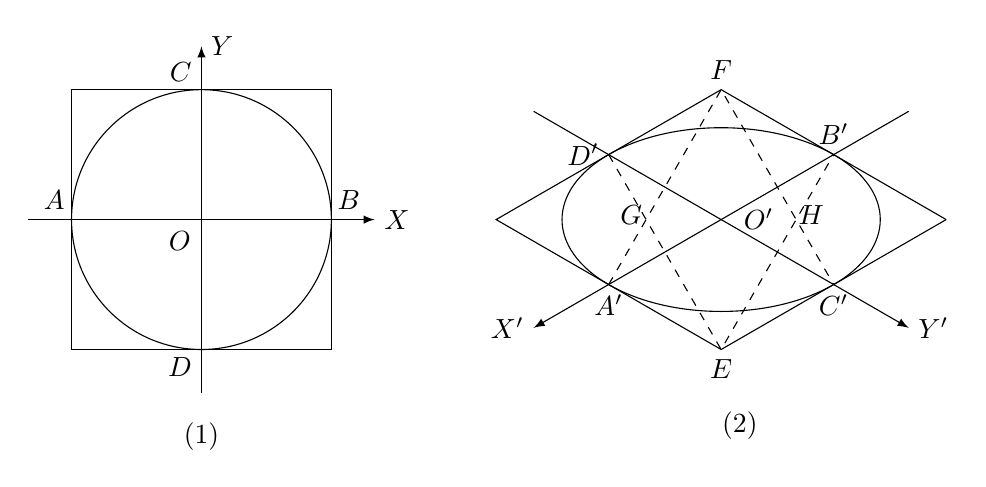
\begin{tikzpicture}[>=latex,scale=1.1]
     \begin{scope}
\draw[<-](0,2)node[right]{$Y$}--(0,-2); 
\draw[->](-2,0)--(2,0)node[right]{$X$};
\draw(-1.5,-1.5)--(-1.5,1.5)--(1.5,1.5)--(1.5,-1.5)--(-1.5,-1.5);
\draw (0,0) circle (1.5);
\node at (-1.7,0)[above]{$A$};
\node at (1.7,0)[above]{$B$};
\node at (0,1.7)[left]{$C$};
\node at (0,-1.7)[left]{$D$};
\node at (-.25,-.25){$O$};
\node at (0,-2.5){$(1)$};
\end{scope}   
\begin{scope}[xshift=6cm, x={(-150:1cm)},y={(150:1cm)}]
    \draw[->](0,2.5)--(0,-2.5)node[right]{$Y'$}; 
    \draw[->](-2.5,0)--(2.5,0)node[left]{$X'$};
    \draw(-1.5,-1.5)--(-1.5,1.5)--(1.5,1.5)--(1.5,-1.5)--(-1.5,-1.5);
    \draw (0,0) circle (1.5);
    \node at (-1.5,0)[above]{$B'$};
    \node  at (1.5,0)[below]{$A'$};
    \node  at (0,1.5) [left]{$D'$};
    \node  at (0,-1.5)[below]{$C'$};
    \node  at (-.25,-.25){$O'$};
    \node  at (.55,.65){$G$};
    \node  at (-.65,-.55){$H$};
    \draw[dashed](0,1.5)--(1.5,-1.5)node[below]{$E$}--(-1.5,0);
    \draw[dashed](1.5,0)--(-1.5,1.5)node[above]{$F$}--(0,-1.5);
    \node at (2.25,-2.5){$(2)$};
    \end{scope}      
    \end{tikzpicture}
    \caption{}
\end{figure}

从上述画法中,我们看出圆的中心$O$, 变成了椭圆的中
心$O'$, 圆的一对互相垂直的直径(如$AB$、$CD$)变成椭圆
的一对直径(如$A'B'$, $C'D'$),它们叫做椭圆的共轭直
径,实际上如果知道了一对椭圆的共轭直径,就可以把椭圆
近似地画出来了.

更省事的办法是用椭圆模板(图1.5)经过椭圆的一对
共轭直径端点来画椭圆.
\begin{figure}[htp]
    \centering
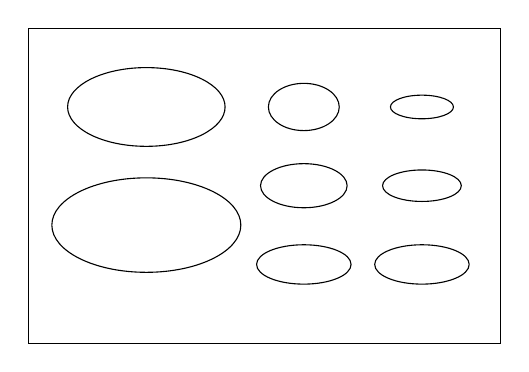
\begin{tikzpicture}[>=latex]
\draw(0,0) rectangle (6,4);
\draw(1.5,1.5) ellipse[x radius=1.2, y radius=.6];
\draw(1.5,3) ellipse[x radius=1, y radius=.5];
\draw(3.5,3) ellipse[x radius=.45, y radius=.3];
\draw(3.5,2) ellipse[x radius=.55, y radius=.28];
\draw(3.5,1) ellipse[x radius=.6, y radius=.25];
\draw(5,3) ellipse[x radius=.4, y radius=.15];
\draw(5,2) ellipse[x radius=.5, y radius=.2];
\draw(5,1) ellipse[x radius=.6, y radius=.25];
\end{tikzpicture}
    \caption{}
\end{figure}

从上例中可以看到:\textbf{第二种画法与第一种画法不同的,只
是$\angle X'O'Y'=120^{\circ}$;并且平行于$Y$轴的线段的长度不变}.

注意:直观图画好以后,要擦去辅助线.
\end{example}

\begin{ex}
\begin{enumerate}
\item 任意画一个三角形,然后用两种方法画出它们的直观图.
\item 任意画一个长方形,然后用两种方法画出它们的直观图.
\item 已知椭圆的一对共轭直径$AA'$、$BB'$, 近似地画出这个
椭圆.
\item 画一个边长为1.5cm的正六边形,然后用两种方法画出
它的直观图.
\end{enumerate}

(注意:以上练习只要求精确而美观地画出图形,不要
求写作法.)
\end{ex}

\subsubsection{空间形体的直观图}
\begin{example}
    画一个长、宽、高分别为3cm, 2cm和1.5cm的长
方体的直观图.
\end{example}

第一种画法:
\begin{enumerate}
    \item 在水平平面上画$X'$轴和$Y'$轴,两轴交于$O'$点,
    且使$\angle X'O'Y'=135^{\circ}$.
    \item 在$O'X'$上取$O'P'=1$cm, 在$O'Y'$上取$O'S'=
    3$cm, 作$S'R'\parallel O'X'$, $P'R'\parallel O'Y'$, 则平行四边形$O'P'R'S'$
    为已知长方体的底面的直观图.
    \item 过$O'$点作$Z'$轴垂直于$Y'$轴,并在$O'Z'$上取$OO'
    =1.5$cm, 过$P'$、$R'$、$S'$分别作$PP'\parallel O'Z'$, $RR' \parallel O'Z'$,
    $SS'\parallel O'Z'$, 并且,$PP'=RR'=SS'=1.5$cm.
    \item 连$OP$、$PR$、$RS$、$SO$, 则$PRSO-P'R'S'O'$
    为已知长方体的直观图.(图1.6)    
\end{enumerate}

\begin{figure}[htp]
    \centering
    \begin{tikzpicture}[>=latex]
 \tkzDefPoints{0/0/O', 3/0/S', 2.25/-.75/R', -.75/-.75/P', 0/1.5/O}
\tkzDefPointsBy[translation = from O' to O](S',P',R'){S,P,R}
\tkzDrawPolygon(P,R,S,O)
\tkzDrawSegments[dashed](O,O' O',P' O',S')
\tkzDrawSegments(P',R' R',S' P,P' R,R' S,S')
\draw[->](O)--(0,2.5)node[right]{$Z'$};
\draw[->](S')--(4,0)node[right]{$Y'$};
\tkzLabelPoints[above left](P,R,S,O)
\tkzLabelPoints[below right](P',R',S',O')       
\draw[->](P')--(-1.5,-1.5)node[right]{$X'$};
    \end{tikzpicture}
    \caption{}
\end{figure}

第二种画法
\begin{enumerate}
    \item 作$\angle X'O'Y'=120^{\circ}$, 并取$X'$轴和$Y'$轴的对称
    轴$Z'$轴为铅直线.
    \item 作已知长方体底面的直观图$O'P'R'S'$; 在
    $O'Z'$上取$OO'=1.5$cm.
    \item 分别过$P'$、$R'$、$S'$作$O'Z'$的平行线$PP'$、$RR'$、
    $SS'$、并使$PP'=RR'=SS'=OO'$.
    \item 连结$OP$、$PR$、$RS$、$SO$, 则$OPRS-O'P'R'S'$为已知长方体的直观图.(图1.7)
\end{enumerate}

\begin{figure}[htp]
    \centering
    \begin{tikzpicture}[>=latex, scale=.9]
\tkzDefPoints{0/0/O', 0/1.5/O}
\tkzDefPoint(-150:2){P'} \tkzDefPoint(-30:3){S'}
\tkzDefPointsBy[translation = from O' to O](S',P'){S,P}
\tkzDefPointsBy[translation = from O' to P'](S'){R'}
\tkzDefPointsBy[translation = from O to P](S){R}
\tkzDrawPolygon(O,S,R,P)
\tkzDrawSegments[dashed](O,O' O',P' O',S')
\tkzDrawSegments(P',P R',R  S,S' P',R' R',S')
\tkzLabelPoints[below](P', R',S',O')
\tkzLabelPoints[above](P,R,S)        
\tkzLabelPoints[above right](O) 
\draw[->](O)--(0,2.5)node[right]{$Z'$};  
\draw[->](P')--(-150:3)node[right]{$X'$};
\draw[->](S')--(-30:4)node[right]{$Y'$};
    \end{tikzpicture}
    \caption{}
\end{figure}

通过例1.4我们看到,画空间形体的直观图规则是在平面
图形的直观图画法的基础上发展起来的.\textbf{它多了一个$Z'$轴,
并且平行于$Z'$轴的线段的平行性和长度都不变.在第一种
画法中,$O'X'$, $O'Y'$, $O'Z'$中,$\angle X'O'Y'=135^{\circ}$,
 $\angle Z'O'Y'=90^{\circ}$, 并使$O'Z'$在铅直位置.第二种画法中,
使$\angle X'O'Y'=\angle Y'O'Z'=\angle X'O'Z'=120^{\circ}$, 且使$O'Z'$轴
居铅直位置.在两种画法中,平行于$O'X'$轴和$O'Y'$轴的线
段长度的变化与画平面图形的直观图的规定相同}.在图中,
$X'O'Y'$表示水平平面,$Y'O'Z'$平面和$X'O'Z'$平面都表
示直立的平面.

\begin{example}
画底面半径为1.5cm,高为2.5cm的圆锥的直观图.

画法(略)见图1.8.
\begin{figure}[htp]
    \centering
    \includegraphics[scale=.5]{fig/1-8.png}
    \caption{}
\end{figure}
\end{example}

\begin{rmk}
\begin{enumerate}
    \item 如果要画的空间形体中的面上有圆,一般采用第二种画法来画它的直观图.
    \item 第二种画法画圆的直观图,所得椭圆,由于较宽,不直观,故有时用较扁的椭圆来代替.
\end{enumerate}
\end{rmk}


\begin{ex}
\begin{enumerate}
    \item 用第一种画法画一个棱长为3cm的立方体的直观图.
    \item 用第二种画法画一个长、宽、高分别为4cm, 3cm, 2cm的长方体的直观图.
    \item 画一个底面半径1cm, 高为2.5cm的圆柱的直观图.
    \item 右面是用第一种画法画出来表示某立体的直观图,试根据图上标的尺寸,用第二种画法画出这个立体的直观图来.(单位mm)
    \item 左图是用第二种画法画
    出的某立体的直观图,试根据图上标的尺寸(单位mm),用第一种画法画出该立体的直观图.
    \item 画棱长为4cm的正四面体的直观图\footnote{正四面体是由四个正三角形围成的封闭立体.}.
\end{enumerate}
\end{ex}



\begin{figure}[htp]
    \centering
    \begin{minipage}[t]{0.48\textwidth}
    \centering
        \includegraphics[scale=.5]{fig/ch1-4ti.png}
    \caption*{第4题}
    \end{minipage}
    \begin{minipage}[t]{0.48\textwidth}
    \centering
\includegraphics[scale=.5]{fig/ch1-5ti.png}
    \caption*{第5题}
    \end{minipage}
  \end{figure}

\subsection{投影图}

\subsubsection{二视图}

在上一节我们谈到了画空间形体的直观图的方法,这种方法,立体感觉强,但立体的各个侧面的形状和大小不容易一下看清楚,因此,也需要从不同的方向来观察空间形体,
从而画出表示该立体的方法,这种方法通常叫投影图法,是画机械和建筑物设计图的常用方法.

\begin{figure}[htp]
    \centering
\begin{tikzpicture}[>=latex]
\begin{scope}
    \tkzDefPoints{0/0/X, 5/0/Y, -2/-2/X', 0/3/X''}
\tkzDefPointsBy[translation= from X to X'](Y){Y'}    
\tkzDefPointsBy[translation= from X to X''](Y){Y''}    
\tkzDrawPolygon(X',Y',Y,Y'',X'',X)
\tkzLabelPoints[left](X)
\tkzLabelPoints[right](Y)
\tkzLabelPoint[below left](Y''){$\beta$}
\node at (-1.5,-1.75)[right]{$\alpha$};
\foreach \x in {-1,-0.2,1.5}
{
    \draw(1.5,\x) ellipse[x radius=.8, y radius=.3];
}
\tkzDefPoint(1.5-.8, -1){A'}
\tkzDefPoint(1.5+.8, -1){B'}
\tkzDefPoint(1.5-.8, -0.2){A}
\tkzDefPoint(1.5+.8, -0.2){B}
\tkzDefPoint(1.5-.8, 1.5){A''}
\tkzDefPoint(1.5+.8, 1.5){B''}
\tkzDefPoint(1.5+.8+1, 0){C'}
\tkzDefPointsBy[translation= from B' to C'](A',A,B,A'',B''){D',D,C,D'',C''}
\tkzDrawSegments[dashed](B,C B',C' B'',C'' A,D A',D' A'',D'')
\tkzDrawSegments[dashed](A,A' B,B' D',D'')
\tkzDrawSegments(A,A'' B,B'' C,D C'',D'' C',C'')

\fill[pattern=north east lines](1.5,-1)ellipse[x radius=.8, y radius=.3];
\fill[pattern=north east lines](D)rectangle(C'');

\draw(X)--(.7,0);
\draw(Y)--(2.3,0);
\draw[dashed](.7,0)--(2.3,0);
\end{scope}
\begin{scope}[xshift=6cm, scale=.7]
\tkzDefPoints{0/0/X, 5/0/Y, 0/4/X'', 5/4/Y'', 0/-3/X', 5/-3/Y'}
\tkzDrawPolygon(X',Y',Y'',X'')
\tkzLabelPoints[left](X)
\tkzLabelPoints[right](Y)
\draw[pattern=north east lines](2,-1.5)circle (1);
\draw[pattern=north east lines](1,1) rectangle (3,3.5);
\draw[dashed](1,1)--(1,-1.5);
\draw[dashed](3,1)--(3,-1.5);
\tkzDrawSegments(X,Y)
\node at (3,0)[above right]{基线};
\node at (3,2)[right]{主视图};
\node at (3,-1.5)[right]{俯视图};

\end{scope}
\end{tikzpicture}    
    \caption{}
\end{figure}

在图1.9(1)中,平面$\alpha$是水平平面,平面$\beta$是铅直平面这两个平面的交线是$XY$. 当圆柱垂直于水平面的时候,从正上方向下看,它是一个圆,也可以这样想,在这种观察下,圆柱被视线投影成一个圆,这个圆在$\alpha$平面上,如果我们从平面$\beta$的正前方看圆柱,就看到一个矩形,可设想,这时圆柱被从$\beta$平面正前方发出的视线投影成一个矩形,这个矩形在$\beta$平面上,我们把$\alpha$平面叫作\textbf{俯视图平面},$\beta$平面叫\textbf{主视图平面},$\alpha$和$\beta$的相交的直线$XY$叫\textbf{基线}.画在俯视图平面上的图叫\textbf{俯视图},画在主视图平面上的图叫\textbf{主视图},俯视图和主
视图合起来叫\textbf{二视图}.

通常把俯视图平面旋转$90^{\circ}$, 使俯视图和主视图画在同一个平面内,这就成了图1.9(2), 它表示的是圆柱的二视图.

\subsubsection{三视图}

有些立体图形只用二视图表示还不够,例如像图1.10(1)那样摆法的圆柱的俯视图和主视图都是矩形,这个二视图也可看成是长方体的二视图了,为了区别起见,我们再设一个与俯视图平面和主视图平面都垂直的第三个平面$\gamma$, 从左侧面看这个圆柱,它在$\gamma$平面上的投影是个圆.这第三个平面$\gamma$叫\textbf{左视图平面},在它上面画出的图叫\textbf{左视图}.

\begin{figure}[htp]
    \centering
\includegraphics[scale=.55]{fig/1-10-1.png}
    \includegraphics[scale=.55]{fig/1-10-2.png}
    \caption{}
    \end{figure}


主视图、俯视图、左视图三个视图统称三视图.
图1.10(2)就是圆柱的三视图.主视图和俯视图或主视图和左视图都叫二视图,二视图和三视图也叫投影图.

在制图中投影图是不画基线的,如图1.11表示的就是由一个大长方体上挖去一个小长方体后的三视图.

从上面的三视图中,可以清楚地看出三个视图的关系是:

\begin{verbatim}
    主俯两图长对正,
    主左两图高平齐,
    左俯两图宽相等
\end{verbatim}

了解上述三视图的基本关系,我们常常可以从二视图画出第三个视图.


\begin{figure}[htp]\centering
    \begin{minipage}[t]{0.48\textwidth}
    \centering
  \begin{tikzpicture}[>=latex, scale=1]
\draw(0,6) rectangle (2,4);
\draw(1,6)--(1,4);
\draw[dashed](0,4)--(0,2);
\draw[dashed](2,4)--(2,3);
\draw(0,1.4)--(0,2.2)--(1,2.2)--(1,3)--(2,3)--(2,1.4)--(0,1.4);
\draw[<->](0,3.5)--node[fill=white]{长}(2,3.5);
\draw[|<->|](2.4,3)--node[fill=white]{宽}(2.4,1.4);

\draw(3,6) rectangle (4.6,4);\draw(3.8,6)--(3.8,4);
\draw[dashed](2,4)--(3,4);
\draw[dashed](2,6)--(3,6);
\draw[<->](2.5,4)--node[fill=white]{高}(2.5,6);
\draw[|<->|](3,3.5)--node[fill=white]{宽}(4.6,3.5);
    \end{tikzpicture}
    \caption{}
    \end{minipage}
    \begin{minipage}[t]{0.48\textwidth}
    \centering
    \begin{tikzpicture}[>=latex, scale=.8]
\draw(0,0) rectangle (3,2); \node at (3,1)[right]{宽};
\draw(1,0)--(1,2);\draw(2,0)--(2,2);
    
\draw(0,3)--(0,6)--(1,6)--(1,5)--(2,5)--(2,6)--(3,6)--node[right]{高}(3,3)--(0,3);

\draw(4,6) rectangle (6,3);
\draw[dashed](4,5)--(6,5);
\node at (5,3)[below]{宽};\node at (6,4.5)[right]{高};

    \end{tikzpicture}
    \caption{}
    \end{minipage}
    \end{figure}


画出图1.12的左视图,并把这个三视图所表示的立体的直观图画出来.

画法:
\begin{enumerate}
    \item 画左视图(略解).
    
    根据“主左两图高平齐”和“俯左两图宽相等”,先画出左视图轮廓是个矩形,再观察主俯两图细部,看出这个视图所表示的立体是在一个大长方体的顶部正中贯通前后挖去一个小长方体,这样就必须在左视图的轮廓矩形上加一条虚线,这就画出了左视图.
    \item 画直观图.
    
    我们采用第二种画法:(略解)
    
    首先分析观察视图所表示的组成形体的各部分形状,如1中所述的是一个大长方体挖去一个小长方体.然后,根据视图所给的长、宽、高画出这两个长方体的直观图,但要特别注意在视图上所反映的这两个长方体的相互位置关系,最后擦去不需要的线便得到视图所表示的立体的直观图.(见图1.13)
\end{enumerate}

\begin{figure}[htp]
    \centering
    \includegraphics[scale=.6]{fig/1-13.png}
    \caption{}
\end{figure}

\begin{ex}
    \begin{enumerate}
    \item 根据下列各二视图想想立体是什么形状,并画出它
    的直观图.
    \item 根据下列各投影图来想象立体的形状,并画出它们
    的直观图.
    
\end{enumerate}
\end{ex}

\begin{figure}[htp]
    \centering
\begin{tikzpicture}[>=latex]
\begin{scope}
\draw(0,0)node[left]{$X$}--(4,0)node[right]{$Y$};
\draw(1,1)--(3,1)--(2.6,2)--(1.4,2)--(1,1);
\draw(2,-1.5) circle (1);
\draw(2,-1.5) circle (.6);
\draw[dashed](1,1)--(1,-1.5);
\draw[dashed](1.4,2)--(1.4,-1.5);
\draw[dashed](2.6,2)--(2.6,-1.5);
\draw[dashed](3,1)--(3,-1.5);
\node at (2,-3){(1)};

\end{scope}
\begin{scope}[xshift=5cm]
\draw(0,0)node[left]{$X$}--(4,0)node[right]{$Y$};
\tkzDefPoints{1/.5/A, 3/.5/B, 2/2.3/C, 1/-.5/A', 3/-.5/B', 2/-2.3/C'}
\tkzDrawPolygon[thick](A,B,C)
\tkzDrawPolygon[thick](A',B',C')
\tkzDrawSegments[dashed](A,A' B,B' C,C')
\draw[thick](C)--(2,1.5);
\draw[thick](C')--(2,-1.5)--(B');
\draw[thick](2,-1.5)--(A');
\node at (2,-3){(2)};
\end{scope}

\end{tikzpicture}
    \caption*{第1题}
\end{figure}

\begin{figure}[htp]
    \centering
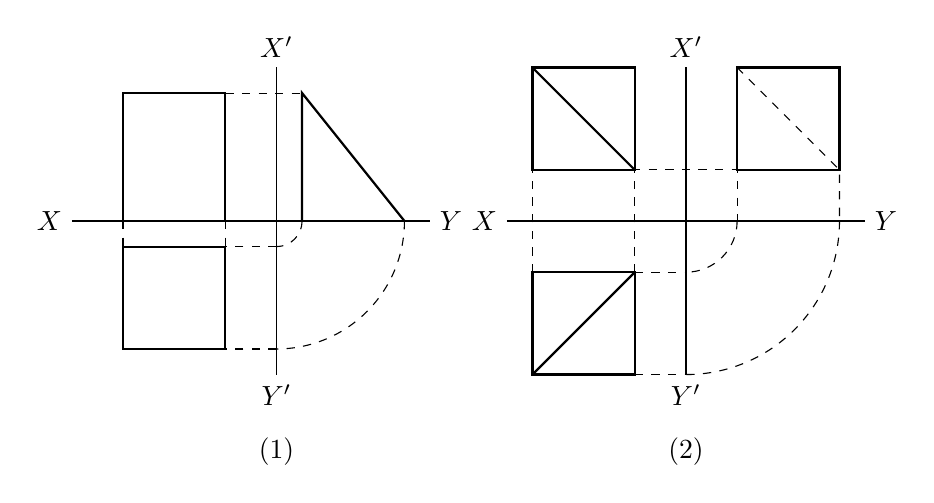
\begin{tikzpicture}[>=latex, scale=.65]
\begin{scope}
\draw(-4,0)node[left]{$X$}--(3,0)node[right]{$Y$};
\draw(0,-3)node[below]{$Y'$}--(0,3)node[above]{$X'$};
\draw[thick](-3,0) rectangle (-1,2.5);
\draw[thick](.5,0)--(.5,2.5)--(2.5,0);
\draw[thick](-3,-.5) rectangle (-1,-2.5);
\draw[dashed](-3,0)--(-3,-.5);
\draw[dashed](-1,0)--(-1,-.5);
\draw[dashed](0,-.5)--(-1,-.5);
\draw[dashed](0,-2.5)--(-1,-2.5);
\draw[dashed](-1,2.5)--(.5,2.5);
\node at (0,-4.5){(1)};
\draw[dashed](.5,0) arc (0:-90:.5);
\draw[dashed](2.5,0) arc (0:-90:2.5);


\end{scope}
\begin{scope}[xshift=8cm]
    \draw(-3.5,0)node[left]{$X$}--(3.5,0)node[right]{$Y$};
    \draw(0,-3)node[below]{$Y'$}--(0,3)node[above]{$X'$};
    \draw[thick](-3,1) rectangle (-1,3);
    \draw[thick](-3,-1) rectangle (-1,-3);
    \draw[thick](3,1) rectangle (1,3);
    \draw[thick](-3,3)--(-1,1);
    \draw[dashed](1,3)--(3,1)--(3,0);
    \draw[thick](-1,-1)--(-3,-3);
    \draw[dashed](-3,-1)--(-3,1);
    \draw[dashed](-1,-1)--(-1,1)--(1,1)--(1,0);
    \draw[dashed](-1,-1)--(0,-1);
    \draw[dashed](-1,-3)--(0,-3);
    \draw[dashed](1,0) arc (0:-90:1);
    \draw[dashed](3,0) arc (0:-90:3);
    \node at (0,-4.5){(2)};
\end{scope}


\end{tikzpicture}
    \caption*{第2题}
\end{figure}

\section*{习题1.1}
\addcontentsline{toc}{subsection}{习题1.1}

\begin{enumerate}
    \item 画出半径为2cm的球的三视图.
    \item 根据二视图,试
    补画出它的左视图,并画视图所表示的立体的直观图.
\begin{figure}[htp]
  \centering
\includegraphics[scale=.4]{fig/ch1-tu2.png}
  \caption*{第2题}
\end{figure}


    \item 试回答下列二视图(1)—(4)中每一个是立
    体直观图(a)—(d)中的哪一个的视图.
    \begin{figure}[htp]
      \centering
    \includegraphics[scale=.5]{fig/ch1-tu3.png}
    \end{figure}
    \begin{figure}[htp]
      \centering
    \includegraphics[scale=.5]{fig/ch1-tu4.png}
      \caption*{第3题}
    \end{figure}
    (注:(2)与(3)中的点划线表示的是该视图所表示的
    立体的轴线及中心线)

    \item 补全下列各视图的投影.
    \begin{figure}[htp]
      \centering
    \includegraphics[scale=.5]{fig/ch1-tu5.png}
    \end{figure}
    \begin{figure}[htp]
      \centering
    \includegraphics[scale=.5]{fig/ch1-tu6.png}
      \caption*{第4题}
    \end{figure}   


    \item 根据三视图,用两种方法画出它们所表示的立体直观图.
    \begin{figure}[htp]
      \centering
    \includegraphics[scale=.5]{fig/ch1-tu7.png}
      \caption*{第5题}
    \end{figure}
    (注:图中尺寸单位为mm)
\end{enumerate}



\section{集合运算}
\subsection{复习}
关于集合的初步知识,我们在初中几何中已经学过了,
现在简要地复习一下要点:

\subsubsection{集合}
通常我们把一些确定的、彼此不同的“事物”
作为一个整体考虑时,便说这个整体是一个\textbf{集合},这些事物叫做该集合的\textbf{元素}.

\begin{blk}{问题1}
    下列集合在空间表示什么图形?
\[\begin{split}
 A&=\{X| OX=5{\rm cm},\; O\text{点是三维空间的一个定点,
$X$是三维空间的点}\}\\
B&=\{P| OP<5{\rm cm},\; O\text{点是三维空间的一个定点,
$P$是三维空间的点}\}\\
C&=\{P| OP>5{\rm cm},\; O\text{点是三维空间的一个定点,
$P$是三维空间的点}\}   
\end{split}\]
\end{blk}

\subsubsection{集合关系}

\paragraph{包含关系}

如果集合$A$中的每一个元素也是集合$B$的元素,则称“$A$包含于$B$”或“$B$包含$A$”,也可以说$A$是$B$的子集.记作$A\subseteq B$, 或$B\supseteq A$. 

若$x\in A$, 则$x\in B$; 但$B$中至少有一个元素$y$不属于$A$, 则称$A$为$B$\textbf{真子集}.记作$A\subset B$或$B\supset A$.


\paragraph{相等关系}

如果两个集合$A,B$由共同的元素构成,我们说这两个集合相等,记作$A=B$. 

判定两个集合相等的方法是:若$A\subseteq B$且$B\subseteq A$, 则$A=B$. 

\begin{blk}{问题2}
    若$A\subset B$且$B\subset A$, 则$A$与$B$是否相等?为什么?
\end{blk}

\paragraph{空集、全集与补集}

不含有任何元素的集合叫做\textbf{空集},用$\emptyset$表示,空集是任何集合的子集.注意空集与零集合不同,零集合包含一个零元素,记作$\{0\}$, 而空集不含有任何元素.

我们把讨论对象所涉及的整个范围称作“全集”,用$I$表示.讨论的范围如果是整数,那么$I$就表示整数集.讨论的范围如果是实数,那么$I$就表示实数集.讨论的是三维空间,则$I$就表示三维空间.

设$A\subset I$, 则集合$\{x|x\in I,\; x\notin A\}$, 称为$A$的\textbf{补集},记作$\sim A$. 也可记作$\overline{A}$.

\begin{blk}{问题3}
\begin{enumerate}
    \item 若$I$为整数集,$A$是偶数集,则$\sim A$为什么
数集?
\item 若$I$为实数集,$A$为无理数集,则$\sim A$为什
么数集?
\end{enumerate}
\end{blk}

\paragraph{集合的“交”与“并”}

由集合$A$和集合$B$的共同元素所组成的集合称作集合$A$与$B$的\textbf{交集}.记作$A\cap B$,即
\[A\cap B=\{x|x\in A\text{ 且 }x\in B\}\]

由集合$A$的元素或集合$B$的元素合并而成的集合叫作$A$和$B$的\textbf{并集},记作$A\cup B$,即
\[A\cup B=\{x|x\in A\; \text{ 或 }\; x\in B\}\]

\begin{blk}{问题4}
    设$A=\{1,a,a^2\}$, $B=\{1,a,b\}$, 假定$a,b$都是实数,并且$A\cap B=\{1, 3\}$, $A\cup B=\{1,a,2a,3a\}$, 求
$a$和$b$的值分别是多少?
\end{blk}


\subsection{集合运算}

我们学过的集合的“交”、“并”、“补”都是集合的运算.

我们学过的数的运算是有算律的,那么集合的运算有什么算律呢?

我们很容易看出以下的事实成立:

\begin{blk}{}
\begin{itemize}
    \item $    A\cap A=A,\qquad     A\cup A=A$
\item $    A\cap I=A,\qquad    A\cup I=I$
\item $    A\cap \emptyset=\emptyset,\qquad  A\cup \emptyset=A$
\item $    A\cap B\subset A \quad \text{且}\quad A\cap B\subset B$
\item $A\subset A\cup B \quad \text{且}\quad B\subset A\cup B$
\item $A\cup \bar{A}=I,\qquad A\cap \bar{A}=\emptyset,\qquad \overline{\bar{A}}=A$    
\end{itemize}
\end{blk}

我们把$A\cap \bar{B}$称作$A$与$B$的\textbf{差集},记作$A-B$, 即
\[A-B=\{x|x\in A \quad \text{且}\quad x\notin B\}\]

差集的维恩图如图1.14所示:
\begin{figure}[htp]
    \centering
\begin{tikzpicture}[scale=1.2]
\begin{scope}
    \draw(-2,0) rectangle (2,3);
\fill[pattern=north east lines](-.65,1.5) circle (.9);
\draw[fill=white](.7,1.5) circle (1);
\draw(-.65,1.5) circle (.9);
\node at (2,0)[above left]{$I$};
\node at (-.65,2.6){$A$};
\node at (.7,2.7){$B$};
\node at (-.9,1.5)[fill=white]{$A-B$};
\node at (0,-.5){(1)};
\end{scope}
\begin{scope}[xshift=5cm]
    \draw(-2,0) rectangle (2,3);
\draw[pattern=north east lines](-.5,1.5) circle (1.2);
\draw[fill=white](-.5,1.8) circle (.5);

\node at (2,0)[above left]{$I$};
\node at (-1,2.8){$A$};
\node at (-.5,1.8){$B$};
\node at (-.5,.8)[fill=white]{$A-B$};
\node at (0,-.5){(2)};
\end{scope}
\begin{scope}[yshift=-4cm]
    \draw(-2,0) rectangle (2,3);
\draw[pattern=north east lines](-.65,1.5) circle (.9);
\draw[fill=white](.9,1.5) circle (.4);
\draw(-.65,1.5) circle (.9);
\node at (2,0)[above left]{$I$};
\node at (-.65,2.6){$A$};
\node at (.9,2.2){$B$};
\node at (-.65,1.5)[fill=white]{$A-B$};
\node at (0,-.5){(3)};
\end{scope}
\begin{scope}[xshift=5cm, yshift=-4cm]
    \draw(-2,0) rectangle (2,3)node[below left]{$I$};
    \draw(-.5,1.5) circle (1.2);
    \draw(-.5,1.8) circle (.5);
\node at (2,0)[above left]{$A-B=\emptyset$};
\node at (-.5,1.8){$A$};
\node at (-.5,1){$B$};
\node at (0,-.5){(4)};
\end{scope}
\end{tikzpicture}
    \caption{}
\end{figure}

\begin{blk}
    {问题1}设$A=\{\text{等腰三角形}\}$,$B=\{\text{直角三角形}\}$,
    则$A-B$是由什么三角形组成的集合?
\end{blk}


\begin{blk}
     {问题2}如果$A$为有理数的集合,$B$为非负有理数的集合,
    那么$A-B$是什么集合?
\end{blk}

\begin{blk}
     {问题3}设$I$为全集,$A$为$I$的一个子集,则$I-A$是个什么集
    合?(参看下面的维恩图思考)
\end{blk}

由问题3可知:
\[I-A=I\cap \bar A=\bar A\]

由此可见:补集可以看作差
集的特殊情况.

\begin{figure}[htp]
    \centering
\begin{tikzpicture}
\draw[pattern= north east lines](0,3) rectangle (4,0)node[above left, fill=white]{$I$};
\draw[fill=white](2,1) circle (.7);
\node at (2,1){$A$};
\node at (2,2.5)[fill=white]{$I-A$};
\end{tikzpicture}
    \caption{}
\end{figure}


集合的交集、并集和差集三
种运算很类似于数的乘法、加法
和减法,例如在数的计算中有
\[3\x2=2\x 3,\qquad 3+2=2+3\] 
在集合的运算中相应地有\[A\cap B=B\cap A,\qquad  A\cup B=B\cup A\]
在数的计算中有:
\[3\x(2\x4)=(3\x2)\x4,\qquad 3+(2+4)=(3+2)+4\]
在集合的运算中相应地有
\[A\cap (B\cap C)=(A\cap B)\cap C,\qquad 
A\cup (B\cup C)=(A\cup B)\cup C\]
这由维恩图很容易直观地看出
来.我们把它们所具有的一些算律归结为如下定理:

\begin{blk}
{定理} 集合的交与并满足以下算律
\begin{enumerate}
\item 结合律:
\[\begin{split}
     (A\cap B)\cap C=A\cap (B\cap C)&\qquad \text{(交的结合律)}\\
     (A\cup B)\cup C=A\cup (B\cup C)&\qquad \text{(并的结合律)}
\end{split} \]
\item 交换律:
\[\begin{split}
    A\cap B=B\cap A&\qquad \text{(交的交换律)}\\
    A\cup B=B\cup A&\qquad \text{(并的交换律)}
\end{split} \]
\end{enumerate}
\end{blk}

\begin{proof}
    我们只证“并的结合律”,其余类似地由同学们
    自己证明.
\[\begin{split}
     x\in (A\cup B)\cup C &\quad \Rightarrow \quad x\in (A\cup B)\; \text{ 或 }\;  x\in C\\
     &\quad \Rightarrow \quad  (x\in A \; \text{ 或 }\;  x\in B)\; \text{ 或 }\;  x\in C  \\
     &\quad \Rightarrow \quad   x\in A\; \text{ 或 }\;  (x\in B\; \text{ 或 }\;  x\in C) \\
     &\quad \Rightarrow \quad  x\in A\; \text{ 或 }\;  x\in (B\cup C) \\
     &\quad \Rightarrow \quad  x\in A\cup (B\cup C)  
\end{split}\]
$\therefore\quad (A\cup B)\cup C\subseteq A\cup (B\cup C)$

同理可证:$A\cup (B\cup C)\subseteq (A\cup B)\cup C$

$\therefore\quad (A\cup B)\cup C=A\cup (B\cup C)$
\end{proof}

\begin{blk}
  {定理} 对于补集有以下法则成立(德·摩根法则)
\begin{enumerate}
  \item $ \overline{A\cap B}=\bar A\cup\bar B$
  \item $\overline{A\cup B}=\bar A\cap \bar B$
\end{enumerate}
\end{blk}

\begin{proof}
\begin{enumerate}
  \item \[\begin{split}
    x\in \overline{A\cap B} & \quad \Longleftrightarrow\quad x\notin A\cap B\\
    & \quad \Longleftrightarrow\quad \text{若$x\in A$则$x\notin B$,\quad 若$x\in B$则$x\notin A$}\\
    & \quad \Longleftrightarrow\quad x\notin A\text{ 或 }x\notin B\\
    & \quad \Longleftrightarrow\quad x\in\bar{A}\text{ 或 }x\in\bar{B}\\
    & \quad \Longleftrightarrow\quad x\in\left(\bar{A}\cup\bar{B}\right)\\
  \end{split}\]

 $\therefore\quad \overline{A\cap B}=\bar A\cup\bar B$ 
  \item 类似地可以证明2式.
\end{enumerate}
\end{proof}

\begin{blk}
  {定理} 对于三个集合$A$、$B$、$C$, 有以下分配律成立
\begin{enumerate}
  \item 交对并的分配律:$A\cap (B\cup C)=(A\cap B)\cup(A\cap C)$
  \item 并对交的分配律:$A\cup(B\cap C)=(A\cup B)\cap (A\cup C)$
\end{enumerate}
\end{blk}

\begin{proof}
  同学们可用定义证明1, 这里我们仅利用1和德·摩根法则证2.
\[\begin{split}
    \overline{A \cup(B \cap C)} &=\bar{A} \cap(\overline{B \cap C}) \\
    &=\bar{A} \cap(\bar{B} \cup \bar{C}) \\
    &=(\bar{A} \cap \bar{B}) \cup(\bar{A} \cap \bar{C}) \\
    &=\overline{A \cup B} \cup \overline{A \cup C} \\
    &=\overline{(A \cup B) \cap(A \cup C)}
\end{split}\]
对上式两端取补集,据$\overline{\bar A}=A$, 则有:
\[A\cup (B\cap C)=(A\cup B) \cap (A\cup C)\]
\end{proof}

\begin{example}
  设$A$、$B$、$C$、$D$都是集合,证明:
\[A\cap (B\cup C\cup D)=(A\cap B)\cup (A\cap C)\cup (A\cap D)\]
\end{example}

\begin{proof}
\begin{align*}
  A\cap (B\cup C\cup D)&= A\cap \big(B\cup(C\cup D)\big)  \tag{结合律}\\
  &=(A\cap B)\cup \big(A\cap (C\cup D)\big)  \tag{分配律}\\
  &=(A\cap B)\cup \big((A\cap C)\cup  (A\cap D)\big)\tag{分配律}\\
  &=(A\cap B)\cup (A\cap C)\cup  (A\cap D)  \tag{结合律}
\end{align*}
\end{proof}

\begin{example}
  试用$\bar A$、$\bar B$、$\bar C$表示$\overline{(A\cap B)\cup (B\cap C)}$
\end{example}


\begin{solution}
\begin{align*}
  \overline{(A\cap B)\cup (B\cap C)}&=\overline{(B\cap A)\cup (B\cap C)}  \tag{交换律}\\
  &=\overline{B\cap (A\cup C)} \tag{分配律}\\
  &=\bar B\cup \overline{(A\cup C)} \tag{德·摩根法则}\\
  &=\bar B\cup (\bar A\cap \bar C) \tag{德·摩根法则} 
\end{align*} 
\end{solution}
  


\begin{ex}
\begin{enumerate}
  \item 如果$A=\{\text{过$M$点的圆}\}$,$B=\{\text{过$P$点的圆}\}$. 
那么,求$A\cap B$, $A\cup B$, $\overline{A\cap B}$, $\overline{A\cup B}$.
\item 设$A=\{-3, 1, 2\}$, $B=\{-1, 0, 1\}$, $C=\{-2, 0, 2\}$. 求:
\begin{multicols}{2}
\begin{enumerate}
  \item $(B\cap A)\cup (A\cap C)$
  \item $(B\cup C) \cap A$
\end{enumerate}
\end{multicols}

\item 在下表的空格处填上适当的集合.
\begin{center}
\begin{tabular}{c|ccc}
  \hline
  $\bigcap $ & $\emptyset$ &$A$&$B$ \\
  \hline
  $\emptyset$ \\
$A$\\
$B$\\
\hline
\end{tabular}\qquad 
\begin{tabular}{c|ccc}
  \hline
  $\bigcup $ & $\emptyset$ &$A$&$B$ \\
  \hline
  $\emptyset$ \\
$A$\\
$B$\\
\hline
\end{tabular}
\end{center}


\item 证明:$\overline{A\cup B}=\bar A\cap \bar B$. 
\item 证明:$A\cap (B\cup C)= (A\cap B)\cup  (A\cap C)$.
\item 证明:$A\cup (A\cap B)=A,\quad A\cap  (A\cup B) =A$.
\end{enumerate}
  
\end{ex}

\section*{习题1.2}
\addcontentsline{toc}{subsection}{习题1.2}

\begin{enumerate}
  \item 设集合$I$、$A$、$B$如图,在图上标出$A\cup B$, $A\cap B$, $A-B$.

\begin{figure}[htp]
  \centering
  \begin{minipage}[t]{0.48\textwidth}
  \centering
  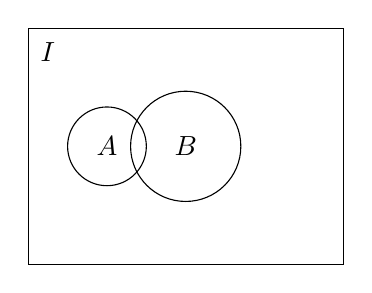
\begin{tikzpicture}[>=latex, scale=1]
\draw(0,0) rectangle (4,3);
\node at (.25,2.7){$I$};
\draw (1,1.5)node{$A$} circle (.5);
\draw(2,1.5)node{$B$} circle(.7);
  \end{tikzpicture}
  \caption*{第1题}
  \end{minipage}
  \begin{minipage}[t]{0.48\textwidth}
  \centering
  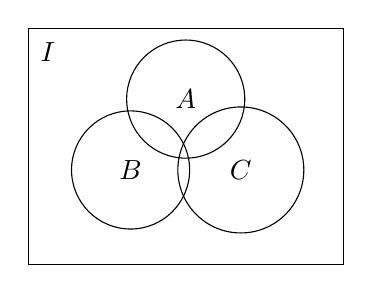
\begin{tikzpicture}[>=latex, scale=1]
\draw(0,0) rectangle (4,3);
\node at (.25,2.7){$I$};
\draw (2,2.1)node{$A$} circle (.75);
\draw(1.3,1.2)node{$B$} circle(.75);
\draw(2.7,1.2)node{$C$} circle(.8);

  \end{tikzpicture}
  \caption*{第2题}
  \end{minipage}
\end{figure}


  \item 设集合$I$、$A$、$B$、$C$, 如图所示,用阴影表示出下列集合:
\begin{multicols}{2}
\begin{enumerate}
  \item $\overline{A\cup B\cup C}$
  \item $\bar A\cup \bar C$
  \item $\overline{A\cap B}\cap C$
  \item $(A\cap B)\cup C$
  \item $(A-B)\cup C$
  \item $A-(B\cup C)$
  \item $A-(\bar B\cup \bar C)$
\end{enumerate}
\end{multicols}

\item   设$A$、$B$、$C$、$D$、$E$都是集合,试用结合律,分配律证明:
\[A\cap  (B\cup C\cup D\cup E)=(A\cap B)\cup (A\cap C)\cup (A\cap D)\cup (A\cap E)\] 
\item 若$A\cup B=A\cup C$, 问$B=C$是否成立?又若$A\cap B=A\cap C$且$A\ne \emptyset$, 问$B=C$是否成立,为什么?
\item 从下面的关系中,可以得到什么结论?为什么?
\begin{multicols}{2}
\begin{enumerate}
  \item $A\subseteq B$且$B\subseteq A$
  \item $R\subseteq S$且$T\subseteq R$
  \item $A\subseteq B$且$B\subseteq C$
  \item $X\subseteq G$, $Y\subseteq T$且$T\subset X$
  \item $A\subseteq Q$, $Q\subseteq R$且$R\subseteq A$
  \item $P\subseteq Q$且$R\subseteq Q$
\end{enumerate}
\end{multicols}

\item 设$A=\{0, 1, 2, 3, 4\}$, $B=\{1, 2, 3\}$, $C=\{1, 4\}$, 
  $D= \{2, 3, 4\}$. 求$(A\cap B)\cup (A\cap C)\cup (A\cap D)$.
\item 用德摩根法则证明:
\[A\cap \overline{B\cap C}=\overline{\bar A\cup B}\cup\overline{\bar A\cup C}\]
\end{enumerate}


\section{平面}

\subsection{平面的表示法}

面有两种,一种是平的面也就是平面,另一种是不平的面,也就是曲面.像平静的水面,门窗的玻璃面等都给人以平面的形象,而像皮球,人脸部的表面都给人以曲面的形象.

我们画一个平面通常用一个平行四边形来表示,在
画水平位置的平面时,通常把平行四边形的一边画成水平,把一个角画成$45^{\circ}$ (或$135^{\circ}$), 平面在空间是无限伸展的.(图1.16)

\begin{figure}[htp]
  \centering
\begin{tikzpicture}[>=latex]
  \tkzDefPoints{0/-.5/A, 2.5/-.5/B, 3.25/1/C}
  \tkzDefPointsBy[translation = from B to C](A){D}
\tkzDrawPolygon(A,B,C,D)
\node at (A)[above right]{$M$};
\foreach \x in {.75,1.25,1.75,2.25,2.75,3.25}
{
  \draw[->](\x,1.2)--(\x+.3, 1.2+.6);
  \draw[->](\x-.75,-.7)--(\x-.75-.3, -.7-.6);
}
\foreach \x in {-.5,0,.5,1}
{
  \draw[->](0+.5*\x, \x)--(0+.5*\x-.5, \x);
  \draw[->](3+.5*\x, \x)--(3+.5*\x+.5, \x);
}

\draw[->](0-.1,-.5-.1)--(0-.6,-.5-.6);
\draw[->](2.5+.1,-.5-.1)--(2.5+.6,-.5-.6);
\draw[->](3.25+.1,1+.1)--(3.25+.6,1+.6);
\draw[->](.75-.1,1+.1)--(.75-.6,1+.6);

\end{tikzpicture}
  \caption{}
\end{figure}

我们通常用一个字母如$M$、$N$、$\pi$、$\alpha$、$\beta$、$\gamma$来表示一个平面,如平面$M$, 平面$\alpha$等,有时也用平行四边形相对的两个顶点表示平面,如平面$AC$ (图1.17(3)), 有时也用平面上不共线三点表示一个平面,如平面$ABC$. 在画平面时,被遮盖
的部分常用虚线表示或不画出来.(图1.17).

\begin{figure}[htp]
  \centering
\begin{tikzpicture}
\begin{scope}
\tkzDefPoints{0/0/A, 1.5/0/B, 1.5/1.5/D, 3/0/C, 3.75/1/C'}
\tkzDefPointsBy[translation= from C to C'](A,B,D){A',B',D'}
\tkzDrawSegments(A,C C',C B',C' D',B' D,D' D,B A,A' B,B')
\tkzInterLL(A',C')(B,D)\tkzGetPoint{T}
\tkzDrawSegments(T,A')
\tkzLabelPoint[above left](C){$M$}
\tkzLabelPoint[right](D){$N$}


\node at (1.5,-1.25){(1)};
\end{scope}
\begin{scope}[xshift=4cm, scale=.7]
  \tkzDefPoints{0/0/A1,4/0/B1,5/1/C1, 4.2/1.75/B2}
    \tkzDefPointsBy[translation= from B1 to C1](A1){D1}
    \tkzDefPointsBy[translation= from B1 to B2](A1,C1,D1){A2,C2,D2}
\tkzDefMidPoint(A1,B1)\tkzGetPoint{E1}
\tkzDefMidPoint(C1,D1)\tkzGetPoint{F1}
\tkzDefMidPoint(A2,B2)\tkzGetPoint{E2}
\tkzDefMidPoint(C2,D2)\tkzGetPoint{F2}
\tkzDefPointWith[linear, K=2](E1,E2) \tkzGetPoint{E3}
\tkzDefPointWith[linear, K=1.7](E2,E1) \tkzGetPoint{E4}
\tkzDefPointWith[linear, K=2](F1,F2) \tkzGetPoint{F3}
\tkzDefPointWith[linear, K=1.7](F2,F1) \tkzGetPoint{F4}

\tkzDrawSegments[thick](A1,B1 B1,C1 D1,A1 A2,B2 B2,C2 D2,A2 E3,E4 E1,F1 E2,F2 E3,F3 F3,F2 F4,E4 F1,C1 F2,C2)
\tkzLabelPoint[above left](B1){$\beta$}
\tkzLabelPoint[above left](B2){$\alpha$}
\tkzLabelPoint[right](E3){$\gamma$}

\tkzInterLL(C1,D1)(E1,E2) \tkzGetPoint{T1}
\tkzInterLL(C2,D2)(E1,E2) \tkzGetPoint{T2}
\tkzDrawSegments[thick](T1,D1 T2,D2)

\tkzInterLL(A1,B1)(F1,F2) \tkzGetPoint{T3}
\tkzInterLL(A2,B2)(F1,F2) \tkzGetPoint{T4}
\tkzDrawSegments[thick](F4,T3 T4,F1)

\node at (2,-2){(2)};
\end{scope}
\begin{scope}[xshift=9cm, scale=.8]
  \tkzDefPoints{0/0/E, .6/.9/B, .2/2.5/A, 3/0/F}
\tkzDefPointsBy[translation= from E to F](A,B){D,C}
\tkzDrawPolygon(A,B,E,F,C,D)
\tkzDrawSegments(C,B)
\tkzDefPointWith[linear,K=1.6](F,C)\tkzGetPoint{b}
\tkzDefPointsBy[translation= from C to b](B){a}
\tkzInterLL(a,b)(C,D)\tkzGetPoint{tmp}
\tkzDrawSegments(tmp,b b,C)
\tkzLabelPoints[left](A,B,E)
\tkzLabelPoints[right](D,F)
\tkzLabelPoints[above left](C)
\node at (1.5,-1.5){(3)};
\end{scope}
\end{tikzpicture}
  \caption{}
\end{figure}


\subsection{点、直线、平面的关系的集合表示法}

\begin{enumerate}
  \item 点$P$在直线$\ell$上(或直线$\ell$过$P$点),记作$P\in\ell$.
  \item 点$P$在平面$\alpha$上(或点$P$在平面$\alpha$内,或平面$\alpha$过$P$点),
记作$P\in\alpha$. 若$P$点不在平面$\alpha$内则$P\notin \alpha$.
\item 直线$\ell$在平面$\alpha$内(或平面$\alpha$包含直线$\ell$, 或平面$\alpha$通过$\ell$),
记作$\ell\subset \alpha$,或$\ell\cap \alpha=\ell$.
\item 直线$\ell$和平面$\alpha$没有公共点.记作$\ell\cap \alpha=\emptyset$.
\item 直线$\ell$和平面$\alpha$有一个公共点$P$ (或直线$\ell$交平面$\alpha$于点$P$), 
记作$\ell\cap \alpha=P$.
\item 平面$\alpha$和平面$\beta$相交于$\ell$, 记作$\alpha\cap \beta=\ell$.
\item 平面$\alpha$和平面$\beta$没有公共线,记作$\alpha\cap \beta=\emptyset$.
\end{enumerate}

\begin{figure}[htp]
  \centering
\begin{tikzpicture}
\begin{scope}
\tkzDefPoints{0/0/A, 3/0/B, 3.5/1.5/C}
\tkzDefPointsBy[translation = from B to C](A){D}
\tkzDrawPolygon(A,B,C,D)
\node at (A)[above right]{$\alpha$};
\tkzDefPoints{2/1/P}
\tkzDrawPoints(P)
\tkzLabelPoints[right](P)
\node at (1.8,-.5) {$P\in \alpha$};


\end{scope}
\begin{scope}[xshift=4cm]
  \tkzDefPoints{0/0/A, 3/0/B, 3.5/1.5/C}
\tkzDefPointsBy[translation = from B to C](A){D}
\tkzDrawPolygon(A,B,C,D)
\node at (A)[above right]{$\alpha$};
\tkzDefPoints{2/2/P}
\tkzDrawPoints(P)
\tkzLabelPoints[right](P)
\node at (1.8,-.5) {$P\notin\alpha$};

\end{scope}
\begin{scope}[xshift=8cm]
  \tkzDefPoints{0/0/A, 3/0/B, 3.5/1.5/C}
\tkzDefPointsBy[translation = from B to C](A){D}
\tkzDrawPolygon(A,B,C,D)
\node at (A)[above right]{$\alpha$};
\node at (1.8,-.5) {$\ell\subset \alpha$};
\draw(.7,1.2)--node[below]{$\ell$}(2.5,.4);

\end{scope}
\begin{scope}[yshift=-3.5cm, xshift=2cm]
  \tkzDefPoints{0/0/A, 3/0/B, 2.5/1.5/C}
\tkzDefPointsBy[translation = from B to C](A){D}
\tkzDrawPolygon(A,B,C,D)
\node at (A)[above right]{$\alpha$};
\tkzDefPoints{2/1/P, 2.5/2.5/P'}
\tkzDrawPoints(P)
\tkzLabelPoints[right](P)
\tkzInterLL(P,P')(A,B)  \tkzGetPoint{P''}
\node at (1.8,-1) {$\ell\cap \alpha=P$};
\tkzDefPointWith[linear, K=2](P',P)\tkzGetPoint{P0}
\tkzDrawSegments(P,P' P'',P0)
\tkzLabelPoint[right](P'){$\ell$}
\end{scope}
\begin{scope}[yshift=-3.5cm,xshift=7cm]
  \tkzDefPoints{0/0/A, 3/0/B, 2.5/1.5/C}
  \tkzDefPointsBy[translation = from B to C](A){D}
  \tkzDrawPolygon(A,B,C,D)
  \node at (1.8,-1) {$\ell\cap \alpha=\emptyset$};
  \draw(-.2,2)--(2.3,2)node[right]{$\ell$};
  \node at (A)[above right]{$\alpha$};

\end{scope}  
\begin{scope}[yshift=-7.5cm, xshift=2cm]
  \tkzDefPoints{0/0/A, 3.5/0/B, 2.5/1/C}
  \tkzDefPointsBy[translation = from B to C](A){D}
 \tkzDrawSegments(A,B B,C D,A)
 \node at (A)[above right]{$\alpha$};
\tkzDefPointWith[linear, K=.4](A,B)  \tkzGetPoint{A'}
\tkzDefPointWith[linear, K=.65](C,D)  \tkzGetPoint{A''}
\tkzDefPoints{2.2/1.5/C'}
\tkzDefPointWith[linear, K=1.4](C',A')  \tkzGetPoint{D'}
\tkzDefPointsBy[translation = from A' to A''](C',D'){C'',D''}
\tkzDrawSegments(A'',C'' C'',C' C',D' D,A'' A',A'')
\tkzInterLL(D',D'')(A,B)  \tkzGetPoint{tmp1}
\tkzDrawSegments(D',tmp1)
\tkzInterLL(D',C')(C,D)  \tkzGetPoint{tmp2}
\tkzDrawSegments(C,tmp2)
\node at (C'')[below]{$\beta$};
\tkzLabelSegment[above](A',A''){$\ell$}
\node at (1.5,-1) {$\alpha\cap \beta=\ell$};



\end{scope}
\begin{scope}[yshift=-7.5cm, xshift=7cm]
  \tkzDefPoints{0/-.5/A, 2.5/-.5/B, 3.25/.5/C}
  \tkzDefPointsBy[translation = from B to C](A){D}
\tkzDrawPolygon(A,B,C,D)
\node at (A)[above right]{$\alpha$};
\tkzDefPoints{0/1/A'}
\tkzDefPointsBy[translation = from A to A'](B,C,D){B',C',D'}
\tkzDrawPolygon(A',B',C',D')
\node at (B')[above left]{$\beta$};
\node at (1.5,-1) {$\alpha\cap \beta=\emptyset$};

\end{scope}

\end{tikzpicture}

  \caption{}
\end{figure}




\subsection{平面的基本性质}

木工在检查木板面是不是“很平”时,通常用直尺沿各个方向来靠紧板面,如果不管怎么靠,中间都不出现间隙,这块板面就是平的.也就是说无论连结平面内怎样的两点的直线,都包含在这个平面内,这就是平面的一条基本性质.

\begin{blk}
  {基本性质1} 如果一条直线上的两点在一个平面内,那么这条直线就被包含在这个平面内.
\end{blk}

如图1.19(1)所示,若点$A\in$平面$\alpha$, 点$B\in$平面$\alpha$, 则直线$AB\subset$平面$\alpha$. 

这时,我们也称直线$AB$在平面$\alpha$内或平面$\alpha$通过直线$AB$. 但在图1.19(2)中,虽然点$A\in$面$\beta$, 点$B\in$面$\beta$, 而直线$AB\not\subset$面$\beta$, 因此面$\beta$不是平面.

\begin{figure}[htp]\centering
  \begin{minipage}[t]{0.48\textwidth}
  \centering
\begin{tikzpicture}
  \tkzDefPoints{0/0/A', 3.5/0/B', 4/2/C'}
\tkzDefPointsBy[translation= from B' to C'](A'){D'}
\tkzDrawPolygon(A',B',C',D')
\node at (A')[above right]{$\alpha$};
\tkzDefPoints{1.5/1.5/A, 2.6/1/B}
\tkzDrawLines[add= .5 and .7](A,B)
\tkzDrawPoints(A,B)
\tkzLabelPoints[below](A,B)

\end{tikzpicture}
  \caption*{(1)}
  \end{minipage}
  \begin{minipage}[t]{0.48\textwidth}
  \centering
\includegraphics[scale=.6]{fig/1-19.png}
  \caption*{(2)}
  \end{minipage}
  \caption{}
  \end{figure}

\begin{blk}
 {基本性质2} 如果两个不同的平面有一公共点,那么它们相交于过这个点的一条直线.(图1.20)
\end{blk}

例如一个长方体相邻的两个面,在长方体的顶点处交于一点,且交于过这个顶点的一条直线.

\begin{figure}[htp]\centering
  \begin{minipage}[t]{0.48\textwidth}
  \centering
\begin{tikzpicture}[>=latex, scale=1]
\tkzDefPoints{0/0/A, 2.5/0/B, 4.5/1/C}
\tkzDefPointsBy[translation= from B to C](A){D}
\tkzDefPoints{-1/1/F}
\tkzDefPointsBy[translation= from A to D](F){E}
\tkzDrawPolygon(A,B,C,D)
\tkzDrawPolygon(A,D,E,F)
\node at (B)[above]{$\beta$};
\node at (F)[right]{$\alpha$};
\node at (D)[above]{$\ell$};
\tkzDefMidPoint(A,D)  \tkzGetPoint{P}
\tkzLabelPoints[below right](P)
\tkzDrawPoints(P)

  \end{tikzpicture}
  \caption*{(1)}
  \end{minipage}
  \begin{minipage}[t]{0.48\textwidth}
  \centering
  \begin{tikzpicture}[>=latex, scale=1]
\tkzDefPoints{0/0/A, 3.5/0/B, 4.5/1/C}
\tkzDefPointsBy[translation= from B to C](A){D}
\tkzDefPoints{1.5/.8/F}
\tkzDefPointsBy[translation= from B to C](F){E}
\tkzDrawPolygon(B,C,E,F)
\tkzDrawSegments(A,B D,A)
\tkzInterLL(C,D)(E,F)  \tkzGetPoint{M}
\tkzDrawSegments(M,D)\tkzDrawSegments[dashed](M,C)
\node at (A)[above right]{$\alpha$};
\node at (E)[below]{$\beta$};
\node at (C)[right]{$\ell$};
\tkzDefMidPoint(B,C)  \tkzGetPoint{P}
\tkzLabelPoints[right](P)
\tkzDrawPoints(P)
  \end{tikzpicture}
  \caption*{(2)}
  \end{minipage}
  \caption{}
  \end{figure}


\begin{blk}
  {基本性质3}经过不在同一直线上三点,有且只有一个平面.(图1.21(1))
\end{blk}
 
这条基本性换个说法就是:“经过不在同一条直线上的任
意三点,可以作一个平面,且只可以作一个平面”,也可以说:“不共线三点确定一个平面”.

例如,一扇门当在门框安上两个合页(如$A$、$B$两个点)门可以自由转动,但再锁上一把锁之后(如$C$点),门就被固定了,这就是利用了上述平面的基本性质.(图1.21(2))

\begin{figure}[htp]
  \centering
  \begin{minipage}[t]{0.48\textwidth}
    \centering
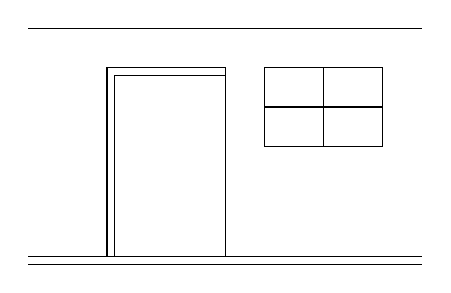
\begin{tikzpicture}[>=latex, scale=1]
\draw(0,0)--(5,0);\draw(0,0.1)--(5,0.1);\draw(0,3)--(5,3);
\draw(1,.1) rectangle(2.5,2.5);
\draw(1.1,.1) rectangle(2.5,2.4);
\draw(1.1,.1) rectangle(2.5,2.4);
\draw(3,1.5) rectangle(4.5,2.5);
\draw(3,2)--(4.5,2);
\draw(7.5/2,1.5)--(7.5/2,2.5);
\tkzDefPoints{1.05/.5/B, 1.05/2/A, 2.5/1.2/C}
\tkzLabelPoints[left](A,B)
\tkzLabelPoints[right](C)
\tkzDrawPoints(A,B,C)
    \end{tikzpicture}
    \caption*{(1)}
    \end{minipage}
    \begin{minipage}[t]{0.48\textwidth}
    \centering
    \begin{tikzpicture}[>=latex, scale=1]
\tkzDefPoints{0/0/A', 3.5/0/B', 4.5/1.8/C'}
\tkzDefPointsBy[translation= from B' to C'](A'){D'}
\node at (A') [above right]{$\alpha$};
\tkzDefPoints{1/.5/B, 2/1.2/A, 3/.4/C}
\tkzDrawPoints(A,B,C)
\tkzLabelPoints[right](A,B,C)
\tkzDrawPolygon(A',B',C',D')

    \end{tikzpicture}
    \caption*{(2)}
    \end{minipage}
  \caption{}
\end{figure}

\begin{blk}
  {推论}
\begin{enumerate}
  \item 一直线与线外一点确定一个平面.
  \item 两条相交直线确定一个平面.
  \item 两条平行直线确定一个平面.
\end{enumerate}
\end{blk}

我们只证明推论1,其余两条同学们自己证明.

\begin{figure}[htp]
  \centering
\begin{tikzpicture}
  \begin{scope}
\tkzDefPoints{0/0/A', 3/0/B', 4/1.5/C'}
\tkzDefPointsBy[translation= from  B' to C'](A'){D'}
\tkzDrawPolygon(A',B',C',D')
\node at (1.5,-.5){(1)};
\tkzDefPoints{1/.25/A, 2.5/.25/B, 2/1.1/C}
\tkzDrawLines[add=.2 and .2](A,B)
\tkzLabelPoints[above](A,B)
\tkzLabelPoints[left](C)
\tkzDrawPoints(A,B,C)
  \end{scope}
  \begin{scope}[xshift=4cm]
    \node at (1.5,-.5){(2)};
\tkzDefPoints{0/0/A', 3/0/B', 4/1.5/C'}
\tkzDefPointsBy[translation= from  B' to C'](A'){D'}
\tkzDrawPolygon(A',B',C',D')
\tkzDefPoints{1.2/.95/A, 3/.95/D, 1/.25/C, 2.75/.25/B}
\tkzDrawSegments(A,B C,D)
\tkzLabelPoints[above](A,B,C,D)
\tkzInterLL(A,B)(C,D)  \tkzGetPoint{E}
\tkzLabelPoints[below](E)
  \end{scope}
  \begin{scope}[xshift=8cm]
    \node at (1.5,-.5){(3)};
\tkzDefPoints{0/0/A', 3/0/B', 4/1.5/C'}
\tkzDefPointsBy[translation= from  B' to C'](A'){D'}
\tkzDrawPolygon(A',B',C',D')
\tkzDefPoints{1.5/.95/A, 3/.95/B, 1/.25/C, 2.5/.25/D}
\tkzDrawSegments(A,B C,D)
\tkzLabelPoints[above](A,B,C,D)
  \end{scope}
\end{tikzpicture}
  \caption{}
\end{figure}

已知:直线$AB$和点$C\notin AB$.

求证:直线$AB$和点$C$确定一个平面.

\begin{proof}
$\because\quad $经过直线$AB$上的两点$A$、$B$与$C$点可以作一个平面$\alpha$ (基本性质2), 而直线$ABC$平面$\alpha$ (基本性质1)

又$\because\quad $过直线$AB$与点$C$不可能再作第二个平面,否
则与基本性质3矛盾.
\end{proof}

\begin{blk}
  {基本性质4} 空间所有的点不全在一个平面上.
\end{blk}

平面是什么?在直观上是清楚的,知道了平面的基本性质,就对平面的本质有了更深入的了解.在此基础上,我们可以给平面下个定义.

\begin{blk}
  {定义} 具有下列性质的空间的一个点集$\pi$叫做平面.
\begin{enumerate}
  \item $\pi$是空间$V$的一个真子集,即$\pi\subset V$.
  \item 至少存在不共线三点$A$、$B$、$C$属于$\pi$.
  \item 若点$M\in\pi$, 点$N\in\pi$, 则有直线$MN\subset \pi$.
\end{enumerate}
\end{blk}

  有了平面的定义,我们就可以判定空间的一个点的集合是否是平面了.

  \begin{example}
设集合$A=\{x|ox=4{\rm cm},\; \text{$o$点是空间$V$的一个定点}\}$,试问$A$是否是平面? 
  \end{example}

  \begin{solution}
如图1.23所示,
\begin{enumerate}
\item $A$显然是空间$V$的一个真子集,
即$A\subset V$因为$O\in V$, 而$O\notin A$.
\item 在$A$上任取不同的三点$P,Q,
R$, 它们一定不共线.
\item 若$M$点$\in A$, $N$点$\in A$, 但直
线$MN\not\subset A$. 
\end{enumerate}

因为$\triangle OMN$是等腰三角形,在底边$MN$上取一点$P$, 连$OP$, 将有
$\angle OPN> \angle OMP$,但$\angle OMP=\angle ONP$
  
$\therefore\quad \angle OPN>\angle ONP$

$\therefore\quad ON>OP$

$\therefore\quad P\notin A$\footnote{如果$MN$过$O$点,则$O\notin A$.} 
  \end{solution}

\begin{figure}[htp]
  \centering
  \begin{minipage}[t]{0.48\textwidth}
  \centering
  \begin{tikzpicture}[>=latex, scale=.8]
\draw[thick](0,0) circle(2);
\draw[dashed](0,0) ellipse[x radius=2, y radius=.5];
\draw (2,0) arc [start angle=0, end angle =-180, x radius=2, y radius=.5];
\tkzDefPoints{.5/-.48/M, 1.5/.3/N, 0/0/O}
\tkzDefMidPoint(M,N)  \tkzGetPoint{P}
\tkzDefPointWith[linear, K=2](M,N) \tkzGetPoint{N'}
\tkzDefPointWith[linear, K=3](N,M) \tkzGetPoint{M'}
\tkzDrawSegments(M,M' N,N')
\tkzDrawSegments[dashed](O,N O,M M,N O,P)

\tkzLabelPoints[right](P)
\tkzLabelPoints[above left](N)
\tkzLabelPoints[below right](M)
\tkzDefPoint(135:2){A}
\tkzLabelPoints[left](O,A)
\tkzDrawPoints(O,A,M,N,P)
  \end{tikzpicture}
  \caption{}
  \end{minipage}
  \begin{minipage}[t]{0.48\textwidth}
  \centering
  \begin{tikzpicture}[>=latex, scale=1]
\tkzDefPoints{0/0/A', 4.5/0/B', 5.5/2.5/C'}
\tkzDefPointsBy[translation= from  B' to C'](A'){D'}
\tkzDrawPolygon(A',B',C',D')
\node at (A')[above right]{$\pi$};
\tkzDefPoints{1.5/.5/A, 4/1.2/C, 2.5/2/B}
\tkzDrawLines[add=.25 and .25](A,B B,C C,A)
\tkzLabelPoints[left](B)
\tkzLabelPoints[below](A,C)
\tkzLabelPoint[above right](B){$\ell_2$}
\tkzLabelPoint[below right](C){$\ell_3$}
\tkzLabelPoint[above left](A){$\ell_1$}

  \end{tikzpicture}
  \caption{}
  \end{minipage}
\end{figure}

  
\begin{example}
两两相交且不过同一点的三条直线必在同一平面内.(图1.24)

已知:直线$\ell_1,\ell_2,\ell_3$且$\ell_1\cap\ell_2=A$, $\ell_2\cap \ell_3=B$, $\ell_1\cap \ell_3=C$.

求证:直线$\ell_1,\ell_2,\ell_3$共面.
\end{example}

  \begin{proof}
$\because\quad \ell_1\cap\ell_2=A$

$\therefore\quad \ell_1$和$\ell_2$确定一个平面$\pi$

$\because\quad B\in\ell_2,\quad  C\in\ell_1$

$\therefore\quad \ell_3\subset$平面$\pi$

$\therefore\quad \ell_1,\ell_2, \ell_3\subset \pi$

即$\ell_1,\ell_2,\ell_3$共面.
  \end{proof}

\begin{example}
顺次连结不在同一平面上的四个点所成的四边形为空间四边形.设有空间四边形$ABCD$, $E,F,G,H$分别是$AB$, $BC$, $CD$和$DA$上的点,如果$EH$和$FG$的延长线交于$P$点,求证:$P$点在空间四边形的对角线$BD$所在的直线上.(图1.25)
\end{example}

\begin{figure}[htp]
  \centering
\begin{tikzpicture}
  \tkzDefPoints{0/0/A', 4.5/0/B', 5.5/2.5/C'}
  \tkzDefPointsBy[translation= from  B' to C'](A'){D'}
  \node at (A')[above right]{$\pi$};
\tkzDrawSegments(A',B' B',C' D',A')
\tkzDefPoints{1/1.2/B, 4/.5/C, 2.5/1.6/D, 2.7/4/A}
\tkzDrawPolygon(A,B,C,D)
\tkzDefPointWith[linear, K=.65](B,A)\tkzGetPoint{E}
\tkzDefPointWith[linear, K=.65](B,C)\tkzGetPoint{F}
\tkzDefPointWith[linear, K=.5](D,A)\tkzGetPoint{H}
\tkzDefPointWith[linear, K=.5](D,C)\tkzGetPoint{G}
\tkzInterLL(E,H)(F,G)\tkzGetPoint{P}
\tkzDrawSegments(E,P F,P)
\tkzDrawLines[add=0 and .25](B,P)
\tkzInterLL(E,P)(C',D')\tkzGetPoint{tmp1}
\tkzInterLL(C',D')(A,B)\tkzGetPoint{tmp2}

\tkzDrawSegments(C',tmp1 D',tmp2)
\tkzDrawSegments[dashed](tmp1,tmp2)
\tkzLabelPoints[below](B,F,C)
\tkzLabelPoints[above](A,P)
\tkzLabelPoints[right](H,G)
\tkzLabelPoints[left](E)
\tkzLabelPoints[above left](D)
\end{tikzpicture}
  \caption{}
\end{figure}

\begin{proof}
$\because\quad A$、$B$、$D$三点不共线,

$\therefore\quad $过$A$、$B$、$D$三点可以确定一个平面$ABD$.

同理,过$C$、$B$、$D$三点可以确定一个平面$CBD$. 并且,平面$ABD\cap $平面$CBD=BD$

又$\because\quad E,H\in$平面$ABD$

$\therefore\quad EH\subset $平面$ABD$

同理$\because\quad F,G\in$平面$CBD$

$\therefore\quad FG\subset $平面$CBD$

$\because\quad EH\cap FG=P$

$\therefore\quad P\in $平面$ABD$且$P\in$平面$CBD$

$\therefore\quad P\in BD$.

即:$P$点在空间四边形$ABCD$的对角线$BD$所在的直线上.
\end{proof}

\begin{figure}[htp]
  \centering
  \begin{tikzpicture}[>=latex, scale=.8]
\begin{scope}
\tkzDefPoints{0/0/A', 4/0/B', 5/2/C, 2/1/A, 3.5/1/B}
\tkzDefPointsBy[translation= from B' to C](A'){D}
\tkzDrawPolygon(A',B',C,D)
\tkzLabelPoint[above right](A'){$\pi$}
\tkzDrawLines[add=0 and 1](A,B)
\tkzLabelPoints[above](A,B)
\tkzDrawPoints(A,B)
\node at (2,-.5){(a)};
\end{scope}
\begin{scope}[xshift=8cm]
  \tkzDefPoints{-.5/0/A', 3.5/0/B', 4.3/1.5/C}
  \tkzDefPointsBy[translation= from B' to C](A'){D}
\tkzDrawSegments(A',B' B',C D,A')
  \tkzLabelPoint[above right](A'){$\alpha$}
  \tkzDefPoints{2/.8/P, 3.3/2.5/A, 2.2/3.5/B}
  \tkzDefPointsBy[translation= from A to B](P){C'}
  \tkzDrawPolygon(A,B,C',P)
\tkzLabelPoints[right](P)
\tkzInterLL(C,D)(P,A)   \tkzGetPoint{tmp1}
\tkzInterLL(C,D)(P,C') \tkzGetPoint{tmp2}
\node at (2,-.5){(b)};
\tkzDrawSegments(C,tmp1 tmp2,D)
\tkzLabelPoint[below](B){$\beta$}



\end{scope}
  \end{tikzpicture}
  \caption*{第1题}
\end{figure}


\begin{ex}
\begin{enumerate}
  \item 下图的画法正确吗?
\begin{enumerate}
  \item 直线$AB$不在平面$\pi$内.
  \item 平面$\alpha$和平面$\beta$只有一个公共点$P$.
\end{enumerate}

\item 画两个平面$M,N$, 满足下列条件:$M\cap N=\emptyset$, 并且
  $a\subset M$, $b\subset M$, $a\cap b=A$, $c\subset N$,$d\subset N$, $c\cap d=\emptyset$.
  \item 
\begin{enumerate}
  \item 画两个相交平面,并在图上标出表示平面的字母.
  \item 画三个平面,使得它们两两相交,但三个平面不共线,
  并在图上标注表示各个平面的字母.
\end{enumerate}  
  \item 一点能不能确定一个平面?二个点呢?三个点呢?怎样的
  三点才能确定一个平面?
  \item 任意一点和一条直线能否确定一个平面?一个点和一条直线在怎样的位置关系时,才能确定一个平面?
  \item 怎样用两条细绳来检查桌子的四个脚的下端是不是在同一
  个平面内.
  \item 设直线$\ell\subset$平面$\alpha$, $A\in\alpha$, $A\notin \ell$, 那么过$A$点画一条直线$AB$, 则直线$AB\subset $平面$\alpha$, 为什么?
  \item 一条直线过平面内一点与平面外一点,它和这个平面有几
个公共点?为什么?
\item 经过同一点的三条直线最多可以确定几个平面?
经过同一点的四条直线最多可以确定几个平面?……经过同一点的$n$条直线最多可以确定多少个平面?
\end{enumerate}
\end{ex}


\section*{习题1.3}
\addcontentsline{toc}{subsection}{习题1.3}

\begin{enumerate}
  \item 设有直线$a,b,c$, $a\cap b=\emptyset$, $a\cap c=A$, $b\cap c=B$, 那么
直线$a,b,c$是否在同一平面内?为什么?
\item 三角形、平行四边形、梯形是否一定是平面图形?为什
么?
\item 用语言叙述下列符号所表示的关系,并画出图形.
\begin{enumerate}
  \item $\ell\subset \pi$
  \item $B\notin \pi,\; B\in \ell$且$\ell\cap\pi=A$
  \item $\ell_1\cap \ell_2=P$且$\ell_1,\ell_2\subset \pi$
  \item $\pi_1\cap \pi_2=\ell,\; \ell'\subset \pi_1$且$\ell\cap \ell'=A$
\end{enumerate}


\item 将下列命题改成语言表述,判断它们是否正确,并说明
理由.
\begin{enumerate}
  \item 当$A\in \pi$, $B\notin \pi$时,线段$AB\subset \pi$.
  \item $A\in\pi,\; B\in\pi,\; C\in AB\quad \Rightarrow\quad C\in\pi $
\end{enumerate}

\item 
\begin{enumerate}
  \item 不共面的四点,可以确定几个平面?
  \item 不共点且两两相交的三条直线可以确定几个平面?
  \item 不共点且两两相交的四条直线可以确定几个平面?
\end{enumerate}

\item 两个不重合的平面,如果有两个公共点$A,B$, 那么其他
的公共点一定在直线$AB$上,为什么?
\item 过直线$\ell$外一点$P$, 与$\ell$上三点$A,B,C$分别画三条直线,证明:直线$PA$, $PB$, $PC$在同一个平面内.
\item 画出图中过$A$、$B$、$C$三点的平面与其他平面的交线.
\begin{figure}[htp]
  \centering
  \begin{minipage}[t]{0.48\textwidth}
    \centering
\begin{tikzpicture}[>=latex, scale=1]
\tkzDefPoints{0/0/a, 3/0/b, 4.5/1/c, 3.5/2.5/e}
\tkzDefPointsBy[translation = from b to c](a){d}
\tkzDefPointsBy[translation = from c to e](d){f}
\tkzDrawPolygon(a,b,c,d)
\tkzDrawPolygon(c,d,f,e)
\tkzLabelPoint[above right](a){$\alpha$}
\tkzLabelPoint[below right](f){$\beta$}
\tkzDefPoints{2/1/A, 3/.5/C, 3.3/2/B}
\tkzDrawPoints(A,B,C)
\tkzLabelPoints[left](B,C)
\tkzLabelPoints[above](A)
    \end{tikzpicture}
    \caption*{(1)}
    \end{minipage}
    \begin{minipage}[t]{0.48\textwidth}
    \centering
    \begin{tikzpicture}[>=latex, scale=1]
\tkzDefPoints{0/0/a, 3/0/b, 3/1.8/c}
\tkzDefPointsBy[translation = from b to c](a){d}
\tkzDrawPolygon(a,b,c,d)
\tkzDefPoints{2/-1/e}
\tkzDefPointsBy[translation = from b to e](a,d){a',d'}
\tkzDrawPolygon(a,b,e,a')\tkzDrawPolygon(d,a,a',d')
\tkzLabelPoint[above left](e){$\pi_2$}
\tkzLabelPoint[right](d'){$\pi_1$}
\tkzLabelPoint[below left](c){$\pi_3$}
\tkzDefPoints{2/0/C, 0/.8/A}
\tkzDefMidPoint(a,a') \tkzGetPoint{B}
\tkzDrawPoints(A,B,C)
\tkzLabelPoints[right](A)
\tkzLabelPoints[above](C)
\tkzLabelPoints[left](B)


    \end{tikzpicture}
    \caption*{(2)}
    \end{minipage}
  \caption*{第8题}
\end{figure}
\end{enumerate}

\subsection{实验与观察:对正方体中线面关系的观察}

用铁丝或细木棍作一个正方体框架,然后对下面各组问
题进行观察研究,自己发现结论.

\begin{enumerate}
  \item 直线与直线位置关系的观察.
\begin{enumerate}
  \item 在正方体$ABCD-A_1B_1C_1D_1$
  内,若$AA_1\parallel BB_1$, $AA_1\parallel DD_1$, 则$BB_1$和
  $DD_1$有什么关系?
 \item 在正方体$ABCD-A_1B_1C_1D_1$
  内,若平面$AC\cap $平面$AB_1=AB$, 
  平面$A_1C_1\cap $平面$AB_1=A_1B_1$并且平
  面$AC\cap $平面$A_1C_1=\emptyset$, 则$AB$和$A_1B_1$有什么关系?
  \item 在正方体$ABCD-A_1B_1C_1D_1$内,若$AB\bot BC$, $AB\bot 
  BB_1$, $A_1B_1\bot BB_1$, $A_1B_1\bot B_1C_1$, 则$AB$和$A_1B_1$有什么关系?
  \item 在正方体$ABCD-A_1B_1C_1D_1$内,若$AD\bot AA_1$, $AA_1\parallel
  BB_1$, 则$AD$与$BB_1$有什么关系?
  \item 在正方体$ABCD-A_1B_1C_1D_1$内,$BB_1\bot A_1B$, $BB_1\bot 
  B_1C_1$且$A_1C_1\bot B_1D_1$, 则$BD_1$与$A_1C_1$有什么关系?
\end{enumerate}
\begin{figure}[htp]\centering
  \begin{minipage}[t]{0.48\textwidth}
  \centering
\begin{tikzpicture}[>=latex, scale=1]
\tkzDefPoints{0/0/A_1, 3/0/B_1, 4/1/C_1, 0/3/A}
\tkzDefPointsBy[translation = from B_1 to C_1](A_1){D_1}
\tkzDefPointsBy[translation = from A_1 to A](B_1,C_1,D_1){B,C,D}
\tkzDrawPolygon(A,B,C,D)
\tkzDrawSegments(A_1,B_1 B_1,C_1 A,A_1 B,B_1 C,C_1)
\tkzDrawSegments[dashed](A_1,D_1 D_1,C_1 D,D_1 D_1,B_1 A_1,C_1 B,D_1)
\tkzLabelPoints[below](A_1,B_1)
\tkzLabelPoints[above](C,D)
\tkzLabelPoints[left](A,D_1)
\tkzLabelPoints[right](C_1,B)


  \end{tikzpicture}
  \caption*{第1题}
  \end{minipage}
  \begin{minipage}[t]{0.48\textwidth}
  \centering
  \begin{tikzpicture}[>=latex, scale=1]
    \tkzDefPoints{0/0/A_1, 3/0/B_1, 4/1/C_1, 0/3/A}
\tkzDefPointsBy[translation = from B_1 to C_1](A_1){D_1}
\tkzDefPointsBy[translation = from A_1 to A](B_1,C_1,D_1){B,C,D}
\tkzDrawPolygon(A,B,C,D)
\tkzDrawSegments(A_1,B_1 B_1,C_1 A,A_1 B,B_1 C,C_1 A,C B,D)
\tkzDrawSegments[dashed](A_1,D_1 D_1,C_1 D,D_1 D_1,B_1 A_1,C_1)
\tkzLabelPoints[below](A_1,B_1)
\tkzLabelPoints[above](C,D)
\tkzLabelPoints[left](A,D_1)
\tkzLabelPoints[right](C_1,B)
  \end{tikzpicture}
  \caption*{第2题}
  \end{minipage}
  \end{figure}

\item 直线与平面位置关系的观察.
\begin{enumerate}
  \item 在正方体$ABCD-A_1B_1C_1D_1$中,若$A_1B_1\subset$平面$A_1C_1$, 
  $AB\parallel A_1B_1$, 则$AB\cap $平面$A_1C=?$
  \item 在正方体$ABCD-A_1B_1C_1D_1$内,若平面$AC\cap $
  平面$B_1D_1=\emptyset$, 则$AC\cap $平面$B_1D_1=?$ $BD\cap $平面$A_1C_1=?$
  \item 在正方体$ABCD-A_1B_1C_1D_1$中,若$DD_1\bot A_1D_1$, 
  $DD_1\bot D_1C_1$, 则$DD_1$和平面$D_1B_1$有什么关系?
  \item 在正方体$ABCD-A_1B_1C_1D_1$中,如果$DC\parallel A_1B_1$, 
  $A_1B_1\bot BB_1$, $A_1B_1\bot B_1C_1$, 则$DC$和平面$BC_1$有什么关系?
\end{enumerate}

\item 平面与平面位置关系的观察.
\begin{enumerate}
  \item 在正方体$ABCD-A_1B_1C_1D_1$中,若$AC\parallel A_1C_1$, 
  $BD\parallel B_1D_1$且$AC\cap BD=O$, $A_1C_1\cap B_1D_1=O'$, 则平面$AC\cap$
  平面$A_1C_1=?$
  \item 在正方体$ABCD-A_1B_1C_1D_1$中,若$AC\cap$平面$A_1C_1
  =\emptyset$, $BD\cap $ 平面$A_1C_1=\emptyset$ 且$AC\cap BD=O$, 则平面$AC\cap $平
  面$A_1C_1=?$
  \item 在正方体$ABCD-A_1B_1C_1D_1$中,若$AO\bot BD$, $AO\bot 
  OO'$且$AO\subset $平面$AO'$, 则平面$AO'$和平面$DO'$有什么关
  系?
\end{enumerate}

\begin{figure}[htp]
  \centering
  \begin{tikzpicture}[>=latex, scale=1]
    \tkzDefPoints{0/0/A_1, 3/0/B_1, 4/1/C_1, 0/3/A}
\tkzDefPointsBy[translation = from B_1 to C_1](A_1){D_1}
\tkzDefPointsBy[translation = from A_1 to A](B_1,C_1,D_1){B,C,D}
\tkzDrawPolygon(A,B,C,D)
\tkzDrawSegments(A_1,B_1 B_1,C_1 A,A_1 B,B_1 C,C_1 A,C B,D)
\tkzDrawSegments[dashed](A_1,D_1 D_1,C_1 D,D_1 D_1,B_1 A_1,C_1)

\tkzInterLL(B,D)(A,C) \tkzGetPoint{O}
\tkzInterLL(B_1,D_1)(A_1,C_1) \tkzGetPoint{O'}
\tkzLabelPoints[below](A_1,B_1,O')
\tkzLabelPoints[above](C,D,O)
\tkzLabelPoints[left](A,D_1)
\tkzLabelPoints[right](C_1,B)
\tkzDrawSegments[dashed](O,O')

  \end{tikzpicture}
  \caption*{第3题}
\end{figure}

\end{enumerate}

通过对正方体的线面位置关系的察观与思考,你能就上
述三组问题中的每个小题,得到一个一般性的命题吗?

\section{直线与直线的位置关系}
\subsection{空间两条直线的位置关系}
在上一节的最后我们对正方体中的线、面关系作了观
察.从观察中发现空间直线与直线有各种不同的位置关系.
在现实生活中也是一样,例如我们观察教室中的各种“直
线”,你会发现,下垂的两条电灯线是互相平行的;黑板相
邻两边是相交的;垂直于地板的一条桌腿与黑板的一条水平
边缘既不相交,也不平行,它们不在同一个平面内.

我们把不在同一平面内的两条直线叫作\textbf{异面直线}.如图
1.26的(1)、(2)中的直线$a$、$b$表示的都是异面直线.

\begin{figure}[htp]
  \centering
\begin{tikzpicture}
\begin{scope}
  \tkzDefPoints{0/0/a,3/0/b,4/1.5/c}
\tkzDefPointsBy[translation = from b to c](a){d}
\tkzDrawPolygon(a,b,c,d)
\tkzLabelPoint[above right](a){$M$}
\tkzDefPoints{1.5/2/B, 2/1/A}
\draw(1,.6)--(3,.6)node[right]{$b$};
\tkzInterLL(A,B)(a,b)\tkzGetPoint{tmp1}
\tkzDefPointWith[linear,K=3](B,A)\tkzGetPoint{D}
\tkzDrawSegments(D,tmp1)
\tkzLabelPoint[above](B){$a$}
\tkzLabelPoints[right](A)
\node at (2,-1.5){(1)};
\tkzDrawSegments(A,B)

\end{scope}
\begin{scope}[xshift=6cm]
  \tkzDefPoints{0/-.8/A,3/-.8/B,4/0.5/B', -1/.7/C}
  \tkzDefPointsBy[translation = from B to B'](A,C){A',C'}
\tkzDrawPolygon(C,A,B,B',A',C')
\tkzLabelPoint[right](C){$M$}
\tkzLabelPoint[above right](A){$N$}
\tkzDrawSegments(A,A')
\draw(0,1)--node[right]{$a$}(0,0);
\draw(1.5,-.2)--node[above]{$b$}(3,-.2);


\node at (1,-1.5){(2)};

\end{scope}
\end{tikzpicture}
  \caption{}
\end{figure}

空间的两条直线有如下的位置关系:
\subsubsection{在同一个平面内}
\begin{enumerate}
\item 相交直线——只有一个公共点.
\item 平行直线——没有公共点.
\item 重合直线.
\end{enumerate}

当两条平行直线中的一条,在保持与另一条直线平行的
条件下无限接近另一条直线时,结果两条平行直线必然重
合.因此,我们把两条直线重合看成是两条直线平行的极限
情况.因此,当我们说两条直线平行时,不排除重合这一极
限情况;当我们说两条相异直线平行时,这就排除了重合的
可能性.

\subsubsection{不在同一个平面内}
异面直线——没有公共点.
如果使用集合语言,上述空间两条直线的位置关系可以
定义如下:

\begin{blk}{定义}
\begin{enumerate}
  \item  空间两条直线$\ell_1$和$\ell_2$相交$\Longleftarrow\ell_1\cap\ell_2=P$
  ($P$是$\ell_1$与$\ell_2$的唯一公共点)
  \item  空间两条直线$\ell_1$和$\ell_2$平行($\ell_1\parallel \ell_2$)$\Longleftarrow \ell_1$和$\ell_2$
  共面且$\ell_1\cap\ell_2=\emptyset$或$\ell_1=\ell_2$(重合)
  \item  空间两条直线$\ell_1$和$\ell_2$异面$\Longleftarrow \ell_1$和$\ell_2$不共面.
\end{enumerate}
\end{blk}

\begin{blk}{问题1}
  下图中,如果$a\parallel b$, $a\subset M$, $b\subset N$, 那么$a,b$是异面
直线吗?
\end{blk}

\begin{center}
\begin{tikzpicture}
\begin{scope}
\tkzDefPoints{0/0/A, 2/0/B, 3.5/1.5/C, -.5/1.2/A'}
\tkzDefPointsBy[translation= from A to A'](B,C,D){B',C',D'}
\tkzDrawPolygon(A,B,C,C',B',A')
\tkzDrawSegments(B,B')
\tkzLabelPoint[above right](A){$M$}
\tkzLabelPoint[above](B){$N$}
\tkzDefPoints{.5/1/a, .85/.2/b, 2.4/1.8/a'}
\tkzDefPointsBy[translation= from a to a'](b){b'}
\tkzDrawSegments(a,b a',b')
\tkzLabelSegment[right](a,b){$a$}
\tkzLabelSegment[left](a',b'){$b$}

\end{scope}
\begin{scope}[xshift=6cm]
  \tkzDefPoints{0/0/A_1, 3/0/B_1, 4/1/C_1, 0/2/A}
\tkzDefPointsBy[translation = from B_1 to C_1](A_1){D_1}
\tkzDefPointsBy[translation = from A_1 to A](B_1,C_1,D_1){B,C,D}
\tkzDrawPolygon(A,B,C,D)
\tkzDrawSegments(A_1,B_1 B_1,C_1 A,A_1 B,B_1 C,C_1)
\tkzDrawSegments[dashed](A_1,D_1 D_1,C_1 D,D_1)
\tkzLabelPoints[below](A_1,B_1)
\tkzLabelPoints[above](C,D)
\tkzLabelPoints[left](A,D_1)
\tkzLabelPoints[right](C_1,B)

\end{scope}
\end{tikzpicture}
\end{center}

\begin{blk}{问题2}
  长方体$ABCD-A_1B_1C_1D_1$中,$AD$棱与哪些棱成异面直线?$AB$棱与哪些棱成异面直线?
$AA_1$棱与哪些棱成异面直线?
\end{blk}

\subsection{平行于同一条直线的二条直线}
“如果三条直线$a,b,c$中,
$a\parallel c$, $b\parallel c$, 那么$a\parallel b$” 当$a$、$b$、$c$共面
时是成立的,如果$a,b,c$不共面时,这个命题是否还成立呢?

\begin{blk}
  {定理} 平行于第三条直线的两条直线互相平行.
\end{blk}

已知:如图1.27不在同一平面上的三条直线$a,b,c$中,
$a\parallel b$, $c\parallel b$. 

求证:$a\parallel c$.

\begin{figure}[htp]
  \centering
\begin{tikzpicture}
\tkzDefPoints{0/0/P, 3/0/Q, 1.9/1/Q', 3/2.5/Q''}
\tkzDefPointsBy[translation= from Q to P](Q',Q''){P',P''}
\tkzDefPointWith[linear, K=.7](Q',Q)\tkzGetPoint{R}
\tkzDrawPolygon(P,P',P'',Q'',R)
\tkzDrawSegments[dashed](P',Q' Q',Q'' Q',R)
\tkzDrawSegments(P,Q Q,R P,P'')
\tkzLabelPoints[below](P)
\tkzLabelPoint[above right](P'){$\pi_1$}
\tkzLabelPoint[below right](P'){$\pi_2$}
\tkzLabelPoint[above right](P){$\pi_3$}
\tkzLabelSegment[below](P,Q){$c$}
\tkzLabelSegment[above](P',Q'){$b$}
\tkzLabelSegment[above](P'',Q''){$a$}
\tkzLabelSegment[above](P,R){$c'$}
\end{tikzpicture}
  \caption{}
\end{figure}


\begin{proof}
  $\because\quad a\parallel b,\quad c\parallel b$

  $\therefore\quad a,b$确定一个平面$\pi_1$,

  $\because\quad b,c$确定一个平$\pi_2$,设$P\in c$, 则$P,a$确定一个平面$\pi_3$. 设$\pi_2\cap \pi_3=c'$,
  那么
\[\begin{split}
  c'\cap \pi_1&=(\pi_2\cap \pi_3)\cap \pi_1\\
  &=(\pi_2\cap \pi_3\cap \pi_1)\cap \pi_1\\
  &=(\pi_2\cap \pi_1)\cap (\pi_3\cap \pi_1)\\
  &=b\cap a=\emptyset
\end{split}\]

$\therefore\quad c'\cap b=\emptyset,\quad c'\cap a=\emptyset$

$\therefore\quad c'\parallel b,\quad c'\parallel a$

又$\because\quad c\parallel b$且$c\cap c'=P,\quad c,c',b\subset \pi_2$

$\because\quad c=c',\quad c'\parallel a$

$\therefore\quad a\parallel c$
\end{proof}

上述定理可简写作:
\begin{blk}{}
  若$a\parallel b$, $c\parallel b$, 则$a\parallel c$.
\end{blk}

如果改写一下,把条件中的$c\parallel b$写成$b\parallel c$, 那么有:“若$a\parallel b$, $b\parallel c$则$a\parallel c$”.这就是直线平行的传递性.因此,上述
定理也叫直线平行的传递性定理.


\begin{example}
  如图1.28,设有空间四边形$ABCD$,$E$、$F$、$G$、$H$分别是$AB$、$BC$、$CD$和$DA$边中点,求证:四边形$EFGH$是平行四边形.
\end{example}

\begin{figure}[htp]
  \centering
\begin{tikzpicture}[scale=1.5]
\tkzDefPoints{0/0/B, 3/-.2/C, 1.5/.6/D, 1.4/2.2/A}
\tkzDefMidPoint(A,B)\tkzGetPoint{E}
\tkzDefMidPoint(A,D)\tkzGetPoint{H}
\tkzDefMidPoint(C,D)\tkzGetPoint{G}
\tkzDefMidPoint(C,B)\tkzGetPoint{F}
\tkzDrawPolygon(E,F,G,H)
\tkzDrawPolygon(A,B,C,D)
\tkzDrawSegments[dashed](B,D)
\tkzLabelPoints[below](B,C,F)
\tkzLabelPoints[above](A)
\tkzLabelPoints[left](E,D)
\tkzLabelPoints[right](H,G)

\end{tikzpicture}
  \caption{}
\end{figure}


\begin{proof}
连结$BD$,
$\because E$、$H$分别是$\triangle ABD$的$AB$、$AD$
边的中点,

$\therefore\quad EH\parallel BD,\quad EH=\frac{1}{2}BD$.

同理:$FG\parallel BD,\quad FG=\frac{1}{2}BD$.

$\therefore\quad EH\displaystyle\mathop{=}^{\parallel} FG$.

$\therefore\quad $四边形$EFGH$是平行四边形.
\end{proof}

\begin{blk}{问题1}
 上例中,若$AC=BD$,则四边形$EFGH$是什么图形?
\end{blk}

\begin{blk}{问题2}
  上例中,若
$\frac{AE}{EB}=\frac{AH}{HD}=\frac{CF}{FB}=\frac{CG}{GD}$,
则四边形
$EFGH$是什么图形?
\end{blk}

\begin{blk}{问题3}
  上例中,若
  $\frac{AE}{EB}=\frac{AH}{HD}=\frac{BF}{FC}=\frac{DG}{GC}$,
则四边形
$EFGH$是什么图形?
\end{blk}

\begin{blk}{问题4}
  上例中,若$\frac{AE}{EB}=\frac{AH}{HD}\ne \frac{CF}{FB}=\frac{CG}{GD}$,
则四边形
$ABCD$是什么图形?
\end{blk}

\begin{blk}{问题5}
  上例中,$EG$、$HF$是否是异面直线?为什么?
\end{blk}


在初中,已经知道,在同一平面上的两个角,如果它们
的边分别平行和同向,这两个角就相等.事实上,如果两个角不在同一平面上,这个定理仍然成立.

\begin{blk}
  {定理} 如果一个角的两边分别平行于另一个角的两边,并且方向相同,那么这两个角相等.
\end{blk}

已知:$\angle AOB$和$\angle A'O'B'$中,$AO\parallel A'O'$,$BO\parallel B'O'$并且方向相同.(图1.29)

求证:$\angle AOB=\angle A'O'B'$.

\begin{figure}[htp]
  \centering
\begin{tikzpicture}
\tkzDefPoints{0/0/O', 3/.2/B', 1.5/1/A', .2/2.5/O}
\tkzDefPointsBy[translation= from O' to O](A',B'){A,B}
\tkzDrawSegments[dashed](O,O')
\tkzDrawLines[add=0 and .5](O,A O,B O',A' O',B')
\tkzDrawPolygon[dashed](A,B,B',A')
\tkzLabelPoints[left](O',O, A')
\tkzLabelPoints[above](A,B)
\tkzLabelPoints[below](B')
\end{tikzpicture}
  \caption{}
\end{figure}

\begin{proof}
  假定$OA=O'A'$,$OB=O'B'$,连结$OO'$,$BB'$,$AA'$,$AB$和$A'B'$

$\because \quad AO\parallel A'O',\quad AO=A'O'$

$\therefore\quad AA'O'O$是平行四边形,

又$\because\quad BO\parallel B'O',\quad BO=B'O'$

$\therefore\quad BB'O'O$是平行四边形

$\therefore\quad AA'\displaystyle\mathop{=}^{\parallel} OO',\quad BB'\displaystyle\mathop{=}^{\parallel}OO'$

$\therefore\quad AA'\displaystyle\mathop{=}^{\parallel}BB'$

$\therefore\quad AA'B'B$是平行四边形

$\therefore\quad AB=A'B'$

$\therefore\quad \triangle AOB\cong\triangle A'O'B'$

$\therefore\quad \angle AOB=\angle A'O'B'$
\end{proof}

\begin{blk}{问题}
  设直线$a\parallel$直线$a'$,点$A\in a$,点$A'\in a'$,直线$b$,$b'$
分别过$A$和$A'$且$b\parallel b'$,那么$a$与$b$所成的角等于$a'$与$b'$所成的
角或者两角互补.为什么?
\end{blk}

\subsection{两条异面直线所成的角}
在平面几何中,两条相交直线的夹角是指这两条直线相交时所成的锐角或直角,并规定两条平行直线的夹角为$0^{\circ}$.当两条直线的夹角为直角时,则称这两条直线互相垂直.

在空间我们利用同一平面上两条直线的交角来定义两条异面直线所成的角.

\begin{blk}
  {定义} 设$a$,$b$是两条异面直线(图1.30(1)),在空间任取一点$P$,过$P$分别引直线$a'$,$b'$,使$a'\parallel a$,$b'\parallel b$,则$a'$、$b'$所成的锐角或直角便称作这两条异面直线$a$、$b$所成的角.(图1.30(2))
\end{blk}

\begin{figure}[htp]
  \centering
  \begin{tikzpicture}
    \begin{scope}
\tkzDefPoints{-1/-.5/A, 3/-.5/B, 4/1/C}
\tkzDefPointsBy[translation= from B to C](A){D}
\tkzDrawPolygon(A,B,C,D)
\tkzLabelPoint[above right](A){$\alpha$}
\draw(0,0)--(2.5,0)node[above]{$a$};
\tkzDefPoints{1/2/b, 2.5/-1.5/c}
\tkzDefPointWith[linear, K=.4](b,c)  \tkzGetPoint{p}
\tkzInterLL(b,c)(A,B) \tkzGetPoint{tmp}
\tkzDrawSegments[dashed, thick](p,tmp)
\tkzDrawSegments[thick](b,p tmp,c)
\tkzLabelPoints[right](b)
\node at (1.5,-2){(1)};
\end{scope}
\begin{scope}[xshift=5cm]
\tkzDefPoints{0/0/A, 3/0/a', 1/1.5/b', 2/-1.5/b}
\tkzInterLL(A,a')(b',b)\tkzGetPoint{P}
\tkzDrawSegments[thick](A,a' b',b)
\tkzLabelPoints[right](a',b')
\tkzLabelPoints[below left](P)
\node at (1.5,-2){(2)};
\end{scope}
  \end{tikzpicture}
  \caption{}
\end{figure}

在上述定义中,两条异面直线$a$,$b$的夹角的大小与$P$点的取法是无关的,它仅由$a$,$b$的位置唯一确定.这是因为,如果在$a$,$b$上确定了方向,$a'$和$b'$也取相同的方向,由上一小节的“等角定理”可知,不管$P$点取在什么地方,$a'$,$b'$所成角的大小总是相等不变的.这就是说$a'$,$b'$所成锐角或直角的大小完全被直线$a$,$b$唯一确定.因此$a'$和$b'$所成的角反映了$a$,$b$的相互位置关系.

由于在上述定义中,$P$点的位置可任意选取,所以$P$点可以取在$a$上,也可以取在$b$上.图1.31中,我们把$P$点取在$b$,过$P$引$a'\parallel a$,那么$a'$和$b$所成的角就是异面直线$a$,$b$所成的角.

\begin{figure}[htp]
  \centering
\begin{tikzpicture}
  \tkzDefPoints{-1/-.5/A, 3/-.5/B, 4/1/C}
  \tkzDefPointsBy[translation= from B to C](A){D}
  \tkzDrawPolygon(A,B,C,D)
  \tkzLabelPoint[above right](A){$\alpha$}
  \draw(0,0)--(2.5,0)node[above]{$a$};
  \draw(0.5,0.5)--(3,0.5)node[above]{$a'$};
  \tkzDefPoints{1/2/b, 2.5/-1.5/c}
  \tkzDefPointWith[linear, K=.4](b,c)  \tkzGetPoint{P}
  \tkzInterLL(b,c)(A,B) \tkzGetPoint{tmp}
  \tkzDrawSegments[dashed, thick](P,tmp)
  \tkzDrawSegments[thick](b,P tmp,c)
  \tkzLabelPoints[right](b,P)
\end{tikzpicture}
  \caption{}
\end{figure}

如果两条异面直线所成的角是直角,那么就说这两条异面直线互相垂直.

\begin{blk}
  {问题1} 如果说“两条直线$a$和$b$互相垂直”,那么怎样理
解才是正确的?
\end{blk}

\begin{blk}{问题2}
  在正方体$ABCD-A_1B_1C_1D_1$中(见下图)
\begin{enumerate}
  \item $AA_1$和$D_1C_1$的交角是多少度?
\item $AC$和$A_1B_1$的交角是多少度?
\item $DA_1$和$AC$的交角是多少度?
\item $AC$和$D_1B_1$的交角是多少度?
\end{enumerate}
\end{blk}


\begin{figure}[htp]
  \centering
\begin{tikzpicture}
\tkzDefPoints{0/0/A_1,2.5/0/B_1, 3.5/1/C_1, 0/2.5/A}
\tkzDefPointsBy[translation = from B_1 to C_1](A_1){D_1}
\tkzDefPointsBy[translation = from A_1 to A](B_1,C_1,D_1){B,C,D}
\tkzDrawPolygon(A,B,C,D)
\tkzDrawPolygon[dashed](A_1,B_1,C_1,D_1)
\tkzDrawSegments[dashed](D,D_1 D,A_1 B_1,D_1)
\tkzDrawSegments(A,A_1 B,B_1 C,C_1 A_1,B_1 C_1,B_1 A,C)
\tkzLabelPoints[below](A_1,B_1)
\tkzLabelPoints[above](C,D)
\tkzLabelPoints[left](A,D_1)
\tkzLabelPoints[right](B,C_1)
\end{tikzpicture}
  \caption*{问题2}
\end{figure}

\begin{blk}{问题3}
  如果空间有三条直线$a$,$b$,
$c$,设$a\parallel b$,$a\bot c$,那么$b$与$c$是什么关
系?为什么?
\end{blk}

\section*{习题1.4}

\addcontentsline{toc}{subsection}{习题1.4}

\begin{enumerate}
  \item   分别在两个平面内的直线是异面直线吗?举出异面直线
  的几个实例.
  \item 直线$a$和异面直线$b$和$c$相交,画出每两条相交直线所确
  定的平面,并且注上字母.
  \item 在长方体$ABCD-A_1B_1C_1D_1$的
  $AC$面上有一点$P$,
\begin{enumerate}
\item 过$P$点画平行于$C_1D_1$的直线.
\item 过$P$点画平行于$A_1D_1$的直线,
\end{enumerate}
  怎么画法?
  \item 求证:一条直线和两条平行直线中的一条所成的角等于
  $\theta$,则该直线与另一条所成的角也等于$\theta$.

\item 垂直于同一条直线的两条直线,可能有几种位置关系?

\begin{figure}[htp]
  \centering
  \begin{minipage}[t]{0.48\textwidth}
  \centering
  \begin{tikzpicture}[>=latex, scale=1]
    \tkzDefPoints{0/0/A_1,3/0/B_1, 4/1/C_1, 0/2/A}
    \tkzDefPointsBy[translation = from B_1 to C_1](A_1){D_1}
    \tkzDefPointsBy[translation = from A_1 to A](B_1,C_1,D_1){B,C,D}
    \tkzDrawPolygon(A,B,C,D)
    \tkzDrawPolygon[dashed](A_1,B_1,C_1,D_1)
    \tkzDrawSegments[dashed](D,D_1)
    \tkzDrawSegments(A,A_1 B,B_1 C,C_1 A_1,B_1 C_1,B_1)
    \tkzLabelPoints[below](A_1,B_1)
    \tkzLabelPoints[above](C,D)
    \tkzLabelPoints[left](A,D_1)
    \tkzLabelPoints[right](B,C_1)
  \end{tikzpicture}
  \caption*{第3题}
  \end{minipage}
  \begin{minipage}[t]{0.48\textwidth}
  \centering
  \begin{tikzpicture}[>=latex, scale=1]
    \tkzDefPoints{0/0/C,3/0/D,1.5/.8/E, .8/1.8/A}
    \tkzDefPointsBy[translation = from C to D](A,E){B,F}
  \tkzDrawPolygon(A,B,D,C)
\tkzDrawSegments[dashed](A,E E,F E,C)
\tkzDrawSegments(B,F D,F)
\tkzLabelPoints[below](C,D)
\tkzLabelPoints[above](A,B)
\tkzLabelPoints[left](E)
\tkzLabelPoints[right](F)
\tkzMarkAngles[mark=none, size=.5](E,C,A F,D,B)
  \end{tikzpicture}
  \caption*{第6题}
  \end{minipage}
\end{figure}

\item 已知:六点$A$、$B$、$C$、$D$、$E$、$F$
不共面,并且$AB\displaystyle\mathop{=}^{\parallel} CD$,
$AB\displaystyle\mathop{=}^{\parallel}EF$.
求证:
\begin{enumerate}
  \item $C$、$D$、$F$、$E$四点共面.
  \item $CE\displaystyle\mathop{=}^{\parallel} DF$
  \item $\angle ACE=\angle BDF$
\end{enumerate}

\item 若二直线$\ell_1\cap\ell_2=\emptyset$,则$\ell_1\parallel \ell_2$,对吗?
\item 画两个相交平面,在这两个平面内各画一条直线使它们
成为:平行线;相交直线;异面直线.
\item 和两条异面直线$AB$、$CD$同时相交的两条直线$AC$、$BD$一
定是异面直线,为什么?
\item 已知长方体$ABCD-A'B'C'D'$中,长和宽都是$\sqrt{3}$cm,
高是1cm,求:
\begin{enumerate}
  \item $B'C$和$AC$的夹角;
  \item $AA'$和$B'C'$的
夹角各是多少度?
\end{enumerate}

\item 已知:$\alpha\cap\beta=\ell$, $A\in\ell$, $B\in\ell$,$C\in\alpha$, $D\in\beta$,$D\notin \ell$,$C\notin\ell$.

求证:$AC$和$BD$是异面直线.

\begin{figure}[htp]
  \centering
  \begin{minipage}[t]{0.48\textwidth}
  \centering
  \begin{tikzpicture}[>=latex, scale=1]
    \tkzDefPoints{0/0/A',3/0/B', 4/1/C', 0/2/A}
    \tkzDefPointsBy[translation = from B' to C'](A'){D'}
    \tkzDefPointsBy[translation = from A' to A](B',C',D'){B,C,D}
    \tkzDrawPolygon(A,B,C,D)
    \tkzDrawPolygon[dashed](A',B',C',D')
    \tkzDrawSegments[dashed](D,D')
    \tkzDrawSegments(A,A' B,B' C,C' A',B' C',B' A,C B',C)
    \tkzLabelPoints[below](A',B')
    \tkzLabelPoints[above](C,D)
    \tkzLabelPoints[left](A,D')
    \tkzLabelPoints[right](B,C')
  \end{tikzpicture}
  \caption*{第10题}
  \end{minipage}
  \begin{minipage}[t]{0.48\textwidth}
  \centering
  \begin{tikzpicture}[>=latex, scale=1]
    \tkzDefPoints{0/0/C',3/0/D',1.5/1.3/E', .8/3/A'}
    \tkzDefPointsBy[translation = from C' to D'](A',E'){B',F'}
  \tkzDrawPolygon(A',B',F',D',C',E')
  \tkzDrawSegments(E',F')
\tkzLabelPoint[right](F'){$\ell$}
\node at (.5,0)[above]{$\alpha$};
\tkzLabelPoint[below right](A'){$\beta$}
\tkzDefPointWith[linear, K=.5](E',F') \tkzGetPoint{B}
\tkzDefPointWith[linear, K=.7](E',F') \tkzGetPoint{A}
\tkzDefPointsBy[translation = from E' to B](A'){A''}
\tkzDefPointsBy[translation = from E' to A](C'){C''}
\tkzDefPointWith[linear, K=.8](B,A'') \tkzGetPoint{D}
\tkzDefPointWith[linear, K=.8](A,C'') \tkzGetPoint{C}
\tkzDrawSegments(B,D A,C)
\tkzLabelPoints[above](A)
\tkzLabelPoints[below left](B)


\tkzLabelPoints[left](C,D)
  \end{tikzpicture}
  \caption*{第11题}
  \end{minipage}
\end{figure}

\end{enumerate}

\section{直线与平面的位置关系}
在现实生活和生产中,除了要考虑直线与直线的位置关系外,还常常要考虑直线与平面的位置关系.例如直立的电线杆和地面是垂直的,铁路桥上的铁轨和水面是平行的等等.
\subsection{直线和平面的三种位置关系} 

一条直线和一个平
面的位置关系有以下三种情况.
\begin{enumerate}
\item 直线在平面内——有二个以上的公共点(即有无数
个公共点).
\item 直线和平面相交——只有一个公共点.
\item 直线和平面平行——没有公共点.
\end{enumerate}

如图1.32的(1)、(2)、(3)所示,是当平面$\pi$在水平位置时,直线$\ell$和$\pi$三种位置关系图的一般画法.
\begin{figure}[htp]
  \centering
\begin{tikzpicture}
\begin{scope}
\tkzDefPoints{0/0/A',2.5/0/B', 3/1/C'}
\tkzDefPointsBy[translation= from B' to C'](A'){D'}
\tkzLabelPoint[above right](A'){$\pi$}
\draw(.75,.3)--(2.3,.8)node[right]{$a$};
\tkzDrawPolygon(A',B',C',D')
\node at (1.5,-1){(1)};

\end{scope}
\begin{scope}[xshift=4cm]
  \tkzDefPoints{0/0/A',2.5/0/B', 3/1/C'}
\tkzDefPointsBy[translation= from B' to C'](A'){D'}
\tkzLabelPoint[above right](A'){$\pi$}
\tkzDrawPolygon(A',B',C',D')
\node at (1.5,-1){(2)};
\tkzDefPoints{1/1.7/a, 2.2/-.5/b}
\tkzInterLL(a,b)(A',B') \tkzGetPoint{tmp}
\tkzDefPointWith[linear, K=.5](a,b)\tkzGetPoint{A}
\tkzDrawSegments(A,a tmp,b)
\tkzLabelPoints[right](A)
\tkzLabelSegment[right](a,A){$\ell$}
\end{scope}
\begin{scope}[xshift=8cm]
  \tkzDefPoints{0/0/A',2.5/0/B', 3/1/C'}
\tkzDefPointsBy[translation= from B' to C'](A'){D'}
\tkzLabelPoint[above right](A'){$\pi$}
\draw(1,1.5)--(2.5,1.5)node[right]{$a$};
\tkzDrawPolygon(A',B',C',D')
\node at (1.5,-1){(3)};
\end{scope}
\end{tikzpicture}
  \caption{}
\end{figure}

使用集合符号,直线与平面的三种位置关系可定义如下:

\begin{blk}
{定义}
\begin{enumerate}
\item 直线$\ell$在平面$\pi$内$\Longleftrightarrow\ell\cap\pi=\ell$.
\item 直线$\ell$在平面$\pi$平行$\Longleftrightarrow\ell\cap\pi=\emptyset$.
\item 直线$\ell$在平面$\pi$相交$\Longleftrightarrow\ell\cap\pi=P$.
($P$是$\ell$与$\pi$的唯一公共点)
\end{enumerate}
当直线$\ell$与平面$\pi$平行时,也记作$\ell\parallel\pi$(或$\pi\parallel\ell$).
\end{blk}

问:试举出直线和平面三种位置关系的实例来.

\subsection{直线与平面平行}
\begin{blk}
  {定理}
  若直线$a\parallel$平面$\alpha$,直线$a\subset$平面$\beta$,$\alpha\cap \beta=b$,则$\alpha\parallel a$的充要条件是$a\parallel b$.
\end{blk}

\begin{proof}
先证必要性.
设 $a\parallel\alpha$,$a\subset \beta$,$\alpha\cap\beta=b$(图1.33)
由于:
\[a\cap b=a\cap(\alpha\cap \beta)=(a\cap\alpha)\cap \beta=\emptyset\cap\beta=\emptyset\]

又$\because\quad a,b\subset\beta$

$\therefore\quad  a\parallel b$.

这就告诉了我们:\textbf{如果一条直线和一个平面平行,经过这条直线的一个平面和这个平面相交,那么这条直线就和交线平行}(这就是直线和平面平行的性质定理).

\begin{figure}[htp]
  \centering
\begin{tikzpicture}
\tkzDefPoints{0/0/A, .6/.9/A', .2/2/A'', 3/0/B}
\tkzDefPointsBy[translation= from A to B](A',A''){B',B''}
\tkzDrawPolygon(A,A',A'',B'',B',B)
\tkzDrawSegments(A',B')
\tkzLabelPoint[above right](A){$\alpha$}
\tkzLabelPoint[below right](A''){$\beta$}
\tkzLabelSegment[above](A'',B''){$a$}
\tkzLabelSegment[above](A',B'){$b$}
\tkzDefPointWith[linear,K=1.6](B,B')\tkzGetPoint{b}
\tkzDefPointsBy[translation= from B' to b](A'){a}
\tkzInterLL(a,b)(B',B'')\tkzGetPoint{tmp}
\tkzDrawSegments(tmp,b b,B')

\end{tikzpicture}
  \caption{}
\end{figure}

再证充分性.借助上图,由于
\[a\cap\alpha\subset \beta\cap\alpha=b\]

$\therefore\quad a$若与$\alpha$相交,其交点必在$b$上,
但因 $a\cap b=\emptyset$.

$\therefore\quad a\cap\alpha=\emptyset,\quad a\parallel\alpha$.

这就告诉我们:\textbf{若平面外的一条直线和平面内的一条直
线平行,则这条直线就和这个平面平行}(这就是直线和平面平行的判定定理).
\end{proof}


\begin{example}
  如图1.34,已知:$\alpha\cap\beta=c$,$a\parallel \alpha$,$b\parallel \beta$,$a\parallel b$,求证:$a\parallel c$,$b\parallel c$.
\end{example}

\begin{proof}
取点$P\in c$,设$P$与$a$所确定的平面交$\alpha$于$a'$,$P$与$b$所确定的平面交$\beta$于$b'$,则$a\parallel a'$,又

$\because\quad a\parallel b\qquad \therefore\quad a'\parallel b$

$\because\quad b\parallel b'$,而$a'\cap b'=P$

$\therefore\quad a'=b'=c$

$\therefore\quad a\parallel c,\quad b\parallel c$.
\end{proof}

\begin{figure}[htp]
  \centering
  \begin{minipage}[t]{0.48\textwidth}
  \centering
  \begin{tikzpicture}[>=latex, scale=1]
\tkzDefPoints{0/0/P, -2.5/-.8/P', 1.8/-1/P'', 0/3/C}
\tkzDefPointsBy[translation= from P to C](P',P''){C',C''}
\tkzDrawPolygon(P',P,P'',C'',C,C')
\tkzDrawSegments(C,P)
\tkzLabelPoint[below right](C'){$\alpha$}
\tkzLabelPoint[below left](C''){$\beta$}
\tkzLabelPoint[above](C){$c$}
\tkzDefPoints{-.7/2.2/a', .5/2.2/b'}
\tkzDefPoints{-1.5/2/b'', 1/2/a''}
\tkzDefPointsBy[translation= from C to P](b'',a''){b,a}
\tkzDrawSegments(a,a'' b,b'' P,a' P,b')
\tkzLabelPoints[below](a,b,P)
\tkzLabelPoints[above](a',b')



  \end{tikzpicture}
  \caption{}
  \end{minipage}
  \begin{minipage}[t]{0.48\textwidth}
  \centering
  \begin{tikzpicture}[>=latex, scale=1]
\tkzDefPoints{0/0/A_1,3/0/B_1, 4/1/C_1, 0/3/A}
\tkzDefPointsBy[translation = from B_1 to C_1](A_1){D_1}
\tkzDefPointsBy[translation = from A_1 to A](B_1,C_1,D_1){B,C,D}
\tkzDrawPolygon(A,B,C,D)
\tkzInterLL(A,C)(B,D)\tkzGetPoint{O}
\tkzInterLL(A_1,C_1)(B_1,D_1)\tkzGetPoint{O'}

\tkzDrawPolygon[dashed](A_1,B_1,C_1,D_1)
\tkzDrawSegments[dashed](D,D_1 D,A_1 B_1,D_1 A_1,C_1 B_1,O D,O'  C_1,D)
\tkzDrawSegments(A,A_1 B,B_1 C,C_1 A_1,B_1 C_1,B_1 A,C B,D)
\tkzLabelPoints[below](A_1,B_1,O')
\tkzLabelPoints[above](C,D,O)
\tkzLabelPoints[left](A,D_1)
\tkzLabelPoints[right](B,C_1)
  \end{tikzpicture}
  \caption{}
  \end{minipage}
\end{figure}


\begin{example}
已知如图1.35,在正方体$ABCD-A_1B_1C_1D_1$中$O$和$O'$分别是$AC$和$BD$、$A_1C_1$和$B_1D_1$的交点.

  求证:$B_1O\parallel$ 平面 $A_1C_1D$.
\end{example}

\begin{proof}  
  $\because\quad ABCD-A_1B_1C_1D_1$是正方体

$\therefore\quad   B_1BDD_1$是平行四边形,

$\therefore\quad BD=B_1D_1,\quad  BD\parallel B_1D_1$,

又$\because\quad O$、$O'$分别是$AC$和$BD$,$A_1C_1$和$B_1D_1$的交点,

$\therefore\quad O$、$O'$分别是$BD$和$B_1D_1$的中点,

$\therefore\quad DO=B_1O'$,

$\therefore\quad   DO\parallel B_1O'$

$\therefore\quad   DOB_1O'$是平行四边形

$\therefore\quad   B_1O\parallel DO'$

$\because\quad DO'\subset$平面$A_1C_1D$

$\therefore\quad  B_1O\parallel$ 平面$AC_1D$.
\end{proof}

\begin{ex}
\begin{enumerate}
  \item 求证:空间四边形两邻边中点的连线平行于另外两边所
  确定的平面.
  \item 设$a$、$b$为两条异面直线,是
  否可以经过$a$作一个平面$\pi$,
  使得$b\parallel \pi$?
  \item 如图所示的一块木头,直线
  $B_1C_1\parallel$ 平面$AC$,点$P\in$平面$AC$,要经过$P$点和$B_1C_1$把
  木头锯开,怎样锯法?
\end{enumerate}
\end{ex}

\begin{figure}[htp]
  \centering
\begin{tikzpicture}
\tkzDefPoints{0/0/A_1, 3/0/B_1, 4/.7/C_1, 1/.7/D_1}
\tkzDefPoints{0/2/A, 3/1/B, 4/1.7/C, 1/2.7/D}
\tkzDrawPolygon(A,B,C,D)
\tkzDrawPolygon[dashed](A_1,B_1,C_1,D_1)
\tkzDrawSegments[dashed](D,D_1)
\tkzDrawSegments(A,A_1  B,B_1 C,C_1 A_1,B_1 B_1,C_1)
\tkzLabelPoints[above](C,D)
\tkzLabelPoints[below](A_1,B_1)
\tkzLabelPoints[left](A,D_1)
\tkzLabelPoints[right](B,C_1)
\end{tikzpicture}
  \caption*{第3题}
\end{figure}

\subsection{直线与平面垂直}

在平面上,$P,P'$两点关于直
线$\ell$成轴对称的条件是线段$PP'$被$\ell$垂直平分.(图1.36(1))

\begin{figure}[htp]
  \centering
\begin{tikzpicture}
\begin{scope}[scale=1.3]
\draw(0,0)node[left]{$\ell$}--(2.5,0);
\draw(1,-1)node[right]{$P'$}--(1,1)node[right]{$P$};
\tkzDrawPoint(1,-1)
\tkzDrawPoint(1,1)
\node at (1,-2){(1)};
\end{scope}
\begin{scope}[scale=.8, xshift=6cm]
\tkzDefPoints{0/0/a, 6/0/b, 7.5/2/c, 2/0/N, 4.5/2/Q, 2/2.5/N', 2/-2.5/N''}
\tkzDefPointsBy[translation = from b to c](a){d}
\tkzDefPointsBy[translation = from N to Q](N',N''){Q',Q''}
\tkzDrawPolygon(N',N,Q,Q')  
\tkzDrawSegments(N,Q)
\tkzLabelPoints[below left](N)
\tkzLabelPoints[above right](Q)
\tkzDefPoints{3.5/3.2/P, 3.5/2/p}
\tkzInterLL(P,p)(N,Q)\tkzGetPoint{M}
\tkzDefPointWith[linear,K=2](P,M)\tkzGetPoint{P'}\tkzDefPoints{4/.5/A, 6.5/1.7/B}
\tkzLabelPoints[left](P,M,A)
\tkzLabelPoints[below left](P')
\tkzDrawSegments(P,M P,N P',N)
\tkzLabelPoints[right](B)
\tkzDrawPolygon(P,A,B)
\tkzDefPointWith[linear, K=.45](A,B)\tkzGetPoint{C}
\tkzDrawSegments(P,C N,N'' N'',Q'')
\tkzInterLL(P,P')(a,b)  \tkzGetPoint{t1}
\tkzInterLL(A,P')(a,b)  \tkzGetPoint{t2}
\tkzInterLL(C,P')(a,b)  \tkzGetPoint{t3}
\tkzInterLL(B,P')(a,b)  \tkzGetPoint{t4}
\tkzInterLL(Q,Q'')(a,b)  \tkzGetPoint{t5}
\tkzDrawSegments(t1,P' t2,P'  t3,P'  t4,P' t5,Q'')
\tkzDrawSegments[dashed](t1,M t2,A  t3,C  t4,B)

\tkzInterLL(N,N')(c,d)  \tkzGetPoint{t6}
\tkzInterLL(P,B)(c,d)  \tkzGetPoint{t7}
\tkzLabelPoints[above](C)
\tkzDrawSegments(a,b b,c c,t7 t6,d d,a)
\tkzDrawSegments[dashed](t6,t7)
\tkzLabelPoint[above](b){$\pi$}
\tkzLabelPoint[right](N'){$\pi'$}
\node at (3,-3.3){(2)};
\end{scope}
\end{tikzpicture}
  \caption{}
\end{figure}


在三维空间,也有相应的基本定理

\begin{blk}
   {定理} 在空间$V$中,和相异两点$P$、$P'$距离相等的点的
集合是一个平面$\pi$, 它和线段$PP'$相交于$PP'$的中点$M$, 而且
$PP'$和$\pi$的任何直线都垂直(我们称$\pi$为线段$PP'$的垂直平分
面).
\end{blk}

\begin{proof}
如图1.36(2), 设$\pi=\{X|X\in V,\; PX=P'X\}$, 
即$\pi$是空间$V$中,所有和$P$、$P'$距离相等的点所成的集合.

设$\pi$是经过$P$、$P'$的任意一个平面,在$\pi$上,$PP'$的垂
直平分线在$\pi$内,由于$\pi'$的任意性,所以$\pi$中必有不共线的
点存在.又$\pi$显然是$V$的一个真子集,以下证明$\pi$具有平面的
另一重要特征.

设$M$是线段$PP'$的中点,$A$、$B$是$\pi$中相异两点,$C\in$直
线$AB$. 连$PA,PB,PC,P'A,P'B,P'C$.

$\because\quad A,B\in\pi$

$\therefore\quad PA=P'A,\quad PB=P'B$

又$AB=AB$,

$\therefore\quad \triangle PAB\cong \triangle P'AB$ (SSS)

$\therefore\quad \angle PAC=\angle P'AC$

由于$AC=AC$, $PA=P'A$,

$\therefore\quad \triangle PAC=\triangle P'AC$ (SAS)

$\therefore\quad PC=P'C$

$\therefore\quad C\in\pi$.

可见,$\pi$中任意两点所确定的直线还被包含在$\pi$中.
这样,由平面的定义可知:$\pi$是一个平面.

现在我们来证明$PP'$垂直于$\pi$内任何一条直线.

设 $\pi\cap PP'=M$
令$NM$是$\pi$上的任一直线,如果$PP'$, $NM$所确定的平面
为$\pi'$, 那么连接$PN$, $P'N$, 则在平面$\pi'$上,
$\triangle PMN\cong \triangle P'MN$

$\therefore\quad \angle PMN=\angle P'MN=\frac{\pi}{2}$

$\therefore\quad PP'$垂直于平面$\pi$上过$M$点的任何一条直线.

对平面$\pi$内任一直线$\ell$, 在$\pi$内过点$M$作直线$\ell'\parallel \ell$

$\because\quad \ell'$是$\pi$内过点$M$的直线

$\therefore\quad PP'\bot \ell',\quad PP'\bot \ell$.
\end{proof}

由这个定理可以看出,平面外一条直线垂直于平面内任
何直线是可能的.因此,我们可以对直线与平面的垂直作如
下定义.

\begin{blk}
  {定义} 若直线$\ell\cap \pi=M$, $\ell$和$\pi$内的任何一条直线都垂
直,则称$\ell$和$\pi$垂直.记作$\ell\bot \pi$. 点$M$叫垂足,$\ell$叫作平面$\pi$的垂
线.平面$\pi$叫作直线$\ell$的垂面.如果直线$\ell$垂直于平面$\pi$, 记作
$\ell\bot \pi$. 这样一来,上述定理就成了直线与平面垂直的存在定
理了.但要判断一条直线和平面内所有的直线都垂直,一般
比较困难.因此,我们利用直线与平面垂直的存在定理的推
论较为方便.
\end{blk}

\begin{blk}
{推论1} 设$\ell\cap \pi=M$, $\ell_1$, $\ell_2$是$\pi$中两条相交直线,则
$\ell\bot \pi$的充要条件是$\ell\bot \ell_1$且$\ell\bot \ell_2$.
(图1.37)
\end{blk}

\begin{figure}[htp]
  \centering
\begin{tikzpicture}
\tkzDefPoints{0/0/a, 4/0/b, 5/2/c, 2.5/1.2/M, 1.5/1.5/A, 1.2/.7/B, 2.5/3/P}
\tkzDefPointsBy[translation= from b to c](a){d}
\tkzDrawPolygon(a,b,c,d)
\tkzLabelPoint[above right](a){$\pi$}
\tkzDefPointWith[linear,K=2.2](A,M)\tkzGetPoint{A'}
\tkzDefPointWith[linear,K=2.1](B,M)\tkzGetPoint{B'}
\tkzDrawSegments(A,A' B,B')
\tkzDefPointWith[linear,K=2](P,M)\tkzGetPoint{P'}
\tkzInterLL(a,b)(P,P') \tkzGetPoint{T1}
\tkzDrawSegments[dashed](T1,M)
\tkzDrawLines[add=1.2 and 0](P',T1)
\tkzDrawLines[add=0 and .5](M,P)
\tkzDrawPoints(P,P')\tkzLabelPoints[right](P,P')
\tkzLabelPoint[right](A'){$\ell_2'$}
\tkzLabelPoint[right](B'){$\ell_1'$}
\tkzDefPoints{1.6/.7/a', 1.5/.2/b'}
\tkzDefPointsBy[translation= from A to a'](A'){a''}
\tkzDefPointsBy[translation= from B to b'](B'){b''}
\tkzInterLL(a',a'')(b',b'')\tkzGetPoint{M'}
\tkzDrawLines[add=0 and 1](a',M' b',M')
\tkzDefPointWith[linear,K=2](a',M')\tkzGetPoint{l_2}
\tkzDefPointWith[linear,K=2](b',M')\tkzGetPoint{l_1}
\tkzLabelPoint[right](l_1){$\ell_1$}
\tkzLabelPoint[right](l_2){$\ell_2$}
\tkzLabelPoints[above left](M)
\tkzDefPointWith[linear,K=.25](A',M)\tkzGetPoint{A_2}
\tkzDefPointWith[linear,K=.25](B',M)\tkzGetPoint{A_1}
\tkzLabelPoints[above](A_1,A_2)
\tkzDrawPoints(A_1,A_2)
\node at (2.5,3.8)[right]{$\ell$};
\end{tikzpicture}
  \caption{}
\end{figure}

\begin{proof}
必要性是显然的.现
在证明充分性,即证:若一条直
线垂直于平面内两条相交直线,
则这条直线和这个平面互相垂
直.

在平面$\pi$上,过$M$点引直线
$\ell_1'\parallel \ell_1$, $\ell_2'\parallel \ell_2$, 则$\ell\bot\ell_1'$, $\ell\bot\ell_2'$, 
$\ell_1'\cap \ell_2'=M$.

在$\ell$上取点$P,P'$, 使$PM=P'M$,
在$\ell_1'$和$\ell_2'$上各取异于$M$的点$A_1$、$A_2$, 得$PA_1=P'A_1$, $PA_2=P'A_2$.

$\therefore\quad $点$M$、$A_1$、$A_2$在线段$PP'$的垂直平分面上,且$M$、
$A_1$、$A_2$不共线,因此平面$MA_1A_2$是线段$PP'$的垂直平分面,
但$M',A_1,A_2\in \pi$, 因为过不共线三点只能确定一个平面,
所以,平面$\pi$就是平面$MA_1A_2$.

$\therefore\quad \ell\bot \pi$.

(推论1的充分性也叫二垂线定理和直线与平面垂直的
判定定理)
\end{proof}


\begin{blk}
  {推论2} 设直线$\ell_1\bot \pi$, 则直线$\ell_2\bot \pi$的充要条件是$\ell_1\parallel\ell_2$.
\end{blk}

\begin{proof}
\begin{enumerate}
  \item 充分性:
  设$\ell_1\bot \pi$, $\ell_1\parallel \ell_2$, 不妨设$\ell_1$与$\ell_2$相异,
  在平面$\pi$内作两条相交直线$a,b$ (图1.38)
  
  $\because \ell_1\bot \pi$
  
  $\therefore\quad \ell_1\bot a,\quad \ell_1\bot b$
  
  $\because \ell_1\parallel \ell_2$

  $\therefore\quad \ell_2\bot a,\quad \ell_2\bot b$

  $\therefore\quad \ell_2\bot \pi$

  \begin{figure}[htp]\centering
    \begin{minipage}[t]{0.48\textwidth}
    \centering
  \begin{tikzpicture}[>=latex, scale=1]
\tkzDefPoints{0/0/a', 4/0/b', 5/2/c', 2.5/.8/M, 1.5/1.2/A, 1.2/.3/B, 2.5/3/P}
\tkzDefPointsBy[translation= from b' to c'](a'){d'}
\tkzDrawPolygon(a',b',c',d')
\tkzLabelPoint[above right](a'){$\pi$}
\tkzDefPointWith[linear,K=2.2](A,M)\tkzGetPoint{b}
\tkzDefPointWith[linear,K=2.1](B,M)\tkzGetPoint{a}
\tkzDrawSegments(A,b B,a)
\draw(2,0)--(2,-1);
\draw(3,0)--(3,-1);
\draw(2,3)node[right]{$\ell_1$}--(2,1.25);
\draw(3,3)node[right]{$\ell_2$}--(3,1.25);
\tkzLabelPoints[right](a,b)
    \end{tikzpicture}
    \caption{}
    \end{minipage}
    \begin{minipage}[t]{0.48\textwidth}
    \centering
    \begin{tikzpicture}[>=latex, scale=1]
\tkzDefPoints{0/0/a', 3/0/b', 4/0/c', 5.5/1.75/d', 3/2.5/b, 1.5/1.2/A, 1.2/.3/B, 2.5/3/P}
\tkzDefPointsBy[translation= from c' to d'](a',b'){f',e'}
\tkzDefPointsBy[translation= from b' to b](e'){e}
\tkzDrawPolygon(b', c',d',e')
\tkzDrawPolygon(b',e',e,b)
\tkzDrawSegments(a',b' f',a')
\tkzInterLL(b,b')(e',f')\tkzGetPoint{t1}
\tkzDrawSegments(f',t1)
\tkzDrawSegments[dashed](e',t1)
\node at (.5,0)[above]{$\pi$};
\node at (4.5,3.5)[left]{$\pi'$};
\tkzDefPointWith[linear, K=.6](b',e')\tkzGetPoint{P}
\tkzDefPointsBy[translation= from e' to P](e){P'}
\tkzDefPointWith[linear, K=.8](P,P')\tkzGetPoint{P0}
\draw(P)--(3.2,2.5)node[right]{$\ell'_2$};
\tkzLabelPoint[right](P0){$\ell_2$}
\tkzLabelPoints[right](P)
\draw(1.8,.5)--(1.8,3)node[left]{$\ell_1$};
\tkzDrawSegments(P,P0)
\node at (3.2,.5){$\ell$};


\end{tikzpicture}
    \caption{}
    \end{minipage}
    \end{figure}
  

  \item 必要性:
  设$ \ell_1\bot \pi$, $ \ell_2\bot \pi$, $\ell_2\cap\pi =P$ (图1.39) 过$P$作直线$\ell_2'\parallel \ell_1$,假定假定$\ell_2'$与$\ell_2$相异,

  $\because \ell_1\bot \pi$

  $\therefore\quad \ell_2'\bot \pi$

  设$\pi'$为$\ell_2$、$\ell_2'$所确定的平面,$\pi\cap \pi'=\ell$,

$\because\quad \ell_2\bot \pi$

$\therefore\quad \ell_2\bot\ell_1$,

同理,$\ell_2'\bot\ell$. 而$\ell,\ell_2,\ell_2'\subset \pi'$, 且有
  一个公共点$P$, 这与平面几何中“过一点与已知直线垂直的
  直线只有一条”这一定理相矛盾
  
$\therefore\quad \ell_2'=\ell_2$, 即$\ell_2\parallel \ell_1$\footnote{这里同时证明了过平面上一点只有一条直线和这个平面垂直。}.
\end{enumerate}
\end{proof}

  推论2也称作直线和平面垂直的性质定理。

\begin{blk}{问题}
  一条直线如果垂直于平面内的两条直线,这条直线
  垂直于这个平面吗?
\end{blk}

\begin{example}
如图1.40(1), $A_1$、$A_2$是空间一点$A$在主视图平面$\alpha$
和俯视平面$\beta$上的主视图和俯视图。求证$A_1A_2\bot XY$.

为证明方便起见,我们把$A$点二视图(图1.40(1))改画
成图1.40(2). $\alpha$在铅直位置,$\beta$在水平位置,$A$点在$\alpha,\beta$上的
主视图和俯视图$A_1$、$A_2$实际上是由$A$点分别向$\alpha$、$\beta$平面作垂
线所得到的垂足。以前我们讲过的一个物体在某投影平面上
的投影图,实际上是这个物体的轮廓线上所有点在该投影平
面上的投影所得到的图形。
\end{example}

\begin{figure}[htp]
  \centering
\begin{tikzpicture}
\begin{scope}
\draw(0,-2) rectangle(3,2);
\draw(0,0)node[left]{$X$}--(3,0)node[right]{$Y$};
\node at (0,-2)[above right]{$\beta$};
\node at (0,2)[below right]{$\alpha$};
\draw(1.2,1)node[right]{$A_1$}--(1.2,-1)node[right]{$A_2$};
\node at (1.2,0)[below left]{$A_0$};
\node at (1.5,-2.5){(1)};
\end{scope}
\begin{scope}[xshift=5cm]
\tkzDefPoints{0/0/X, 3/0/Y, 0/2/X', 1.75/-1.75/X''}
\tkzDefPointsBy[translation=from X to Y](X',X''){Y',Y''}
\tkzDrawPolygon(X',Y',Y,Y'',X'',X)
\tkzLabelPoints[left](X)
\tkzLabelPoints[right](Y)
\tkzLabelPoint[below left](Y'){$\alpha$}
\tkzLabelPoint[above right](X''){$\beta$}
\tkzDefPoints{1.2/0/A_0, 1.2/1.3/A_1, 2.2/-1/A_2, 2.2/.3/A}
\tkzDrawPolygon(A_0,A_1,A,A_2)
\tkzLabelPoints[above](A_1)
\tkzLabelPoints[right](A,A_2)
\tkzLabelPoints[below](A_0)
\tkzInterLL(X,Y)(A,A_2)\tkzGetPoint{T1}
\tkzDrawSegments[dashed](A_0,T1)
\tkzDrawSegments(X,A_0 T1,Y)
\node at (2.5,-2.5){(2)};
\tkzLabelPoint[below left](A){$\gamma$}
\end{scope}
\end{tikzpicture}
  \caption{}
\end{figure}

\begin{proof}
  在图1.40(2)中,
  
$\because\quad AA_1\bot\alpha,\quad AA_2\bot\beta$,

又$\because\quad\alpha\cap\beta=XY$,

$\therefore\quad AA_1\bot XY,\quad AA_2\bot XY$.

设$\gamma$是$AA_1$和$AA_2$所确定的平面,
则$XY\bot\alpha$, 设垂足为$A_0$

$\because\quad A_1A_0, A_2A_0\subset \gamma$.

$\therefore\quad XY\bot A_1A_0,\quad XY\bot A_2A_0$

$\therefore\quad \angle AA_0X=\angle A_2A_0X=90^{\circ}$.

$\therefore\quad $当把图1.40(2)还原成图1.41(1)之后,$A_1A_2$必与$XY$
垂直.
\end{proof}

\begin{example}
   如图1.41, $\triangle ABC$在平面$\alpha$内,$\angle ABC=90^{\circ}$, $D$
是$AC$中点,$P\notin\alpha$, $PA=PB=PC$.

求证:$PD\bot \alpha$.
\end{example}

\begin{figure}[htp]
  \centering
\begin{tikzpicture}
\tkzDefPoints{.5/0/a, 4.5/0/b, 5.5/2/c}
\tkzDefPointsBy[translation = from b to c](a){d}
\tkzDefPoints{2/1.5/A, 4.5/1.7/C, 2.7/.8/B, 3.3/3.7/P}
\tkzDrawPolygon(A,B,C,P)
\tkzDefMidPoint(A,C)\tkzGetPoint{D}
\tkzDrawSegments[dashed](A,C D,B P,D)
\tkzDrawSegments(a,b b,c d,a P,B)
\tkzLabelPoints[left](A)
\tkzLabelPoints[right](C)
\tkzLabelPoints[above](P)
\tkzLabelPoints[below](B)
\tkzLabelPoints[above right](D)
\tkzInterLL(c,d)(P,A) \tkzGetPoint{T1}
\tkzInterLL(c,d)(P,C) \tkzGetPoint{T2}
\tkzDrawSegments(c,T2 d,T1)
\tkzDrawSegments[dashed](T1,T2)
\tkzLabelPoint[above right](a){$\alpha$}
\end{tikzpicture}
  \caption{}
\end{figure}

\begin{proof}
$\because\quad $在$\triangle ABC$中,$\angle ABC=90^{\circ}$, $D$是$AC$中点,

$\therefore\quad AD=AD=DC$.

又$\because\quad PA=PB=PC$,
而$PD$为公共边,

$\therefore\quad \triangle PAD\cong \triangle PBD\cong \triangle PCD$

$\therefore\quad \angle PDA=\angle PDC=\angle PDB$

$\because\quad \angle PDA=\angle PDC=90^{\circ}$

$\therefore\quad \angle PDB=90^{\circ}$

$\therefore\quad PD\bot DC,\quad PD\bot DB$

$\therefore\quad PD\bot \alpha$.
\end{proof}

\begin{ex}
\begin{enumerate}
  \item 设直线$\ell\bot$平面$\alpha$, 直线$m\bot $直线$\ell$, 那么$m$与$\alpha$一定平行吗?
  为什么?
  \item 设$OX$、$OY$、$OZ$三条直线两两互相垂直,点$A\in OX$, 点
  $B\in OY$, 点$C\in OZ$, 求证:$OX\bot BC$, $OY\bot AC$, $OZ\bot 
  AB$.
  \item 在下面各个二视图(1)、(2)、(3)、(4)中,反映两条线段$AB$、
  $CD$相交的是哪些?异面的是哪些?
  (提示:利用例1.14的结论)
  \item 求证:过平面外(内)一点只能作一条直线与已知平面垂
  直。
\end{enumerate}
\end{ex}

\begin{figure}[htp]
  \centering
\begin{tikzpicture}[scale=.9]
\begin{scope}
\tkzDefPoints{0/0/X, 3.5/0/Y, .5/0/A, 3/1/B, 3/-1.5/B', .5/-1/A', .8/1.5/C, .8/-2/C', 2.3/0/D}
\tkzLabelPoints[left](X)
\tkzLabelPoints[right](Y)
\tkzLabelPoints[above](C,A,B)
\tkzLabelPoints[below](C',A',B')
\tkzLabelPoints[above right](D)
\tkzLabelPoint[below right](D){$D'$}
\node at (2,-2.5){(1)};
\tkzDrawSegments[dashed](A,A' B,B' C,C')
\tkzDrawSegments(A,B A',B' C,D C',D X,Y)
\end{scope}
\begin{scope}[xshift=6cm]
  \tkzDefPoints{0/0/X, 3.5/0/Y, .5/1/A, 3/1/B, 3/-2/B', .5/-1/A', .8/1.5/C, .8/-1.5/C', 2.3/0/D', 2.3/-1/D}
\tkzLabelPoints[left](X)
\tkzLabelPoints[right](Y)
\tkzLabelPoints[above](C,A,B)
\tkzLabelPoints[below](C',A',B')
\tkzLabelPoints[above right](D')
\tkzLabelPoints[right](D)
\node at (2,-2.5){(2)};

\tkzDrawSegments[dashed](A,A' B,B' C,C' D,D')
\tkzDrawSegments(A,B A',B' C,D' C',D X,Y)
\end{scope}
\begin{scope}[yshift=-5cm]
  \tkzDefPoints{0/0/X, 3.5/0/Y, .5/0/A, 3/1.5/B, 3/-2/B', .5/-1/A', .8/1.5/D, .8/-1.6/D', 2.3/0/C, 2.3/-.8/C'}
\tkzLabelPoints[left](X)
\tkzLabelPoints[right](Y)
\tkzLabelPoints[above](C,A,B)
\tkzLabelPoints[below](C',A',B')
\tkzLabelPoints[above](D)
\tkzLabelPoints[below](D')
\node at (2,-2.5){(3)};

\tkzDrawSegments[dashed](A,A' B,B' C,C' D,D')
\tkzDrawSegments(A,B A',B' C,D C',D' X,Y)

\end{scope}
\begin{scope}[xshift=6cm,yshift=-5cm]
  \tkzDefPoints{0/0/X, 3.5/0/Y, .5/1/A, 3/1/B, 3/-1.7/B', .5/-1.7/A', .8/0/C, .8/-1/C', 2.3/1.5/D, 2.3/-2/D'}
  \tkzLabelPoints[left](X)
  \tkzLabelPoints[right](Y)
  \tkzLabelPoints[above](C,A,B)
  \tkzLabelPoints[below](C',A',B')
  \tkzLabelPoints[right](D)
  \tkzLabelPoints[right](D')
  \node at (2,-2.5){(4)};
  
  \tkzDrawSegments[dashed](A,A' B,B' C,C' D,D')
  \tkzDrawSegments(A,B A',B' C,D C',D' X,Y)
\end{scope}
\end{tikzpicture}
  \caption*{第3题}
\end{figure}

\subsection{正射影}
\begin{blk}
  {定义} 从平面$\alpha$外一点$P$向$\alpha$作垂线,垂足是$P'$, 点$P'$
叫作点$P$在平面$\alpha$内的正射影(简称射影)。前面讲过的点
在投影平面上的投影图,就是该点在投影平面上的正射影。

一个图形$F$上所有点在平面$\alpha$内的正射影的集合$F'$叫作
图形$F$在平面$\alpha$内的正射影(简称射影)。
\end{blk}


直线在平面内的射影,当直线垂直于平面的时候,显然
只是一点,在不垂直的时候,就是直线。(图1.42)

\begin{figure}[htp]
  \centering
\begin{tikzpicture}
\tkzDefPoints{0/0/a, 8/0/b, 9/2/c}
\tkzDefPointsBy[translation= from b to c](a){d}
\tkzDrawSegments(a,b b,c d,a)
\tkzDefPoints{1.5/1/P', 1.5/3/P, 2.5/1.2/A', 4/1/B', 2.5/2.2/A, 4/2.6/B}
\tkzDefMidPoint(A,B)\tkzGetPoint{X}
\tkzDefMidPoint(A',B')\tkzGetPoint{X'}
\tkzDrawSegments(A,B A',B')
\tkzDrawSegments[dashed](P,P' A,A' B,B' X,X')
\tkzLabelPoints[below](P',A',B')
\tkzLabelPoints[above](P,A,B)

\tkzDefPoints{5/1/A', 5/2.3/A, 7/1.2/B', 7/1.7/B, 7.5/3.2/C, 7.5/.6/C'}
\tkzDrawPolygon(A',B',C')
\tkzDrawPolygon(A,B,C)
\tkzDrawSegments[dashed](A,A' B,B' C,C')
\tkzLabelPoints[below](A',C')
\tkzLabelPoints[above](A,C)
\tkzInterLL(c,d)(A,B)\tkzGetPoint{T1}
\tkzInterLL(c,d)(C,B)\tkzGetPoint{T2}
\tkzDrawSegments(c,T2 d,T1)
\tkzLabelPoints[right](B,B')
\node at (6.75,2.5){$F$};
\node at (6.75,1){$F'$};

\node at (a)[above right]{$\alpha$};


\end{tikzpicture}
  \caption{}
\end{figure}


\begin{blk}
  {定理} 不与平面垂直的直线在该平面内的射影,就是这
条直线上的任意两点在平面内射影所确定的直线。
\end{blk}

已知:直线$\ell$与平面$\alpha$不垂直,$A\in\ell$, $B\in\ell$, $A'$、$B'$分
别是$A$、$B$在$\alpha$上的射影。(图1.43)

求证:$\ell$在$\alpha$上的射影是直线
$A'B'$.

\begin{figure}[htp]
  \centering
\begin{tikzpicture}
\tkzDefPoints{-.5/0/a, 4/0/b, 3/1.8/c}
\tkzDefPointsBy[translation= from b to c](a){d}
\tkzDefPoints{0/1.2/A', 2.5/.8/B', 0/2.5/A, 2.5/3/B}
\tkzDefMidPoint(A,B)\tkzGetPoint{C}
\tkzDefMidPoint(A',B')\tkzGetPoint{C'}
\tkzDrawSegments(a,b b,c a,d A,A' B,B' C,C' A',B')
\tkzDrawLines(A,B)
\tkzLabelPoints[below](A',B',C')
\tkzLabelPoints[above](A,B,C)
\tkzInterLL(c,d)(A,A')\tkzGetPoint{T1}
\tkzInterLL(c,d)(B,B')\tkzGetPoint{T2}
\tkzDrawSegments[dashed](T1,T2)
\tkzDrawSegments(d,T1 c,T2)
\tkzLabelPoint[below right](d){$\alpha$}
\tkzLabelPoint[below left](B){$\beta$}
\node at (-.65,2.5){$\ell$};
\end{tikzpicture}
  \caption{}
\end{figure}

\begin{proof}
  $\because\quad AA'\bot \alpha,\quad BB'\bot\alpha$,

$\therefore\quad AA'\parallel BB'$

$\therefore\quad AA'$和$BB'$确定一个平
面$\beta$, 则$\ell\subset\beta$.

在$\ell$上任取异于$A$、$B$的一点$C$, 过$C$作$CC'\parallel AA'$交$A'B'$于$C$.

$\because\quad AA'\bot \alpha$

$\therefore \quad CC'\bot\alpha$

$\therefore\quad  C'$是$C$点在$\alpha$上的射影。

$\therefore\quad \ell$在$\alpha$上的射影是直线$A'B'$.
\end{proof}

\begin{blk}
  {问题1}当直线$\ell$和平面$\alpha$垂直时,$\ell$在$\alpha$内的射影将怎样?
\end{blk}


\begin{blk}
  {问题2}当直线$\ell$和平面$\alpha$相交而不垂直时,如何求$\ell$在$\alpha$内的
射影?
\end{blk}

\begin{blk}
  {定义} 一条直线和一个平面相交但不垂直,这条直线叫
作这个平面的斜线,斜线和平面的交点叫斜足。斜线上一点
与斜足间的线段叫做这点到这个平面的斜线段。
\end{blk}

\begin{blk}
{定理} 从平面外一点向这个平面引若干条斜线段,则
\begin{enumerate}
  \item 斜线段相等$\Longleftrightarrow$斜线段的射影相等。
  \item 斜线段较长$\Longleftrightarrow$斜线段的射影
较长。
\end{enumerate}
\end{blk}


\begin{example}
  已知:$AB$、$AC$是平面$\alpha$的两条
斜线段,$AO\bot\alpha$, $OC$、
$OB$分别是$AC$、$AB$在$\alpha$内的射影.(图1.44)

求证:
\begin{enumerate}
  \item $AB=AC\quad \Longleftrightarrow \quad OC=OB$
  \item $AB>AC\quad \Longleftrightarrow \quad OC<OB$
\end{enumerate}
\end{example}

\begin{figure}[htp]
  \centering
\begin{tikzpicture}
\tkzDefPoints{0/0/a, 4/0/b, 5/1.5/c}
\tkzDefPointsBy[translation= from b to c](a){d}
\tkzDefPoints{1/.5/C, 3.5/.5/B, 2.1/1.2/O, 2.1/3/A}
\tkzDrawPolygon(a,b,c,d)
\tkzDrawPolygon(A,C,O,B)
\tkzDrawSegments(A,O)
\tkzLabelPoints[below](B,C,O)
\tkzLabelPoints[above](A)
\tkzLabelPoint[above right](a){$\alpha$}
\end{tikzpicture}
  \caption{}
\end{figure}


\begin{proof}
$\because\quad AO\bot\alpha$

$\therefore \quad \angle AOC=\angle AOB=90^{\circ}$,
在直角$\triangle AOC$和直角$\triangle AOB$中,$AO$是公共的直
角边,由勾股定理可知:
\begin{enumerate}
  \item $AB=AC\quad \Longleftrightarrow \quad OB=OC$
  \item $AB>AC\quad \Longleftrightarrow \quad OB<OC$
\end{enumerate}
\end{proof}

\begin{blk}
  {问题1} $AO$经过$\odot O$的圆心$O$, 并且和$\odot O$所在平面垂
直,那么
\begin{enumerate}
  \item $A$点到$\odot O$上各点的距离是否相等?为什么?
  \item 若$AO\bot$平面$\alpha$, $\odot O$所在的平面$\alpha$上有$B$、$C$两点
分别在$\odot O$的内部和外部,则$AB$、$AC$有什么
关系?为什么?
\end{enumerate}
\end{blk}


\begin{blk}
  {问题2} 已知:$S$是$\triangle ABC$所在平面$P$外的一点,并且$SA
=SB=SC$.

求证:$S$点在$P$上的射影$S'$是$\triangle ABC$的外心。
\end{blk}

为了给研究直线$\ell$和平面$\alpha$所成的角作准备,我们来证
明下面的定理。

\begin{blk}
  {定理} 直线和平面相交而不垂直,这条直线与平面内经
过这个交点的直线所成的角中,以这条直线和它在平面内的
正射影所成的角为最小。
\end{blk}

已知:直线$\ell\cap$平面$\alpha=A$, 但$\ell$不垂直$\alpha$, $P\in\ell$, $P$在$\alpha$内的
射影为$P'$, $AQ$是$\alpha$
内过$A$的任一条直线。(图1.45)

求证:$\angle PAP'<\angle PAQ$.

\begin{figure}[htp]
  \centering
\begin{tikzpicture}
  \tkzDefPoints{-0.5/0/a, 4/0/b, 5/1.5/c}
  \tkzDefPointsBy[translation= from b to c](a){d}
  \tkzDefPoints{1/1/A, 2.3/.5/Q, 3/1/P', 3/3/P}
  \tkzDrawPolygon(Q,P,P')
  \tkzDrawPolygon(a,b,c,d)
  \tkzDrawLines[add=0 and .3](A,Q A,P' A,P)
  \tkzLabelPoints[below](P',Q)
  \tkzLabelPoints[above](P)
  \tkzLabelPoints[left](A)
  \tkzLabelPoint[above right](a){$\alpha$}
\node at (3.7,3.5){$\ell$};

\end{tikzpicture}
  \caption{}
\end{figure}

\begin{proof}
  设$PQ\bot AQ$, 连$P'Q$.

  $\because\quad PP'\bot\alpha$

$\therefore\quad \triangle PQP'$中$\angle PP'Q=90^{\circ}$

$\therefore\quad PQ>PP'$

在$\triangle PP'A$和$\triangle PQA$中,

$\because\quad \angle PP'A=90^{\circ},\quad \angle PQA=90^{\circ}$

$\therefore\quad \sin\angle PAQ=\frac{PQ}{PA},\quad \sin\angle PAP'=\frac{PP'}{PA}$

$\therefore\quad \sin\angle  PAQ>\sin\angle PAP'$

$\because\quad \angle PAQ$和$\angle PAP'$都是锐角,

$\therefore\quad \angle PAQ>\angle PAP'$.
\end{proof}

有了上述定理,我们就可以给直线和平面的夹角下定义
了。


\begin{blk}
  {定义} 平面的一条斜线和它在平面内的射影所成的锐角
叫作这条直线和这个平面所成的角(或夹角)。
\end{blk}

在特殊情况下,直线和平面垂直,我们就说直线和平面
所成的角是直角。如果一条直线和一个平面平行或在平面
内,我们说这条直线和这个平面所成的角是$0^{\circ}$的角。


\begin{blk}
  {定理} 设直线$\ell$和平面$\alpha$所成的角是$\theta$, $\ell$上的线段$AB$
的射影是$A'B'$, 那么,
$A'B'=AB\cos\theta$ (图1.46).
\end{blk}


\begin{figure}[htp]
  \centering
\begin{tikzpicture}
  \tkzDefPoints{-0.5/0/a, 4/0/b, 5/1.5/c}
  \tkzDefPointsBy[translation= from b to c](a){d}
\tkzDefPoints{0.5/.8/O, 2/.8/A', 3.3/.8/B', 3.3/3/B, 2/1.5/A''}
\tkzInterLL(A',A'')(O,B)\tkzGetPoint{A}
\tkzDefPointsBy[translation=from A' to B'](A){B''}
\tkzDrawPolygon(A,B,B',A')
\tkzDrawSegments(A,B'')
\tkzDrawSegments[dashed](O,A O,A')
\tkzLabelPoints[below](A',B')
\tkzLabelPoints[left](A)
\tkzLabelPoints[right](B'')
\tkzLabelPoints[above](B)
\tkzLabelAngle[pos=.6](A',O,A){$\theta$}
\tkzLabelAngle[pos=.6](B'',A,B){$\theta$}
\tkzDrawPolygon(a,b,c,d)
\tkzLabelPoint[above right](a){$\alpha$}
\tkzLabelSegment[above](A,B){$\ell$}
\tkzMarkAngles[mark=none, size=.4](A',O,A B'',A,B)
\end{tikzpicture}
  \caption{}
\end{figure}


\begin{proof}
$\because\quad AA',BB'\bot \alpha$

$\therefore\quad AA'\parallel BB'$

$\therefore\quad AA'$和$BB'$确定一个平面
$\beta$, 过$A$引$AB''\parallel A'B'$交
$BB'$于$B''$,则$\angle BAB''=\theta$,
且AA'B'B”是矩形,

$\therefore\quad A'B'=AB''=AB\cos\theta$.
\end{proof}

\begin{blk}{问题1}
  当$\theta=0^{\circ}$时,$AB$和$A'B'$有什么关系?
\end{blk}

\begin{blk}{问题2}
  当$\theta=90^{\circ}$时,$A'B'$将成为怎样的图形?
\end{blk}

\begin{blk}{问题3}
  当$0^{\circ}<\theta<90^{\circ}$时,$AB$和$A'B'$大小关系怎样?
\end{blk}


\begin{blk}{问题4}
  在空间的两条直线$a$、$b$互相平行的时候,它们在
  平面内的射影是否也是平行线?
  \end{blk}

\begin{blk}{问题5}
  空间的三角形在平面$\alpha$内的射影将是怎样的图
  形?
  \end{blk}

\subsection{三垂线定理}

我们知道平面的垂线垂直于平面上
  的一切直线,那么平面的斜线和平面内的哪些直线互相垂
  直呢?
  
\begin{blk}
{定理} 在平面内的一条直线,如果和这个平面的一条斜
  线的射影垂直,那么它也和这条斜线垂直。
  \end{blk}

已知:如图1.47, $AA'$和$AB$分别是平面$\alpha$的垂线和斜
线,$A'B$是$AB$在$\alpha$内的射线,$CD\subset \alpha$, $CD\bot A'B$.

求证:$CD\bot AB$.

\begin{proof}
 $\because\quad  CD\subset \alpha,\quad AA'\bot \alpha$

$\therefore\quad  AA'\bot CD$

又$\because\quad A'B\bot CD$

$\therefore\quad CD\bot $平面$AA'B$

$\because\quad AB\subset $平面$AA'B$

$\therefore\quad CD\bot AB$.
\end{proof}

\begin{figure}[htp]
  \centering
\begin{tikzpicture}[scale=.8]
\begin{scope}
  \tkzDefPoints{-1/0/a, 3/0/b, 4/1.5/c}
  \tkzDefPointsBy[translation= from b to c](a){d}
\tkzDefPoints{.5/.8/A', 2.5/.8/B, .5/2.5/A}
\tkzLabelPoints[above](A)
\tkzLabelPoints[left](A')
\tkzLabelPoints[right](B)
\tkzDrawPolygon(A',B,A)
\tkzInterLL(c,d)(A,A')\tkzGetPoint{T1}
\tkzInterLL(c,d)(A,B)\tkzGetPoint{T2}
\tkzDrawSegments(c,T2 d,T1 a,b b,c d,a)
\tkzDefPoints{.5/0/C'}
\tkzDefPointsBy[translation= from b to c](C'){D'}
\tkzDefPointWith[linear, K=.8](C',D')\tkzGetPoint{D}
\tkzDefPointWith[linear, K=.2](C',D')\tkzGetPoint{C}
\tkzDrawSegments(C,D)
\tkzLabelPoints[left](D)
\tkzLabelPoints[right](C)
\node at (a)[above right]{$\alpha$};
\node at (1,-.5){(1)};
\end{scope}
\begin{scope}[xshift=5cm]
  \tkzDefPoints{-1/0/a, 3/0/b, 4/1.5/c}
  \tkzDefPointsBy[translation= from b to c](a){d}
  \tkzDefPoints{.5/.8/A', 2.5/.8/B, .5/2.5/A}
  \tkzLabelPoints[above](A)
  \tkzLabelPoints[left](A')
  \tkzLabelPoints[right](B)
  \tkzDrawPolygon(A',B,A)
  \tkzInterLL(c,d)(A,A')\tkzGetPoint{T1}
  \tkzInterLL(c,d)(A,B)\tkzGetPoint{T2}
  \tkzDrawSegments(c,T2 d,T1 a,b b,c d,a)

\tkzDefPoints{2/0/C'}
\tkzDefPointsBy[translation= from b to c](C'){D'}
\tkzDefPointWith[linear, K=.8](C',D')\tkzGetPoint{D}
\tkzDefPointWith[linear, K=.2](C',D')\tkzGetPoint{C}
\tkzDrawSegments(C,D)
\tkzLabelPoints[left](D)
\tkzLabelPoints[right](C)

\node at (1,-.5){(2)};
\node at (a)[above right]{$\alpha$};
\end{scope}
\begin{scope}[xshift=10cm]
  \tkzDefPoints{-1.5/0/a, 2.5/0/b, 3.5/1.5/c}
  \tkzDefPointsBy[translation= from b to c](a){d}
  \tkzDefPoints{.5/.8/A', 2.5/.8/B, .5/2.5/A}
  \tkzLabelPoints[above](A)
  \tkzLabelPoints[below](A')
  \tkzLabelPoints[below](B)
  \tkzDrawPolygon(A',B,A)
  \tkzInterLL(c,d)(A,A')\tkzGetPoint{T1}
  \tkzInterLL(c,d)(A,B)\tkzGetPoint{T2}
  \tkzDrawSegments(c,T2 d,T1 a,b b,c d,a)
  \node at (.5,-.5){(3)};
  \node at (c)[below left]{$\alpha$};

  \tkzDefPoints{-.8/0/C'}
  \tkzDefPointsBy[translation= from b to c](C'){D'}
  \tkzDefPointWith[linear, K=.8](C',D')\tkzGetPoint{D}
  \tkzDefPointWith[linear, K=.2](C',D')\tkzGetPoint{C}
  \tkzDrawSegments(C,D)
\tkzLabelPoints[left](C,D)
\end{scope}
\end{tikzpicture}
  \caption{}
\end{figure}



这个定理称为三垂线定理,其逆定理也成立,即“\textbf{在平
面内的一条直线,如果和这个平面的一条斜线垂直,那么它
也和这条斜线的射影垂直}”也真。

所以,\textbf{平面内的一条直线和这个平面的一条斜线垂直的
充要条件是它和斜线在平面内的射影垂直}。


\begin{example}
  设$O$点是正三角形$ABC$的中心,线段$PO$垂直于
$\triangle ABC$所在的平面$\alpha$, $OP=h$,$AB=a$, 求$P$点到$\triangle ABC$各边
的距离。(图1.48)
\end{example}

\begin{figure}[htp]
  \centering
\begin{tikzpicture}
  \tkzDefPoints{-2/0/a, 2.5/0/b, 4/2.25/c}
  \tkzDefPointsBy[translation= from b to c](a){d}
\tkzDrawPolygon(a,b,c,d)
\tkzDefPoints{-1/.5/B, 2/.5/C}
\tkzDefMidPoint(B,C)\tkzGetPoint{D}
\tkzDefPointsBy[translation= from b to c](D){D'}
\tkzDefPointWith[linear, K=.7](D,D') \tkzGetPoint{A}
\tkzDefMidPoint(A,C)\tkzGetPoint{E}
\tkzInterLL(B,E)(A,D)\tkzGetPoint{O}
\tkzDrawSegments(A,B B,C A,C A,D B,E)
\tkzLabelPoints[below](B,C,D)
\tkzLabelPoints[right](A)
\tkzLabelPoints[below right](O)
\tkzDefLine[orthogonal = through O](d,c) \tkzGetPoint{p}
\tkzDefMidPoint(O,p)\tkzGetPoint{P}
\tkzDefPointWith[linear, K=.7](O,p) \tkzGetPoint{P}
\tkzDrawSegments(P,O P,D)
\tkzLabelPoints[above](P)
\tkzLabelPoint[below right](d){$\alpha$}
\tkzLabelSegment[right](P,O){$h$}
\tkzLabelSegment[left](A,B){$a$}
\end{tikzpicture}  
  \caption{}
\end{figure}

\begin{solution}
设$OD\bot BC$

$\because\quad BC\subset \alpha$, $OD$是$PD$
在$\alpha$内的射影。

$\therefore\quad PD\bot BC$

$\therefore\quad PD$之长就是$P$点到$BC$边的距离。

$\because\quad $正三角形$ABC$的
边长为$a$.

$\therefore\quad $边心距$OD=\frac{\sqrt{3}}{6}a$

$\therefore\quad PD=\sqrt{OP^2+OD^2}=\sqrt{h^2+\frac{3a^2}{6^2}}=\frac{1}{6}\sqrt{36h^2+3a^2}$

同理,求得$P$点到$AC$、$AB$边的距离都是$\frac{1}{6}\sqrt{36h^2+3a^2}$

答:$P$点到$\triangle ABC$各边的距离为$\frac{1}{6}\sqrt{36h^2+3a^2}$.
\end{solution}



\begin{ex}
  \begin{enumerate}
    \item 已知:如图,正方体$A'B'C'D'-ABCD$中,$E\in$平
    面$A'C'$.
  \begin{enumerate}
    \item 求证:$BD'\bot AC$.
    \item 在平面$A'C'$内画一条直线垂直于直线$CE$.
  \end{enumerate}
  
    \item 已知:点$O$是$\triangle ABC$的垂心,$OP\bot $平面$ABC$. 求证:$PA\bot BC$.
    \item 如图,$ABCD$是矩形,$PA\bot $
    平面$AC$, 连$PB,PC,PD$. 试指出图中有几个直角三角形?并说明道理.
  
    \item 叙述并证明三垂线定的逆定理.
  \end{enumerate}
  \end{ex}
  
  \begin{figure}[htp]
    \centering
    \begin{minipage}[t]{0.48\textwidth}
    \centering
    \begin{tikzpicture}[>=latex, scale=1]
  \tkzDefPoints{0/0/A, 3/0/B, 4/1/C, 0/3/A', 2.8/3.5/E}
  \tkzDefPointsBy[translation= from B to C](A){D}
  \tkzDefPointsBy[translation= from A to A'](B,C,D){B',C',D'}
  \tkzDrawPolygon[dashed](A,B,C,D)
  \tkzDrawPolygon(A',B',C',D')
  \tkzDrawSegments[dashed](D,D' D',B A,C C,E)
  \tkzDrawSegments(A,B B,C A,A' B,B' C,C')
  \tkzLabelPoints[above](C',D')
  \tkzLabelPoints[below](A,B)
  \tkzLabelPoints[left](A',D,E)
  \tkzLabelPoints[right](B',C)
    \end{tikzpicture}
    \caption*{第1题}
    \end{minipage}
    \begin{minipage}[t]{0.48\textwidth}
    \centering
    \begin{tikzpicture}[>=latex, scale=1]
      \tkzDefPoints{0/0/A, 3/0/B, 3.8/1.3/C, 0/3/A', 0/3.5/P}
      \tkzDefPointsBy[translation= from B to C](A){D}
      \tkzDrawPolygon(A,B,C,D)
      \tkzDrawSegments(P,A P,B P,C P,D)
      \tkzLabelPoints[below](A,B)
      \tkzLabelPoints[above](P)
      \tkzLabelPoints[left](D)  
      \tkzLabelPoints[right](C)  
    \end{tikzpicture}
    \caption*{第3题}
    \end{minipage}
  \end{figure}
  
  \subsection{距离}
  
  我们已经知道,两点间距离、点到直线的距离和两条平行直线间的距离,它们是反映点与点、点与直线和两条平行直线相对位置状况的重要几何量.在这一节,我们把距离的概念推广到三维空间中点到平面的距离、一条直线和与它平行的平面间的距离以及两条异面直线间的距离.从平面$\pi$外一点$P$, 可以作一条且只可作一条直线$PM$垂直于平面$\pi$, 设$M$为垂足.(见5.3的练习4题)设$Q$为$\pi$中之任意一点,容易证明:$PM\le PQ$. 由于线段$PM$的长是唯一确定的,并且连结$P$与$\pi$中任意一点所得的线段中$PM$ 最短,我们就把$PM$叫作$P$点到平面$\pi$的距离.(图1.49)
  
  \begin{figure}[htp]
    \centering
    \begin{minipage}[t]{0.48\textwidth}
    \centering
    \begin{tikzpicture}[>=latex, scale=1]
      \tkzDefPoints{0/0/A, 3/0/B, 3.8/1.3/C, 2.5/.7/M, 2.5/2.5/P, 1.3/.4/Q}
      \tkzDefPointsBy[translation= from B to C](A){D}
      \tkzDrawPolygon(A,B,C,D)
      \tkzDrawPolygon(P,M,Q)
      \tkzLabelPoints[above](P)
      \tkzLabelPoints[right](M)
  \tkzLabelPoints[left](Q)
  \tkzLabelPoint[below left](C){$\pi$}
    \end{tikzpicture}
    \caption{}
    \end{minipage}
    \begin{minipage}[t]{0.48\textwidth}
    \centering
    \begin{tikzpicture}[>=latex, scale=1]
  \tkzDefPoints{0/0/a, 3/0/b, 3.8/1.3/c}
      \tkzDefPointsBy[translation= from b to c](a){d}
  \tkzDefPointWith[linear, K=.5](a,d) \tkzGetPoint{E}
  \tkzDefPointWith[linear, K=.5](b,c) \tkzGetPoint{F}
  \tkzDefPoints{3.4/2.5/G, .4/2.5/H}
  \tkzDrawPolygon(E,F,G,H)
  \tkzDefPoints{1.5/.65/A', 2.8/.65/B', 1.5/1.8/A, 2.8/1.8/B}
  \tkzDrawLine(A,B)
  \tkzLabelSegment[above](A,B){$\ell$}
  \tkzLabelPoints[above](A,B)
  \tkzLabelPoints[below](A',B')
  \tkzDrawSegments(A,A' B,B')
  \tkzLabelPoint[above right](a){$\alpha$}
  \tkzLabelPoint[below right](H){$\beta$}
  \tkzInterLL(A',B')(a,d) \tkzGetPoint{tmp1}
  \tkzInterLL(F,G)(c,d) \tkzGetPoint{tmp2}
  \tkzDrawSegments(a,b b,c c,tmp2 tmp1,a)
  \tkzDrawSegments[dashed](tmp1,d d,tmp2)
  
  
    \end{tikzpicture}
    \caption{}
    \end{minipage}
  \end{figure}
  
  \begin{blk}
    {定义} 从平面外一点向这个平面引垂线,这点和垂足间的距离叫做这个点到这个平面的距离.
  \end{blk}
  
  如果已知一条直线$\ell$平行于平面$\alpha$(图1.50) 容易证明$\ell$上各点到$\alpha$的距离相等.因为,如果在直线$\ell$上任取两点$A$、$B$, 过$A$、$B$引平面$\alpha$的垂线$AA'$、$BB'$, $A'$、$B'$分别为垂足.由于$AA'\bot\alpha$, $BB'\bot \alpha$
  
  $\therefore\quad AA'\parallel BB'$
  
  设$AA'$, $BB'$确定的平面
  为$\beta$, $\beta\cap\alpha=A'B'$
  
  $\because\quad \ell\parallel \alpha,\qquad \therefore\quad \ell\parallel A'B'$
  
  又$\because\quad AA'\parallel BB'$
  
  $\therefore\quad AA'=BB'$.
  
  因此,我们可如下定义一条直线和一个平面平行时,它们之间的距离.
  
  \begin{blk}
    {定义} 一条直线和一个平面平行,这条直线上任一点到平面的距离,叫做这条直线和平面的距离.
  \end{blk}
  
  若$P$点在平面$\pi$内,则定义$P$点到$\pi$的距离为0, 若直线$\ell$与平面$\pi$相交或在$\pi$内,则定义$\ell$到$\pi$的距离为0.
  
  \begin{blk}
    {问题1} 正三角形的边长为$3a$, 正三角形所在平面外一点到它的三个顶点的距离都是$2a$, 求这个点到这个平面的距离.
  \end{blk}
  
  \begin{blk}
    {问题2} 设直线$\ell_1\parallel$平面$\alpha$, $\ell_1$在$\alpha$上的射影为$\ell$, 平面$\beta$过$\ell_1$, $\beta\cap\alpha=\ell_2$ 
  \begin{enumerate}
    \item 求证 $\ell_2/\ell$
    \item 如果$\ell_1$和$\ell_2$的距离为25cm, $\ell_2$和$\ell$的距离为10cm, 那么$\ell$和平面$\alpha$的距离为多少?
  \end{enumerate}
  \end{blk}
  
  \begin{blk}{问题3} 
    $\triangle ABC$中,$AB=6$cm,$AC=8$cm,$\angle A=90^{\circ}$,$\triangle ABC$所在平面为$\alpha$,$PA\bot \alpha$且$P$点到$\alpha$的距离为10cm,
  \begin{enumerate}
    \item 求$P$点到$B$点、$C$点的距离.
    \item 求$P$点到直线$BC$的距离.
  \end{enumerate}
  \end{blk}
  
  
  下面我们讨论两条异面直线的距离.在正方体$A'B'C'D'-ABCD$中,棱$AA'$和$B'C'$所在的直线是异面直线,直线$A'B'$和它们都垂直相交.我们说直线$A'B'$是异面直线$AA'$和$B'C'$的公垂线.(图1.51)
  
  \begin{figure}[htp]
    \centering
    \begin{minipage}[t]{0.48\textwidth}
    \centering
    \begin{tikzpicture}[>=latex, scale=.8]
      \tkzDefPoints{0/0/A, 3/0/B, 4/1/C, 0/3/A'}
      \tkzDefPointsBy[translation= from B to C](A){D}
      \tkzDefPointsBy[translation= from A to A'](B,C,D){B',C',D'}
      \tkzDrawPolygon[dashed](A,B,C,D)
      \tkzDrawPolygon(A',B',C',D')
      \tkzDrawSegments[dashed](D,D')
      \tkzDrawSegments(A,B B,C A,A' B,B' C,C')
      \tkzLabelPoints[above](C',D')
      \tkzLabelPoints[below](A,B)
      \tkzLabelPoints[left](A',D)
      \tkzLabelPoints[right](B',C)
    \end{tikzpicture}
    \caption{}
    \end{minipage}
    \begin{minipage}[t]{0.48\textwidth}
    \centering
    \begin{tikzpicture}[>=latex, scale=1]
  \tkzDefPoints{0/0/A, 4/0/B, 5/1.8/C}
  \tkzDefPointsBy[translation= from B to C](A){D}
  \tkzDrawSegments(A,B B,C D,A)
  \tkzDefPoints{2/.5/P_1, 3/1/P_2, 3/3/P_3}
  \tkzDrawLine[add= .6 and 0](P_1,P_2)
  \tkzDrawLine[add= 0 and 0.9, dashed](P_1,P_2)
  \tkzLabelPoints[below](P_1,P_2)
  \tkzDefPoints{3/.4/a, 4/.9/a'}
  \tkzDrawLine[add= 1 and 1](P_1,a)
  \tkzDrawLine[add= 0 and 1.5](a',P_2)
  \tkzDefPointWith[linear, K=2.5](a',P_2)\tkzGetPoint{a''}
  \tkzDefPointsBy[translation= from P_2 to P_3](a',a''){b',b''}
  \tkzDrawPolygon(a',a'',b'',b')
  \tkzDrawSegments(P_3,P_2)
  \tkzInterLL(a',b')(C,D)\tkzGetPoint{tmp1}
  \tkzInterLL(a'',b'')(C,D)\tkzGetPoint{tmp2}
  \tkzDrawSegments[dashed](tmp1,tmp2)
  \tkzDrawSegments(C,tmp1 D,tmp2)
  \tkzLabelPoints[above](P_3)
  \tkzLabelSegment[above](b'',P_3){$\ell_1$}
  \tkzLabelPoint[right](a'){$\ell$}
  \node at (1.2,.2){$\ell_2$};
  \node at (4,.4){$\ell_3$};
  \node at (A)[above right]{$\pi$};
  \tkzLabelPoint[below right](b''){$\pi'$}
    \end{tikzpicture}
    \caption{}
    \end{minipage}
  \end{figure}
  
  \begin{blk}
    {定义} 同时和两条异面直线都垂直相交的直线叫做这两条异面直线的公垂线.
  \end{blk}
  
  \begin{example}
    已知:直线$\ell_1$和$\ell_2$为异面直线.(图1.52)
  
  求证:$\ell_1$和$\ell_2$的公垂线存在并且唯一.
  \end{example}
  
  \begin{proof}
  在直线$\ell_2$上任取一点$P_1$, 过$P_1$引$\ell_3\parallel \ell_1$并
  设$\ell_3$和$\ell_2$所确定的平面为$\pi$, 则$\ell_1\parallel\pi$, 设$\ell_1$在$\pi$内的射影为$\ell$, 令$\ell_1$和$\ell$所确定的平面为$\pi'$, 显然$\ell=\pi\cap \pi'$.
  
  $\because \quad \ell_1\parallel \pi,\qquad \therefore\quad \ell_1\parallel \ell$
  
  又$\because\quad \ell_1\parallel \ell_3,\qquad \therefore\quad \ell_3\parallel \ell$
  
  $\because\quad \ell_2,\ell_3,\ell\subset \pi$且$\ell_2$交$\ell_3$于$P_1$, 
  
  $\therefore\quad \ell_2$必交$\ell$于一点$P_2$, 在平面$\pi'$内过$P_2$作直线垂直于$\ell$, 则必垂直$\ell_1$于$P_3$, 由$\ell$是$\ell_1$在平面$\pi$上的射影,
  
  $\therefore\quad P_3P_2\bot\pi,\quad P_3P_2\bot \ell_2$, 
  
  又$P_3P_2\bot l_1$
  
  $\therefore\quad P_3P_2$是$\ell_1$和$\ell_2$的公垂线. 
  \end{proof}
  
  下面我们证明$\ell_1$和$\ell_2$的公垂线是唯一的.(图1.53)
  
  \begin{figure}[htp]
    \centering
  \begin{tikzpicture}
    \tkzDefPoints{-.5/-.5/A, 4/-.5/B, 5/1.5/C}
    \tkzDefPointsBy[translation= from B to C](A){D}
    \tkzDrawPolygon(A,B,C,D)
  \tkzDefPoints{.5/.5/p, .5/3/p', 2/.8/P_2, 3.5/1.1/P}
  \tkzDefPointsBy[translation = from p to p'](P_2,P){P_1,P_1'}
  \tkzDrawLines[add=0 and 1.5](p,P_2 p',P_1)
  \tkzDrawSegments(P_1,P_2 P_1',P)
  \tkzLabelPoints[above](P_1,P_1')
  \tkzLabelPoints[below](P_2,P)
  \node at (A)[above right]{$\pi$};
\node at (.5,.7){$\ell$};
\node at (4.5,3.7){$\ell_1$};
\tkzDefPoints{3/.4/P_2'}
\tkzDrawLines[add=1 and .5](P_2,P_2')
\tkzDrawSegments(P,P_2' P_1',P_2')
\tkzLabelPoints[below left](P_2')
\node at (3.8,.2){$\ell_2$};
  \end{tikzpicture}
    \caption{}
  \end{figure}
  
  若$P_1P_2$、$P_1'P_2'$都是$\ell_1$和$\ell_2$的公垂线,上面已经证明,
  $P_1P_2\bot\pi$,因为$\ell_1\parallel \ell_2$,所以$P_1'P_2'\bot\ell$,又由于$P_1'P_2'\bot \ell_2$,所以$P_1'P_2'\bot \pi$,于是$P_1P_2\parallel P_1'P_2'$,因此$\ell_1$与$\ell_2$共面,这和$\ell_1$与$\ell_2$是异面直线相矛盾,所以$\ell_1$与$\ell_2$的公垂线只能有唯一的一条$P_1P_2$.
  
  两条异面直线$\ell_1$和$\ell_2$的公垂线的垂足间线段称为异面直线的公垂线段. 不难证明,两条异面直线的公垂线段是连结端点分别在两条异面直线上所得到的线段中最短的线段,事实上在图1.53中,$\ell\parallel \ell_1$,设$\ell$和$\ell_1$所确定的平面为$\pi'$,在$\pi'$上过$P_1'$作$P_1'P\parallel P_1P_2$,则$P_1P_2=PP_1'$,因为$P_1P_2\bot $平
  面$P_2P_2'P$,所以$P_1'P\bot $平面$P_2P_2'P$,于是,$P_1'P\bot PP_2'$,
  显然,$P'_1P_2'\ge PP_1'$,所以$P_1P_2\le P_1'P_2'$.
  
    
  

下面我们给异面直线间的距离下定义.

\begin{blk}
  {定义} 两条异面直线间公垂线段的长叫作两条异面直线的距离.
\end{blk}


由前面关于异面直线公垂线段的作法可知异面直线$\ell_1$和$\ell_2$的距离,也就是$\ell_1$和过$\ell_2$且平行于$h$的平面$\pi$间的距离.

\begin{example}
  已知:在图1.54中,正方体$A_1A_2A_3A_4-B_1B_2B_3B_4$中,面的对角线$A_2B_3$和$B_2B_4$的公垂线段为$CD$, 求证:线段$CD$等于正方体对角线的三分之一.
\end{example}

\begin{figure}[htp]
  \centering
\begin{tikzpicture}
\tkzDefPoints{0/0/B_1, 3/0/B_2, 4/1/B_3, 0/3/A_1}
\tkzDefPointsBy[translation= from B_2 to B_3](B_1){B_4}
\tkzDefPointsBy[translation= from B_1 to A_1](B_2,B_3,B_4){A_2,A_3,A_4}
\tkzDrawPolygon(A_1,A_2,A_3,A_4)
\tkzDrawPolygon[dashed](B_1,B_2,B_3,B_4)
\tkzDrawSegments(A_1,B_1 A_2,B_2 A_3,B_3 B_1,B_2 B_2,B_3 A_2,B_3)
\tkzDrawSegments[dashed](A_4,B_4 B_2,B_4 A_2,B_4)
\tkzLabelPoints[above](A_3,A_4)
\tkzLabelPoints[below](B_1,B_2)
\tkzLabelPoints[right](A_2,B_3)
\tkzLabelPoints[left](A_1,B_4)
\tkzDefPointWith[linear, K=.6](B_4,B_2)\tkzGetPoint{D}
\tkzDefPointWith[linear, K=.6](A_2,B_3)\tkzGetPoint{C}
\tkzDefPointWith[linear, K=.6](B_2,B_3)\tkzGetPoint{E}
\tkzDefPointWith[linear, K=.4](B_2,B_3)\tkzGetPoint{F}
\tkzDrawSegments[dashed](C,D D,F D,E)
\tkzDrawSegments(C,F C,E)
\tkzLabelPoints[right](E,C)
\tkzLabelPoints[below](F)
\tkzLabelPoints[left](D)

\end{tikzpicture}
  \caption{}
\end{figure}

\begin{proof}
  自$C$和$D$分别向$B_2B_3$引垂线$CE$、$DF$, 由于
$A_2B_2\parallel CE$、 $A_2B_2\bot B_1B_2$

$\therefore\quad CE\bot B_1B_2$

$\therefore\quad CE\bot$平面$B_1B_2B_3$

同理$DF\bot $平面$B_2B_3A_3$.

连$DE$, $CF$, 根据三垂线定理的逆定理,则
$B_2B_4\bot DE$, $A_2B_3\bot CF$, 于是$\triangle B_2DE$和$\triangle B_3CF$都是等腰直角三角形.

在$\triangle B_2DE$中,$B_2F=FE$;在$\triangle B_3CF$中,$FE=EB_3$.

$\therefore\quad CE, DF$都等于正方体棱
长的三分之一.

设棱长为$a$, 则$CE=DF=\frac{1}{3}a$, 在$\triangle B_2DE$中,算出$DE=\frac{\sqrt{2}}{3}a$, 再在直角$\triangle CED$中,算出$CD=\frac{\sqrt{3}}{3}a$, 但正方体对角线$A_2B_4=\sqrt{a^2+a^2+a^2}=\sqrt{3}a$

$\therefore\quad CD$等于对角线的三分之一.
\end{proof}

\begin{ex}
\begin{enumerate}
  \item 设正方体$A'B'C'D'-ABCD$的棱长为$a$,
\begin{enumerate}
  \item 求$AA'$和$BC$间的距离;
  \item 求$AA'$与$BD'$间的距离.
\end{enumerate}
  
  \item 设正方体$ABCD-A'B'C'D'$的棱长为$a$, $M\in CD$.
\begin{enumerate}
  \item 求$A'B$与$CC'$的距离;
  \item 求$A'B$与$CM$的距离.
\end{enumerate}
\end{enumerate}
\end{ex}


\begin{figure}[htp]
  \centering
  \begin{minipage}[t]{0.48\textwidth}
  \centering
  \begin{tikzpicture}[>=latex, scale=1]
\tkzDefPoints{0/0/A, 2.5/0/B, 3.5/1/C, 0/2.5/A'}
\tkzDefPointsBy[translation= from B to C](A){D}
\tkzDefPointsBy[translation= from A to A'](B,C,D){B',C',D'}
\tkzDrawPolygon(A',B',C',D')
\tkzDrawPolygon[dashed](A,B,C,D)
\tkzDrawSegments(A,B B,C A,A' B,B' C,C')
\tkzDrawSegments[dashed](D,D' B,D')
\tkzLabelPoints[above](C',D')
\tkzLabelPoints[below](A,B)
\tkzLabelPoints[right](C,B')
\tkzLabelPoints[left](A',D)
  \end{tikzpicture}
  \caption*{第1题}
  \end{minipage}
  \begin{minipage}[t]{0.48\textwidth}
  \centering
  \begin{tikzpicture}[>=latex, scale=1]
\tkzDefPoints{0/0/B', 2.5/0/C', 1.5/1/D', 0/2.5/B}
\tkzDefPointsBy[translation= from C' to D'](B'){A'}
\tkzDefPointsBy[translation= from B' to B](C',D',A'){C,D,A}
\tkzDrawPolygon[dashed](A',B',C',D')
\tkzDrawPolygon(A,B,C,D)
\tkzDrawSegments(A',B' B',C' A,A' B,B' C,C' A',B)
\tkzDrawSegments[dashed](D,D')
\tkzLabelPoints[above](A,D)
\tkzLabelPoints[below](C',B')
\tkzDefPointWith[linear, K=.6](D,C)\tkzGetPoint{M}
\tkzDrawSegments[dashed](M,C')
\tkzLabelPoints[left](A',B)
\tkzLabelPoints[right](D',C,M)
  \end{tikzpicture}
  \caption*{第2题}
  \end{minipage}
\end{figure}

\section*{习题1.5}
\addcontentsline{toc}{subsection}{习题1.5}


\begin{enumerate}
  \item 矩形$ABCD$的一边$AB$在平面$\pi$内转动时,$AB$的对边$CD$
  是否总和面$\pi$平行?为什么?
  \item “一条直线与一个平面平行时,这条直线就平行于平面
  内的任何直线”的说法正确吗?
  \item 求证:和三角形两边同时垂直的直线,也和第三边垂直.
  \item 求证:如果一条直线平行于一个平面,那么这个平面的任何垂线都和这条直线垂直.
  \item 求证:如果一条直线垂直于一个平面,那么垂直于这条直线的任何直线或者平行于平面,或者在平面内.
  \item 设直线$a\parallel$直线$b$, $a\subset$平面$\alpha$, $b\subset$平面$\beta$, $\alpha\cap\beta=\ell$, 求证:$\ell\parallel a$, $\ell\parallel b$.
  \item 如果一条直线和一个平面平行,那么过这个平面内的一点与这条直线平行的直线必在这个平面内.
  \item 已知空间四边形$ABCD$, $E$、$F$、$G$、$H$分别是边$AB$、
  $BC$、$CD$、$AD$的中点,求证:
\begin{enumerate}
  \item $BD\parallel$平面$EFG$
  \item $AC\parallel $平面$EFG$
\end{enumerate}

\item 已知:平面$\alpha$、$\beta$, $\alpha\cap\beta=CD$,
$PA\bot\alpha$于$A$, $PB\bot\beta$于$B$. 求证:$CD\bot AB$.
\item 求证:过直线上一点和这条直线相垂直的所有直线的集合是一个平面.
\item 证明:过一点和一个平面垂直的直线只有一条.

\begin{figure}[htp]
  \centering
  \begin{minipage}[t]{0.48\textwidth}
  \centering
  \begin{tikzpicture}[>=latex, scale=1]
    \tkzDefPoints{-1/2/C'',  0/.5/C, 2.8/.5/C', 4/2/D'}
    \tkzDefPointsBy[translation= from C' to D'](C,C''){D,D''}
\tkzLabelPoint[right](C''){$\alpha$}
\tkzLabelPoint[above](C'){$\beta$}
\tkzDrawSegments(C'',C C',C C',D' C'',D'')
\tkzDefPoints{2/3.5/P, 2/1.25/B}
\tkzDefMidPoint(C,D) \tkzGetPoint{E}
\tkzDrawSegments[dashed](D,E)
\tkzDrawSegments(C,E)
\tkzDefPointsBy[translation= from C to E](C''){A'}
\tkzDefPointWith[linear,K=.5](E,A')\tkzGetPoint{A}
\tkzDrawPolygon(P,A,E,B)
\tkzDrawSegments(A,B)
\tkzInterLL(A,P)(D,D'')\tkzGetPoint{tmp1}
\tkzInterLL(B,P)(D,D')\tkzGetPoint{tmp2}
\tkzDrawSegments[dashed](D,tmp2 D,tmp1)
\tkzDrawSegments(tmp1,D'' tmp2,D')
\tkzLabelPoints[above](P,D)
\tkzLabelPoints[left](A)
\tkzLabelPoints[right](B)
\tkzLabelPoints[below](C)



  \end{tikzpicture}
  \caption*{第9题}
  \end{minipage}
  \begin{minipage}[t]{0.48\textwidth}
  \centering
  \begin{tikzpicture}[>=latex, scale=1]
    \tkzDefPoints{0/.5/A', 3.5/.5/B', 4/2/C'}
    \tkzDefPointsBy[translation= from B' to C'](A'){D'}
\tkzDrawPolygon(A',B',C',D')
\tkzLabelPoint[above right](A'){$\pi$}
\tkzDefPoints{.7/1.2/C, 3/1.1/D, 2/1.8/B, 2/3/A, 1.4/.8/E}
\tkzDrawPolygon(B,C,D)
\tkzDrawPolygon(B,A,E)
\tkzLabelPoints[below](C,D)
\tkzLabelPoints[above](A)
\tkzLabelPoints[right](B,E)

  \end{tikzpicture}
  \caption*{第12题}
  \end{minipage}
\end{figure}

\item 已知如图,$AB=5$cm, 
$AB\bot BC$, $AB\bot BD$, $BC,BD\subset $平面$\pi$, $E\in\pi$, $BE=7$cm. 试求:
\begin{enumerate}
  \item $EB$和$AB$成多少度角?
  \item $CD$和$AB$成多少度角?
  \item 线段$AE$有多长?
\end{enumerate}
\item 从平面外一点$D$向平面$\pi$引垂线$DA$及斜线$DB$、$DC$, 
$A$为垂足,$B$、$C$均为斜足,已知 $DA=a$, $\angle BDA=\angle CDA=60^{\circ}$,$\angle BDC=90^{\circ}$,求$BC$的长.
\item 求证:两条平行线和同一个平面所成角相等.其逆命
题成立吗?
\item 求证:如果平面$\pi'$和直线$a$都垂直于平面$\pi$, 并且$a\not\subset\pi'$,那么$a\parallel \pi'$.

\item 高空中有一气球,它和地面的距离是$h$, 在气球的东南
处看气球的仰角是$\theta_1$, 同时在地球的西南处看气球的仰角是$\theta_2$, $A,B$两地距离为$a$. 求证:
\[h=\frac{a}{\sqrt{\cot^2\theta_1+\cot^2\theta_2}}\]
\item 证明:两条异面直线不能同时和一个平面垂直.
\item 如果$\triangle ABC$的各边所在直线与平面$\pi$都平行,那么
$\triangle ABC$在$\pi$上的射影与$\triangle ABC$全等.
\item 证明不与平面垂直的两条平行直线在该平面上的射影是
平行线.
\item 已知斜线长是它在平面上射影的两倍,求斜线和该平面
所成的角.

\item 从平面外一点引平面的两条斜线段,求证:较长的斜线
段和平面所成的角较小.
\item $D$点是平面外一点,$DA\bot $平面$M$, 垂足是$A$; $DB$、$DC$和平面$M$斜交,斜足分别是$B$、$C$, 已知$DA=a$, $\angle BDA=\angle CDA=60^{\circ}$,$\angle BDC=90^{\circ}$,求$BC$的长.
\item 如果一点和正多边形的各顶点距离相等,那么这点在正
多边形所在平面内的射影是这个正多边形的中心.
\item 求证:如果一个角所在的平面外一点到角的两边的距离
相等,那么这一点在这个平面内的射影在这个角的平分线上.
\item 平面$\alpha$内有一个正六边形,它的中心是$O$, 边长为2cm,
 $OH\bot \alpha$, $OH=4$cm, 求$H$点到这个正六边形的顶点和边的距离.
\item 一个直角所在的平面外有一点,这点和直角顶的距离是
23cm, 和两条直角边的距离都是17cm, 求这点到直角所在平面的距离.
\item 从平面外一点$P$到这个平面引垂线$PO$, 以及斜线$PA$、
$PB$, $O$、$A$、$B$分别为垂足和斜足,已知 $PA=8$cm, $PB=5$cm, 它们在$\pi$上的射影$OA$和$OB$的比为$4:\sqrt{3}$, 求$P$点到$\pi$的距离.
\item $AB$和$CD$是平面$\pi$内相离28cm的两条平行线,$EF$是平面$\pi$外和$AB$平行且相距17cm, 和$\pi$相距15cm的一条直线,求$EF$和$CD$的距离.

\item 如图长方体$A'B'C'D'-ABCD$的长和宽都是4cm, 高是2cm, 求:
\begin{enumerate}
 \item $BC$和$A'C'$所成的角是多少度?
\item $AA'$和$DD'$、$B'C'$和$CD$的距离各是多少?
\item $AA'$和$BD'$、$A'B'$和$BD'$的距离各是多少?
\end{enumerate}

\begin{figure}[htp]
  \centering
\begin{tikzpicture}
\tkzDefPoints{0/0/A, 4/0/B, 5.5/1.5/C, 0/2/A'}
\tkzDefPointsBy[translation= from B to C](A){D}
\tkzDefPointsBy[translation= from A to A'](B,C,D){B',C',D'}
\tkzDrawPolygon(A',B',C',D')
\tkzDrawPolygon[dashed](A,B,C,D)
\tkzDrawSegments[dashed](D,D' B,D')
\tkzDrawSegments(A,B B,C A',C' B,C' A,A' B,B' C,C')
\tkzLabelPoints[above](C',D')
\tkzLabelPoints[below](A,B)
\tkzLabelPoints[left](A',D)
\tkzLabelPoints[right](B',C)
\end{tikzpicture}
  \caption*{第29题}
\end{figure}


\item 求证:如果直角的一边和一个平面平行,另一边不和这个平面垂直,那么这个直角在这个平面内的射影也是直角.
\end{enumerate}

\section{平面与平面的位置关系}
\subsection{两个平面的相关位置}

空间的一条直线和一个平面的位置关系,我们已经知道了,现画图如下:
\begin{figure}[htp]
  \centering
\begin{tikzpicture}[>=latex]
  \begin{scope}
  \tkzDefPoints{0.5/0/A, 2.5/0/B, 3/1/C}
  \tkzDefPointsBy[translation= from B to C](A){D}
  \tkzDrawPolygon(A,B,C,D)
  \node at (A)[above right]{$\alpha$};
\draw(1,1.5)--(3,1.5)node[right]{$\ell$};
\node at (2,-.5){$\ell\cap \alpha=\emptyset$ (平行)};
\end{scope}
\begin{scope}[xshift=5cm]
  \tkzDefPoints{0.5/0/A, 2.5/0/B, 3/1/C}
  \tkzDefPointsBy[translation= from B to C](A){D}
  \tkzDrawPolygon(A,B,C,D)
  \node at (A)[above right]{$\alpha$};
\draw(1,.25)--(2.3,.75)node[right]{$\ell$};
\node at (2,-.5){$\ell\subset \alpha$ (包含)};

\end{scope}
\begin{scope}[yshift=-4cm]
  \tkzDefPoints{0.5/1/A, 2.5/1/B, 3/2/C}
  \tkzDefPointsBy[translation= from B to C](A){D}
  \tkzDrawPolygon(A,B,C,D)
  \node at (A)[above right]{$\alpha$};
\node at (2,0){$\ell\cap \alpha=P$ (相交)};
\draw[->](3.5,1.5)--node[above]{特殊化}(5,1.5);
\tkzDefPoints{1/2.5/a, 2.5/.5/b}
\tkzDefPointWith[linear, K=.5](a,b)\tkzGetPoint{P}
\tkzInterLL(a,b)(A,B) \tkzGetPoint{Q}
\tkzDrawSegments(a,P Q,b)
\tkzLabelPoints[right](P)
\tkzLabelPoint[above](a){$\ell$}
\end{scope}
\begin{scope}[xshift=5cm, yshift=-4cm]
  \tkzDefPoints{0.5/1/A, 2.5/1/B, 3/2/C}
  \tkzDefPointsBy[translation= from B to C](A){D}
  \tkzDrawPolygon(A,B,C,D)
  \node at (A)[above right]{$\alpha$};
  \tkzDefPoints{2/2.5/a, 2/.5/b}
  \tkzDefPointWith[linear, K=.5](a,b)\tkzGetPoint{P}
  \tkzInterLL(a,b)(A,B) \tkzGetPoint{Q}
  \tkzDrawSegments(a,P Q,b)
  \tkzLabelPoint[above](a){$\ell$}
  \tkzLabelPoint[below](b){$\ell\bot \alpha$ (垂直)}
\end{scope}
\end{tikzpicture}

  \caption{}
\end{figure}

如果,我们把直线$\ell$换成平面$\beta$, 那么$\alpha$和$\beta$的位置关系将怎样呢?不难发现也有直线与平面类似的位置关系:
\begin{figure}[htp]
  \centering
\begin{tikzpicture}[>=latex]
\begin{scope}
  \tkzDefPoints{0/0/A, 3/0/B, 3.5/1/C}
  \tkzDefPointsBy[translation= from B to C](A){D}
  \tkzDrawPolygon(A,B,C,D)
  \node at (A)[above right]{$\beta$};
  \tkzDefPoints{0/1.5/A', 3/1.5/B', 3.5/2.5/C'}
  \tkzDefPointsBy[translation= from B' to C'](A'){D'}
  \tkzDrawPolygon(A',B',C',D')
  \node at (A')[above right]{$\alpha$};
\end{scope}
\begin{scope}[xshift=5cm]
  \tkzDefPoints{0/.5/A, 3/.5/B, 3.5/1.5/C}
  \tkzDefPointsBy[translation= from B to C](A){D}
  \tkzDrawPolygon(A,B,C,D)
  \node at (A)[above right]{$\alpha$};
  \node at (C)[below left]{$\beta$};
\end{scope}
\begin{scope}[yshift=-3.5cm]
  \tkzDefPoints{0/.5/A, 3/.5/B, 3.5/1.5/C}
  \tkzDefPointsBy[translation= from B to C](A){D}
  \tkzDefPoints{.5/2/a, 2.5/-.5/b, 2.5/1.5/d}
  \tkzInterLL(a,b)(A,B) \tkzGetPoint{c}
\tkzDefPointsBy[translation= from c to d](a,b){a',b'}
\tkzDrawSegments(A,B B,C D,A a,b b,b' c,d d,a' a,a' C,d)
\tkzInterLL(C,D)(a,b) \tkzGetPoint{tmp1}
\tkzInterLL(C,B)(d,b') \tkzGetPoint{tmp2}
\tkzDrawSegments(tmp1,D tmp2,b')
\node at (A)[above right]{$\alpha$};
\node at (a)[right]{$\beta$};
\tkzLabelSegment[right](c,d){$\ell$}
\draw[->](4,1.5)--node[above]{特殊化}(5.5,1.5);
\end{scope}
\begin{scope}[xshift=6cm, yshift=-3.5cm]
  \tkzDefPoints{0/.5/A, 3/.5/B, 3.5/1.5/C}
  \tkzDefPointsBy[translation= from B to C](A){D}
  \tkzDefPoints{1.5/2/a, 1.5/.5/b, 2.4/1.5/c}
\tkzDefPointsBy[translation= from b to c](a){a'}
\tkzDrawSegments(A,B B,C D,A)
\tkzDrawPolygon(a,b,c,a')
\tkzInterLL(C,D)(a,b) \tkzGetPoint{tmp1}
\tkzDrawSegments(tmp1,D c,C)
\node at (A)[above right]{$\alpha$};
\node at (a)[right]{$\beta$};
  
\end{scope}
\end{tikzpicture}
  \caption{}
\end{figure}

一般两个平面有三种位置关系
\begin{enumerate}
\item 两个平面重合.
\item 两个平面相交——两个平面的交集是一条直线(即
只有一条公共直线).
\item 两个平面平行——两个平面的交集是空集(即两个
平面没有公共点).
\end{enumerate}

如果使用集合符号,平面与平面的三种位置关系定义如下:

\begin{blk}{定义}
\begin{enumerate}
\item 平面$\alpha$和平面$\beta$重合$\Longleftrightarrow \alpha=\beta$.
\item 平面$\alpha$和平面$\beta$平行$\Longleftrightarrow \alpha\cap \beta=\emptyset$.
\item 平面$\alpha$和平面$\beta$相交于直线$\ell \Longleftrightarrow \alpha\cap \beta=\ell$.
\end{enumerate}
\end{blk}

当平面$\alpha$平行于平面$\beta$时,记作$\alpha\parallel \beta$(或$\beta\parallel \alpha$).

有时我们也把两个平面重合看作两个平面平行的极限情况,这时我们也可以说:两个平面$\pi_1$和$\pi_2$平行$\Longleftrightarrow \pi_1\cap \pi_2=\emptyset$或$\pi_1=\pi_2$. 不过通常说两个平面行是指两个相异平面的平行.

\begin{ex}
\begin{enumerate}
  \item 如果平面$\alpha\parallel$平面$\beta$, $\ell\subset \alpha$, 求证 $\ell\parallel \beta$.
  \item 平面上相异三条直线可有如下各种位置关系.如果把各组的三条直线换成空间的三个平面,那么这三个平面可有哪几种位置关系?试画图说明之.
  \item 空间两个平面在各种位置关系的情况下,把空间分成哪几部分?试画出图形,并说明差集$V-(\pi_1\cup \pi_2)$是哪几块空间区域?
  \item 如果$\pi_1$、$\pi_2$、$\pi_3$是空间$V$中三个平面,那么差集$V-(\pi_1\cup \pi_2\cup \pi_3)$是哪几块空间区域?
\end{enumerate}
\end{ex}

\begin{figure}[htp]
  \centering
\begin{tikzpicture}
\begin{scope}
\draw(0,0)--(2.5,0);
\draw(0,1)--(2.5,1);
\draw(0,-1)--(2.5,-1);
\end{scope}
\begin{scope}[xshift=3cm]
  \draw(0,-.5)--(2.5,-.5);
\draw(0.5,-1)--(1.5,1);
\draw(0,.5)--(2.5,.5);
\end{scope}
\begin{scope}[xshift=6cm]
  \draw(0,0)--(2.5,0);
\draw(0,-1)--(2,1);
\draw(0,1)--(2,-1);
\end{scope}
\begin{scope}[xshift=9cm]
  \draw(0,0)--(2.5,0);
\draw(0,-.5)--(2,1);
\draw(2.5,-.5)--(.5,1);
\end{scope}
\end{tikzpicture}
  \caption*{第2题}
\end{figure}

\subsection{两个平面平行的判定定理和性质定理}
\begin{blk}{两个平面平行的判定定理} 
  如果在一个平面内有两条相交直线平行于另一个平面,那么这两个平面平行.
\end{blk}

已知:如图1.57, 平面$\alpha$内有直线$a$、$b$, 并且$a\cap b=P$,
$a\cap $平面$\beta=\emptyset$, 
$b\cap$平面$\beta=\emptyset$.

求证:$\alpha\parallel \beta$.


\begin{proof}
  假定$\alpha\nparallel \beta$, 不妨设
$\alpha\cap\beta=\ell\ne \emptyset$

$\because\quad \alpha\parallel \beta,\quad b\parallel \beta$ 且$\ell\subset\alpha$,

$\therefore\quad \ell \parallel a$且 $\ell\parallel b$

$\therefore\quad a\parallel b$,这和题设$a\cap b=P$矛盾,

$\therefore\quad \alpha\nparallel \beta$ 是不可能的,

$\therefore\quad \alpha\parallel \beta$.
\end{proof}

\begin{figure}[htp]\centering
  \begin{minipage}[t]{0.48\textwidth}
  \centering
\begin{tikzpicture}[>=latex, scale=1]
\tkzDefPoints{0/0/A,3/0/B,3.5/1/C, 2.5/1.5/B'}
\tkzDefPoints{0.6/0/O}
\tkzDefPointsBy[translation= from B to C](A,O){D,O'}
\tkzDefPointsBy[translation= from B to B'](A,C,D){A',C',D'}
\tkzDrawSegments(A,B B,C D,A A',B' C',D' D',A')
\tkzLabelSegment[right](B,C){$\ell$}
\tkzDrawArc[color=black, thick](O,B)(B')
\tkzDrawArc[color=black, thick](O',C)(C')
\tkzInterLC(C,D)(O,B) \tkzGetPoints{t1}{t2}
\tkzDrawSegments(t2,D)
\tkzDrawSegments[dashed](t2,C)
\tkzLabelPoint[above right](A){$\beta$}
\tkzLabelPoint[above right](A'){$\alpha$}
\tkzDefPoints{0.2/1.7/b', 2/2.3/b, 0.3/2.3/a', 2/1.7/a}
\tkzInterLL(a,a')(b,b')\tkzGetPoint{P}
\tkzDrawSegments(a,a' b,b')
\tkzLabelPoints[right](a,b)
\tkzLabelPoints[below](P)

  \end{tikzpicture}
  \caption{}
  \end{minipage}
  \begin{minipage}[t]{0.48\textwidth}
  \centering
  \begin{tikzpicture}[>=latex, scale=1]
    \tkzDefPoints{0/0/A1,3.5/0/B1,4/1.2/C1, 3.5/2/B2}
    \tkzDefPointsBy[translation= from B1 to C1](A1){D1}
    \tkzDefPointsBy[translation= from B1 to B2](A1,C1,D1){A2,C2,D2}
    \tkzDrawSegments(A1,B1 B1,C1 A1,D1)
\tkzDrawPolygon(A2,B2,C2,D2)
\tkzLabelPoint[above right](A1){$\beta$}
\tkzLabelPoint[above right](A2){$\alpha$}


\tkzDefPoints{.8/2.2/B', 3.3/2.8/b, 1.1/2.8/AA', 2.6/2.2/a}
\tkzInterLL(a,AA')(b,B')\tkzGetPoint{A}
\tkzDrawSegments(a,AA' b,B')
\tkzLabelPoints[right](a,b)
\tkzLabelPoints[above](A)
\tkzDefPoints{.8/.3/B}
\tkzDefPointsBy[translation= from B' to B](b,AA',a,A){b',AA,a',A'}
\tkzLabelPoints[right](a',b')
\tkzLabelPoints[below](A')
\tkzDrawSegments(a',AA A',B)
\tkzDrawSegments[dashed](B',B b,b' AA,AA' a,a' A,A')
\tkzLabelPoint[above right](B){$\pi_1$}
\tkzLabelPoint[right](AA){$\pi_2$}
\tkzInterLL(B',B)(A2,B2) \tkzGetPoint{T1}
\tkzInterLL(b,b')(A2,B2) \tkzGetPoint{T2}
\tkzInterLL(AA,AA')(A2,B2) \tkzGetPoint{T3}
\tkzInterLL(a,a')(A2,B2) \tkzGetPoint{T4}
\tkzInterLL(A,A')(A2,B2) \tkzGetPoint{T5}
\tkzDrawSegments(T1,B T2,b' T3,AA T4,a' T5,A')
\tkzInterLL(b',b)(C1,D1) \tkzGetPoint{T6}
\tkzInterLL(B',B)(C1,D1) \tkzGetPoint{T7}
\tkzDrawSegments[dashed](T6,T7)
\tkzDrawSegments(T6,C1 T7,D1)
\tkzInterLL(B,b')(a,a') \tkzGetPoint{T8}
\tkzDrawSegments[dashed](T8,A')
\tkzDrawSegments(T8,b')
\end{tikzpicture}
  \caption{}
  \end{minipage}
  \end{figure}

\begin{blk}
  {推论} 垂直于同一条直线的
两个平面互相平行。
\end{blk}

已知:如图1.58,平面$\alpha,\beta$ 都垂直于直线$AA'$.

求证:$\alpha\parallel \beta$.

\begin{proof}
  经过直线$AA'$分别作平面$\pi_1$和$\pi_2$, 它们分别和
$\alpha,\beta$ 相交于直线$a$、$a'$和$b$、$b'$.

$\because\quad AA'\bot \alpha,\quad AA'\bot \beta$,

$\therefore\quad AA'\bot a,\quad AA'\bot a'$,

$\therefore\quad a\parallel a',\quad a'\parallel \alpha$.

同理,$b'\parallel \alpha$.

又$\because\quad a'\cap b'=A'\ne \emptyset$

$\therefore\quad \alpha\parallel \beta$.
\end{proof}


\begin{blk}
  {两个平行平面的性质定理} 如果两个平行平面和第三个
平面同时相交,那么它们的交线平行。
\end{blk}

已知:如图1.59, 平面$\alpha,\beta,\gamma$中,$\alpha\cap \beta=\emptyset$, $\alpha\cap \gamma=\ell_1$, 
$\beta\cap\gamma=\ell_2$.

求证:$\ell_1\parallel \ell_2$.

\begin{figure}[htp]
  \centering
\begin{tikzpicture}
  \tkzDefPoints{0/0/A1,4/0/B1,5/1/C1, 4.2/1.75/B2}
    \tkzDefPointsBy[translation= from B1 to C1](A1){D1}
    \tkzDefPointsBy[translation= from B1 to B2](A1,C1,D1){A2,C2,D2}
\tkzDefMidPoint(A1,B1)\tkzGetPoint{E1}
\tkzDefMidPoint(C1,D1)\tkzGetPoint{F1}
\tkzDefMidPoint(A2,B2)\tkzGetPoint{E2}
\tkzDefMidPoint(C2,D2)\tkzGetPoint{F2}
\tkzDefPointWith[linear, K=2](E1,E2) \tkzGetPoint{E3}
\tkzDefPointWith[linear, K=1.7](E2,E1) \tkzGetPoint{E4}
\tkzDefPointWith[linear, K=2](F1,F2) \tkzGetPoint{F3}
\tkzDefPointWith[linear, K=1.7](F2,F1) \tkzGetPoint{F4}

\tkzDrawSegments[thick](A1,B1 B1,C1 D1,A1 A2,B2 B2,C2 D2,A2 E3,E4 E1,F1 E2,F2 E3,F3 F3,F2 F4,E4 F1,C1 F2,C2)
\tkzLabelPoint[above left](B1){$\beta$}
\tkzLabelPoint[above left](B2){$\alpha$}
\tkzLabelPoint[right](E3){$\gamma$}

\tkzInterLL(C1,D1)(E1,E2) \tkzGetPoint{T1}
\tkzInterLL(C2,D2)(E1,E2) \tkzGetPoint{T2}
\tkzDrawSegments[dashed](T1,F1 T2,F2)
\tkzDrawSegments[thick](T1,D1 T2,D2)

\tkzInterLL(A1,B1)(F1,F2) \tkzGetPoint{T3}
\tkzInterLL(A2,B2)(F1,F2) \tkzGetPoint{T4}
\tkzDrawSegments[dashed](T3,F1 T4,F2)
\tkzDrawSegments[thick](F4,T3 T4,F1)
\tkzLabelSegment[left](E2,F2){$\ell_1$}
\tkzLabelSegment[left](E1,F1){$\ell_2$}
\end{tikzpicture}
  \caption{}
\end{figure}


\begin{proof}
由于:
\[\begin{split}
  \ell_1\cap \ell_2=(\alpha\cap \gamma)\cap (\beta\cap \gamma)&=(\alpha\cap \beta)\cap (\gamma\cap \gamma)\\
  &=(\alpha\cap \beta)\cap \gamma\\
  &=\emptyset\cap\gamma=\emptyset
\end{split}\]

又$\because\quad \ell_1,\ell_2\subset\gamma$

$\therefore\quad\ell_1\parallel \ell_2$.
\end{proof}

\begin{blk}
  {推论1} 如果一条直线与二平行平面之一相交,那么它必
与另一平面相交。
\end{blk}


\begin{blk}
  {推论2} 如果一条直线垂直于两个平行平面中的一个平
面,那么也垂直于另一个平面。
\end{blk}

如图1.58, 设平面$\alpha\parallel$平面$\beta$, 直线$AA'\bot\alpha$于$A'$, 则$AA'$必交平面$\beta$于一点$A'$ (推论1), 经过$AA'$的平面$\pi_1$和$\pi_2$
分别与$\alpha$和$\beta$的交线设为$a$、$a'$和$b$、$b'$,

$\because\quad a\parallel \beta \qquad \therefore\quad a\parallel a'$

$\because\quad AA'\bot \alpha$

$\therefore\quad AA'\bot a,\quad \quad AA'\bot a'$

同理,$AA'\bot b'\qquad \therefore\quad AA'\bot\beta$.



\begin{blk}
  {定义} 和两个平行平面同时垂直的直线叫做这两个平行
平面的公垂线。
\end{blk}


\begin{blk}
  {推论} 夹在两个平行平面间的公垂线段的长都相等。
\end{blk}


\begin{blk}
{定义} 夹在两个平行平面间的公垂线段的长叫做这两个
平行平面间的距离。
  \end{blk}

\begin{example}
  已知:如图1.60中,不共面三线段$AA'$、$BB'$、
  $CC'$互相平分于一点$O$.

  求证:平面$ABC\parallel$ 平面$A'B'C'$.
\end{example}

\begin{proof}
连接$AB'$、$BA'$,

$\because\quad AA'$和$BB'$互相平分于
  $O$点,

$\therefore\quad $四边形$AB'A'B$是平行
  四边形,

$\therefore\quad AB\parallel A'B'$.

  同理,$BC\parallel B'C'$,

$\therefore\quad$ 平面$ABC\parallel $ 平面$A'B'C'$.
  \end{proof}

\begin{figure}[htp]\centering
  \begin{minipage}[t]{0.48\textwidth}
  \centering
\begin{tikzpicture}[>=latex, scale=1]
  \tkzDefPoints{0/0/A1,3.5/0/B1,4.5/1.5/C1, 4/2.7/B2}
  \tkzDefPointsBy[translation= from B1 to C1](A1){D1}
  \tkzDefPointsBy[translation= from B1 to B2](A1,C1,D1){A2,C2,D2}
  \tkzDrawPolygon(A1,B1,C1,D1)
\tkzDrawPolygon(A2,B2,C2,D2)

\tkzDefPoints{1.5/3.25/A, 3.5/3.25/B, 3/4/C, 2.35/2.1/O}
\tkzDefPointWith[linear, K=2](A,O) \tkzGetPoint{A'}
\tkzDefPointWith[linear, K=2](B,O) \tkzGetPoint{B'}
\tkzDefPointWith[linear, K=2](C,O) \tkzGetPoint{C'}
\tkzDrawPolygon(A,B,C)
\tkzDrawPolygon(A',B',C')
\tkzLabelPoints[left](A,B',C')
\tkzLabelPoints[right](A',B,C,O)
\tkzDrawSegments[dashed](A,B' A',B)
\tkzInterLL(A2,B2)(A,A')\tkzGetPoint{T1}
\tkzInterLL(A2,B2)(B,B')\tkzGetPoint{T2}
\tkzInterLL(A2,B2)(C,C')\tkzGetPoint{T3}
\tkzDrawSegments[dashed](A,T1 B,T2 C,T3)
\tkzDrawSegments(A',T1 B',T2 C',T3)

  \end{tikzpicture}
  \caption{}
  \end{minipage}
  \begin{minipage}[t]{0.48\textwidth}
  \centering
  \begin{tikzpicture}[>=latex, scale=1]
    \tkzDefPoints{0/0/A1,3.5/0/B1,4/1/C1, 3.5/1.5/B2, 3.5/3/B3}
    \tkzDefPointsBy[translation= from B1 to C1](A1){D1}
    \tkzDefPointsBy[translation= from B1 to B2](A1,C1,D1){A2,C2,D2}
    \tkzDefPointsBy[translation= from B1 to B3](A1,C1,D1){A3,C3,D3}
    \tkzDrawPolygon(A1,B1,C1,D1)
  \tkzDrawPolygon(A2,B2,C2,D2)
  \tkzDrawPolygon(A3,B3,C3,D3)

\tkzDefPoints{1.5/3.6/A_1, 2.3/3.6/A'_1}
\tkzDefPoints{1/.6/A_3, 1.8/.6/A''_3, 2.7/.2/A'_3}
\tkzDefMidPoint(A_1,A_3)\tkzGetPoint{A_2}
\tkzDefMidPoint(A'_1,A'_3)\tkzGetPoint{A'_2}
\tkzDefMidPoint(A'_1,A''_3)\tkzGetPoint{A''_2}
\tkzDrawSegments[thick](A_1,A'_1 A_3,A''_3 A_2,A''_2 A''_3,A'_3 A''_2,A'_2)
\tkzLabelPoints[left](A_1,A_2,A_3)
\tkzLabelPoints[right](A'_1)
\tkzLabelPoints[above left](A''_2,A''_3)
\tkzLabelPoints[above right](A'_2,A'_3)

\tkzInterLL(A2,B2)(A_1,A_3) \tkzGetPoint{T1}
\tkzInterLL(A2,B2)(A'_1,A''_3) \tkzGetPoint{T2}
\tkzInterLL(A2,B2)(A'_1,A'_3) \tkzGetPoint{T3}

\tkzInterLL(A3,B3)(A_1,A_3) \tkzGetPoint{T4}
\tkzInterLL(A3,B3)(A'_1,A''_3) \tkzGetPoint{T5}
\tkzInterLL(A3,B3)(A'_1,A'_3) \tkzGetPoint{T6}

\tkzDrawSegments[thick](T1,A_3 T2,A''_3 T3,A'_3 T4,A_2 T5,A''_2 T6,A'_2)
\tkzDrawSegments[dashed](T1,A_2 T2,A''_2 T3,A'_2 T4,A_1 T5,A'_1 T6,A'_1)

\tkzDefPointWith[linear, K=1.8](A_2,A_3)\tkzGetPoint{A11}
\tkzDefPointWith[linear, K=1.8](A''_2,A''_3)\tkzGetPoint{A12}
\tkzDefPointWith[linear, K=1.8](A'_2,A'_3)\tkzGetPoint{A13}
\tkzDefPointWith[linear, K=1.6](A_2,A_1)\tkzGetPoint{A21}
\tkzDefPointWith[linear, K=1.6](A'_2,A'_1)\tkzGetPoint{A22}
\tkzDrawSegments[thick](A_1,A21 A'_1,A22)
\tkzLabelPoint[above](A21){$\ell_1$}
\tkzLabelPoint[above](A22){$\ell_2$}

\tkzInterLL(A1,B1)(A_2,A_3) \tkzGetPoint{T7}
\tkzInterLL(A1,B1)(A''_2,A''_3) \tkzGetPoint{T8}
\tkzInterLL(A1,B1)(A'_2,A'_3) \tkzGetPoint{T9}

\tkzDrawSegments[dashed](T7,A_3 T8,A''_3 T9,A'_3)
\tkzDrawSegments[thick](T7,A11 T8,A12 T9,A13)
\tkzLabelPoint[below](A12){$\ell_3$}
\tkzLabelPoint[below left](C3){$\alpha$}
\tkzLabelPoint[below left](C2){$\beta$}
\tkzLabelPoint[below left](C1){$\gamma$}




  \end{tikzpicture}
  \caption{}
  \end{minipage}
  \end{figure}



\begin{example}
  已知如图1.61, 平面$\alpha\parallel$ 平面$\beta\parallel$平面$\gamma$,直线$\ell_1$和$\ell_2$分别交$\alpha$、$\beta$、$\gamma$于$A_1$、$A_2$、$A_3$和$A_1'$、$A_2'$、$A_3'$.

  求证:$\frac{A_1A_2}{A_2A_3}=\frac{A_1'A_2'}{A_2'A_3'}$
\end{example}

\begin{proof}
  如$\ell_1$和$\ell_2$共面,结论是显
  然的。现在假设$\ell_1$和$\ell_2$不共面,那么
  过$A_1'$引直线$\ell_3\parallel \ell_1$, 交$\beta$于$A_2''$,交$\gamma$
  于$A_3''$.令$\ell_1$和$\ell_3$确定的平面为$\pi_1$, $\ell_3$和$\ell_2$确定的平面为$\pi_2$, 由平行平面
  的性质定理容易看出:
\[  A_1A_1'\parallel A_2A_2''\parallel A_3A_3'',\qquad 
  A_2''A2'\parallel A_3''A_3'\]

$\therefore\quad \frac{A_1A_2}{A_2A_3}=\frac{A_1'A_2''}{A_2''A_3''}=\frac{A_1'A_2'}{A_2'A_3'}$
  \end{proof}

\begin{ex}
\begin{enumerate}
  \item 下列说法是否正确。
\begin{enumerate}
  \item 分别在两个平行平面内的两条直线都平行。
  \item 如果一个平面内的两条直线平行于另一个平面,那么
    这两个平面平行。
    \item 如果一个平面内的任何一条直线都平行于另一个平面
    那么这两个平面平行。
\end{enumerate}

  \item 夹在两个平行平面间的线段相等。
  \item 求证:夹在两个平面间的三条不共面线段如果平行相
  等,那么这两个平面平行。
  \item 空间任意两条不相交直线能否有公共的平行平面?如果有,画图表示它们。
  \item 画两个平行平面,分别在两个平面内画两条平行直线。
  \item 如果一条直线和两个平行平面相交,求证:它和两个平
  面交成等角。
\end{enumerate}
  \end{ex}

\subsection{平面平行的传递性}

\begin{blk}
  {定理} 经过平面外一点,存在唯一一个平面和已知平面
平行。
\end{blk}

已知:如图1.62, $P$点在平
面$\pi$ 外,

求证:过$P$平行于$\pi$ 的平面
存在且唯一。

\begin{proof}
存在性是很容易证明
的,因为$P\notin \pi$, 所以过$P$可以任作
两条相异直线都平行于$\pi$, 则由平行平面的判定定理可知,
过P的两条相交直线所确定的平面便平行于$\pi$.

下面来证定理结论的唯一性(图1.62).

设过$P$点有两个平面$\alpha$和$\beta$都和平面$\pi$平行。
那么$\alpha$和$\beta$必相交于过$P$点的一条直线$\ell$. 在平面$\pi$ 上画一
条直线$m$与$\ell$异面。设$P$和$m$所确定的平面为$\pi'$, 显然$\pi'\cap \pi=m$. 由于$\pi'$和$\alpha$、$\beta$有公共点$P$, 所以$\pi'$必分别交$\alpha$、$\beta$于一条
直线,设交$\alpha$于直线$b$, 交$\beta$于直线$a$. 因为$\alpha\parallel \pi$, $\beta\parallel \pi$. 所以
$a\parallel m$, $b\parallel m$, 但$a\cap b=P$, 与平行公理矛盾,因此,过$P$只能有
一个平面与$\pi$平行。
\end{proof}

\begin{figure}[htp]\centering
  \begin{minipage}[t]{0.48\textwidth}
  \centering
\begin{tikzpicture}[>=latex, scale=1]
  \tkzDefPoints{0/0/A,3/0/B,4/1/C, 0/1.3/A'}
  \tkzDefPointsBy[translation= from B to C](A){D}
  \tkzDefPointsBy[translation= from A to A'](B,C,D){B',C',D'}
\tkzDefMidPoint(A',D') \tkzGetPoint{P}
\tkzDefMidPoint(A,D) \tkzGetPoint{P'}
\tkzDefMidPoint(B',C') \tkzGetPoint{Q}
\tkzDefMidPoint(B,C) \tkzGetPoint{Q'}
\tkzDefPointWith[linear,K=2](P',P)\tkzGetPoint{P''}
\tkzDefPointWith[linear,K=2](Q',Q)\tkzGetPoint{Q''}
\tkzDefMidPoint(Q,Q'')\tkzGetPoint{R}
\tkzDefPointsBy[translation= from Q to R](B',C'){B'',C''}
\tkzDrawPolygon(A,B,Q',P')
\tkzDrawPolygon(A',P,R,B'')
\tkzDrawPolygon(P',P'',Q'',Q')
\tkzDrawSegments(A',B' B',C')

\tkzInterLL(Q,Q'')(D',C'')\tkzGetPoint{T1}
\tkzInterLL(Q,Q'')(D',C')\tkzGetPoint{T2}
\tkzInterLL(Q,P)(A',B'')\tkzGetPoint{T3}
\tkzInterLL(C,D)(Q,Q')\tkzGetPoint{T4}
\tkzDrawSegments(T1,C'' T2,C' C'',R T3,Q T4,C C,Q')
\tkzDrawSegments[dashed](D',T1 D',T2 D',P P,T3 T4,D D,P')

\tkzLabelPoints[left](P)
\tkzLabelPoint[below left](A'){$\ell$}
\tkzLabelSegment[below](Q',P'){$m$}
\node at (.5,0)[above]{$\pi$};
\tkzLabelPoint[below right](P''){$\pi'$}
\tkzLabelPoint[above left](B'){$\beta$}
\tkzLabelPoint[above left](B''){$\alpha$}
\tkzLabelSegment[above left](R,P){$b$}
\tkzLabelSegment[above right](T3,Q){$a$}



  \end{tikzpicture}
  \caption{}
  \end{minipage}
  \begin{minipage}[t]{0.48\textwidth}
  \centering
  \begin{tikzpicture}[>=latex, scale=.8]
\tkzDefPoints{0/0/A,3/0/B,3.5/1/C, 2.5/1.5/B', 0/-1.5/A''}
\tkzDefPoints{0.6/0/O}
\tkzDefPointsBy[translation= from B to C](A,O){D,O'}
\tkzDefPointsBy[translation= from B to B'](A,C,D){A',C',D'}
\tkzDrawSegments(A,B B,C D,A A',B' C',D' D',A')

\tkzDrawArc[color=black, thick](O,B)(B')
\tkzDrawArc[color=black, thick](O',C)(C')
\tkzInterLC(C,D)(O,B) \tkzGetPoints{t1}{t2}
\tkzDrawSegments(t2,D)
\tkzDrawSegments[dashed](t2,C)
\tkzLabelPoint[above right](A){$\beta$}
\tkzLabelPoint[above right](A'){$\alpha$}
\tkzDefPointsBy[translation= from A to A''](B,C,D){B'',C'',D''}
\tkzDrawPolygon(A'',B'',C'',D'')
\tkzLabelPoint[above right](A''){$\pi$}
\tkzLabelPoint[right](C){$\ell$}

\tkzDefMidPoint(B,C)\tkzGetPoint{P}
\tkzDrawPoints(P)\tkzLabelPoints[below right](P)
  \end{tikzpicture}
  \caption{}
  \end{minipage}
  \end{figure}



\begin{blk}
  {定理} 平行于同一平面的两个平面平行。
\end{blk}


已知:如图1.63, 平面$\alpha,\beta,\pi$中,
$\alpha\parallel \pi$, $\beta\parallel \pi$.

求证:$\alpha\parallel \beta$.

\begin{proof}
  假定$\alpha\nparallel\beta$, 那么$\alpha$与$\beta$必
相交,设$\alpha\cap \beta=\ell$, 由于$\alpha,\beta$都和$\pi$
平行,那么过$\ell$上任一点$P$便有两个
平面$\pi$平行了,此与上一定理矛盾。

所以$\alpha\parallel \beta$.
\end{proof}

\begin{rmk}
如果把本定理的条件稍加改
写,因为$\beta\parallel \pi$, 即$\pi\parallel \beta$. 那么定理可改述如下:“若平面$\alpha\parallel$平
面$\pi$, 平面$\pi\parallel$平面$\beta$, 则平面$\alpha\parallel$平面$\beta$.” 这就看出平面平行
具有传递性了。
\end{rmk}

\begin{ex}
\begin{enumerate}
  \item 一个平面若与两平行平面之一相交,也必与另一平面相交.
  \item 已知直线$a$和平面$\alpha$、$\beta$, 如果$a\parallel \alpha$, $a\parallel \beta$, 那么$\alpha\parallel \beta$正确
  吗?如果正确,作出证明;如果不正确,画图举出反例。
  \item 已知直线$a,b$, 平面$\pi$, 如果$a\parallel \pi$, $b\parallel \pi$, 那么$a\parallel b$正确
  吗?如果正确,作出证明,如果不正确,画图举出反例.
\end{enumerate}
\end{ex}

\subsection{二面角}
\begin{blk}
  {定义} 一个平面内的一条直线把这个平面分成两部分,
每一部分叫作半平面(或射面)。
\end{blk}

一条直线和过这条直线引两个半平面所组成的图形叫作
二面角(如图1.64),这条直线叫做二面角的棱,这两个半
平面叫做二面角的面。棱为$\ell$, 面为$\pi_1$和$\pi_2$的二面角表示作
$\pi_1-\ell-\pi_2$, 也可简记作$\pi_1\ell\pi_2$.

在二面角$\alpha-\ell-\beta$中(如图1.65).

在棱$\ell$上任取两点$O$和$O'$, 过$O$和$O'$在平面$\alpha$和平面$\beta$内
分别引射线$OA$、$OA'$、$OB$、$OB'$都与$\ell$垂直,则$OA\parallel OA'$, 
$OB\parallel OB'$, 则$\angle AOB=\angle A'O'B'$. 因此,过二面角的棱上任
一点,在每一面内引棱的垂线,这样两条垂线的夹角都相
等,与顶点在棱上的位置无关。

\begin{figure}[htp]\centering
  \begin{minipage}[t]{0.48\textwidth}
  \centering
\begin{tikzpicture}[>=latex, scale=1]
\tkzDefPoints{0/0/a, 2.5/0/b, 2/-.8/c, 0/3/a'}
\tkzDefPointsBy[translation= from a to a'](b,c){b',c'}
\tkzDrawPolygon(a,c,c',a')
\tkzDrawSegments(b,b' b',a')
\tkzLabelPoint[below left](c'){$\pi_1$}
\tkzLabelPoint[below left](b'){$\pi_2$}
\tkzInterLL(a,b)(c,c')\tkzGetPoint{t1}
\tkzDrawSegments[dashed](a,t1)
\tkzDrawSegments(t1,b)
\tkzLabelSegment[left](a,a'){$\ell$}
  \end{tikzpicture}
  \caption{}
  \end{minipage}
  \begin{minipage}[t]{0.48\textwidth}
  \centering
  \begin{tikzpicture}[>=latex, scale=1]
\tkzDefPoints{0/0/a, 2.8/0/b, 2/-.8/c, 0/3/a'}
\tkzDefPointsBy[translation= from a to a'](b,c){b',c'}
\tkzDrawPolygon(a,c,c',a')
\tkzDrawSegments(b,b' b',a')
\tkzLabelPoint[above left](c){$\alpha$}
\tkzLabelPoint[above left](b){$\beta$}
\tkzInterLL(a,b)(c,c')\tkzGetPoint{t1}
\tkzDrawSegments[dashed](a,t1)
\tkzDrawSegments(t1,b)
\tkzLabelSegment[left](a,a'){$\ell$}
\tkzDefPoints{0/1/O',0/2/O}
\tkzDefPointWith[linear, K=.7](a,c) \tkzGetPoint{A''}
\tkzDefPointWith[linear, K=.9](a,b) \tkzGetPoint{B''}
\tkzDefPointsBy[translation= from a to O'](A'',B''){A',B'}
\tkzDefPointsBy[translation= from a to O](A'',B''){A,B}
\tkzDrawSegments(O,A O',A')
\tkzInterLL(O,B)(c,c')\tkzGetPoint{t2}
\tkzInterLL(O',B')(c,c')\tkzGetPoint{t3}
\tkzDrawSegments(t2,B t3,B')
\tkzDrawSegments[dashed](O,t2 O',t3)

\tkzLabelPoints[right](A,A')
\tkzLabelPoints[above](B,B')
\tkzLabelPoints[left](O,O')

  \end{tikzpicture}
  \caption{}
  \end{minipage}
  \end{figure}



\begin{blk}
 {定义} 以二面棱上任意一点为端点,在它的两个面内
分别作垂直于棱的两条射线,这两条射线所成的角叫做二面
角的平面角。在图1.65中$\angle AOB$就是二面角$\alpha-\ell-\beta$的平面
角。 
\end{blk}

二面角的平面角是用来度量二面角的大小的,我们说二
面角的大小是多少度。就是指它的平面角的大小是多少度。

\begin{example}
  有一山坡的倾斜角是$30^{\circ}$(就是山坡和地面所成
  的二面角是$30^{\circ}$)。山坡上有一直路和斜坡底线成$60^{\circ}$角,沿这
  条直线小路上升100米,问升高
  了多少?
\end{example}

\begin{solution}
  如图1.66, 设$ABCD$是坡面,$EF$是小路,
  $EF=100$米。设$FH$是$F$到地平面的距离,那
  么$FH$就是上升的高度。

  经过$H$作$HG\bot AB$于$G$, 由三垂线定理,$FG\bot AB$, 则
  $\angle FGH$就是坡面和地面所成二面角的平面角,所以$\angle FGB
  =30^{\circ}$.

$\therefore\quad FH=FG\sin 30^{\circ}=FE\sin 60^{\circ}\sin 30^{\circ}=100\x\frac{\sqrt{3}}{2}\x\frac{1}{2}=25\sqrt{3}(\text{米})$

答:沿这条小路向上走100米,升高$25\sqrt{3}$米。
\end{solution}

\begin{figure}[htp]\centering
  \begin{minipage}[t]{0.48\textwidth}
  \centering
\begin{tikzpicture}[>=latex, scale=1]
\tkzDefPoints{0/0/A, 4/0/B, 5/1/C', 5/2.5/C}
\tkzDefPointsBy[translation = from B to A](C,C'){D,D'}
\tkzDrawPolygon(A,B,C,D)
\tkzDrawSegments[dashed](D',C' D',D D',A)
\tkzDrawSegments(B,C' C,C')
\tkzLabelPoints[below](A,B)\tkzLabelPoints[above](C,D)
\tkzDefPoints{3/2/F, 3/.8/H, 1/0/E}

\tkzDefPointsBy[translation = from C to F](B){G'}
\tkzInterLL(A,B)(F,G')\tkzGetPoint{G}
\tkzDrawSegments[dashed](F,H H,G)
\tkzDrawSegments(F,E F,G)

\tkzLabelPoints[above](F)
\tkzLabelPoints[right](H)
\tkzLabelPoints[below](E,G)

\tkzLabelAngle[pos=.9](C',B,C){$30^{\circ}$}
\tkzLabelAngle[pos=.9](H,G,F){$30^{\circ}$}
\tkzLabelAngle[pos=.6](G,E,F){$60^{\circ}$}

  \end{tikzpicture}
  \caption{}
  \end{minipage}
  \begin{minipage}[t]{0.48\textwidth}
  \centering
  \begin{tikzpicture}[>=latex, scale=1]
\tkzDefPoints{0/0/a, 4/0/b, 5/1/b', 4.2/3/b''}
\tkzDefPointsBy[translation = from b to a](b',b''){a',a''}
\tkzDrawPolygon(a,b,b',b'',a'',a')
\tkzDefPoints{2/1/C, 4/1/A}
\tkzDefPointsBy[translation = from b' to C](b,b''){C',C''}
\tkzDefPointWith[linear, K=.8](C,C'')\tkzGetPoint{B}
\tkzDefPointWith[linear, K=.6](C,C')\tkzGetPoint{O}
\tkzDrawPolygon(A,B,O)
\tkzDrawSegments(a',b' C,B C,O)
\tkzLabelPoints[above](A)
\tkzLabelPoints[left](O,B)
\tkzLabelPoints[above right](C)
\tkzLabelPoint[below left](b''){$P$}
\tkzLabelPoint[above left](b){$Q$}


  \end{tikzpicture}
  \caption{}
  \end{minipage}
  \end{figure}


\begin{example}
  已知:如图1.67, 自二面角$P-AC-Q$的棱上一
  点$A$在面$P$内引一条射线$AB$, 和棱$AC$成$45^{\circ}$角,和另一个面
  $Q$成$30^{\circ}$角,求二面角$P-AC-Q$的度数。
\end{example}

\begin{solution}
    自射线$AB$上一点$B$向
平面$Q$作垂线$BO$, 设其为长$a$, 
$O$为垂足,连结$OA$.
则$\angle BAO$为$AB$与平面$Q$所
成之角,等于$30^{\circ}$.

在直角$\triangle AOB$中,$BO=a$, 
所以$AB=2a$, $AO=\sqrt{3}a$.

自$O$点向棱作垂线$OC$, 设$C$为垂足,根据三垂线定理,
$BC\bot AC$, 所以$\angle BCO$为二面角$P-AC-Q$的平面角。

在直角$\triangle ABC$中,$\angle BAC=45^{\circ}$, $AB=2a$, 

$\therefore\quad AC=\sqrt{2}a$.

在直角$\triangle AOC$中,$AO=\sqrt{3}a,\quad AC=\sqrt{2}a$,

$\therefore\quad OC=a$.

在直角$\triangle BOC$中,$OC=a$, $BO=a$, $\angle BOC=90^{\circ}$

$\therefore\quad \angle BCO=45^{\circ}$

$\therefore\quad $二面角$P-AC-Q$为$45^{\circ}$的二面角。

答:二面角$P-AC-Q$的度数为$45^{\circ}$.
\end{solution}

\begin{ex}
\begin{enumerate}
  \item 拿一张正三角形的纸片$ABC$, 以它的高$AD$为折痕,折
  成一个二面角,试指出这个二面角的棱、面和平面角。
  \item 在$30^{\circ}$的二面角的一个面内有一个点,它到另一个面的
  距离是10cm, 求它到棱的距离。
  \item 已知在$120^{\circ}$的二面角内,有一点到棱的距离为20cm, 并
  且这一点到两个面的距离都相等,试求出这个距离来。
  \item 已知二面角$MaN$中$P\in M$, $PQ\bot $平面$N$于$Q$, $QC\bot a$于
  $C$, 并且$PQ=5\sqrt{3}$, $QC=5$, 求二面角$MaN$的度数。
\end{enumerate}
\end{ex}

\subsection{两个平面垂直的判定定理和性质定理}
\begin{blk}
  {定义} 平面角是直角的二面角叫直二面角。
\end{blk}


两个平面相交,如果所成的二面角是直二面角,我们就
说这两个平面互相垂直。

图1.68中的(1)、(2)、(3)画的就是平面$\alpha\bot$平面$\beta$. 

\begin{figure}[htp]
  \centering
\begin{tikzpicture}[scale=.8]
\begin{scope}
\tkzDefPoints{0/0/a, 3/0/b, 4/1/c, 1.5/0/e, 1.5/1.5/f}
\tkzDefPointsBy[translation= from b to c](a,e,f){d,e',f'}
\tkzDrawPolygon(e,f,f',e')
\tkzDrawSegments(a,b b,c d,a e',c)
\tkzInterLL(c,d)(e,f)\tkzGetPoint{t1}
\tkzDrawSegments(d,t1)
\tkzDrawSegments[dashed](t1,e')
\tkzLabelPoint[above left](b){$\beta$}
\tkzLabelPoint[right](f){$\alpha$}
\node at (1.5,-1){(1)};
\end{scope}
\begin{scope}[xshift=5cm]
\tkzDefPoints{0/0/a, 3/0/b, 4/1.5/c, .5/2.5/P', 3.5/2.5/Q', .5/-.5/P'', 3.5/-.5/Q''}
\tkzDefPointsBy[translation= from b to c](a){d}
\tkzDefMidPoint(a,d)\tkzGetPoint{P}
\tkzDefMidPoint(b,c)\tkzGetPoint{Q}
  \tkzDrawPolygon(P,Q,Q',P')
\tkzDrawSegments(a,b b,c P,a Q,Q'' P'',Q'')
\tkzInterLL(a,b)(P,P')\tkzGetPoint{T1}
\tkzInterLL(c,d)(Q,Q')\tkzGetPoint{T2}
\tkzDrawSegments[dashed](P,d d,T2 T1,P)
\tkzDrawSegments(T1,P'' T2,c)
\tkzLabelPoint[below right](P'){$\alpha$}
\tkzLabelPoint[above left](b){$\beta$}
\node at (1.5,-1){(2)};
\end{scope}
\begin{scope}[xshift=10cm]
  \tkzDefPoints{0/.5/a, 2/.5/b, 1/-.5/c, 0/3/a'}
\tkzDefPointsBy[translation= from a to a'](b,c){b',c'}
\tkzDrawPolygon(b,c,c',b')
\tkzInterLL(a,b)(c,c')\tkzGetPoint{T1}
\tkzDrawSegments(a',b' a,a' a,T1)
\tkzDrawSegments[dashed](T1,b)
\tkzLabelPoint[below right](a'){$\alpha$}
\tkzLabelPoint[right](c'){$\beta$}
\node at (1,-1){(3)};

\end{scope}
\end{tikzpicture}
  \caption{}
\end{figure}

\begin{blk}
  {两个平面垂直的判定定理} 如果一个平面经过另一个平
  面的一条垂线,那么这两个平面垂直。
\end{blk}

已知:如图1.69, 直线$CD\bot $平面$\alpha$于$D$, 直线$CD$在
平面$\beta$内。

求证:$\alpha\bot\beta$.

\begin{proof}
  设$\alpha,\beta$的交线是过$D$
  的一条直线$AB$. 在平面$\alpha$内作直线$ED\bot AB$.

$\because\quad CD\bot \alpha, \quad CD\subset \beta$

$\therefore\quad CD\bot AB$.

$\because\quad $平面$\alpha,\beta$相交于$AB,\quad CD\bot AB,\quad ED\bot AB$,

$\therefore\quad \angle CDE$是二面角$\alpha-AB-\beta$的平面角。

又$\because\quad ED\subset\alpha,\quad CD\bot \alpha$,

$\therefore\quad CD\bot ED,\quad \angle CDE=90^{\circ}$

$\therefore\quad $二面角$\alpha-AB-\beta$是直二面角。

$\therefore\quad \alpha\bot \beta$.
\end{proof}

\begin{figure}[htp]\centering
  \begin{minipage}[t]{0.48\textwidth}
  \centering
\begin{tikzpicture}[>=latex, scale=1]
\tkzDefPoints{0/0/a, 4/0/b, 5/1/c, 1.8/0/A, 3.2/1/B, 1.8/2/A'}
\tkzDefPointsBy[translation= from b to c](a){d}
\tkzDefPointsBy[translation= from A to A'](B){B'}
\tkzDrawPolygon(A,B,B',A')
\tkzDrawSegments(a,b b,c d,a c,B)
\tkzLabelPoints[below](A)
\tkzLabelPoints[above right](B)
\tkzInterLL(c,d)(A,A')\tkzGetPoint{t1}
\tkzDrawSegments(d,t1)
\tkzDrawSegments[dashed](t1,B)
\tkzDefPoints{2.5/.5/D, 4/.5/E, 2.5/2/C}
\tkzDrawSegments(C,D D,E)
\tkzLabelPoints[below](D,E)
\tkzLabelPoints[right](C)
\node at (.5,0)[above]{$\alpha$};
\tkzLabelPoint[below right](A'){$\beta$}
  \end{tikzpicture}
  \caption{}
  \end{minipage}
  \begin{minipage}[t]{0.48\textwidth}
  \centering
  \begin{tikzpicture}[>=latex, scale=1]
\tkzDefPoints{0/0/a, 3/0/b, 4/1.5/c}
\tkzDefPointsBy[translation= from b to c](a){d}
\tkzDefPointWith[linear, K=.667](a,d)\tkzGetPoint{e}
\tkzDefPointWith[linear, K=.667](b,c)\tkzGetPoint{f}
\tkzDefPoints{3.667/3/f', .667/3/e'}
\tkzDrawPolygon(e',e,a,b,f,f')
\tkzDrawSegments(e,f f,c)
\tkzInterLL(c,d)(f,f')\tkzGetPoint{t1}
\tkzDrawSegments[dashed](d,e d,t1)
\tkzDrawSegments(c,t1)

\node at (.5,0)[above]{$\beta$};
\tkzLabelPoint[below right](e'){$\alpha$}

\tkzDefPoints{2.3/1/B, 2.3/2.5/A}
\tkzDefPointsBy[translation = from f to B](b){C'}
\tkzDefPointWith[linear, K=.8](B,C')\tkzGetPoint{C}
\tkzDrawSegments(A,B B,C)
\tkzLabelPoints[left](A,C)
\tkzLabelPoints[above left](B)
\node at (3,1)[below]{$\ell$};

  \end{tikzpicture}
  \caption{}
  \end{minipage}
  \end{figure}

\begin{blk}
  {两个平面垂直的性质定理} 如果两个平面互相垂直,那
么在其中一个平面内垂直于它们交线的直线垂直于另一个平
面。
\end{blk}

已知:如图1.70, 平面$\alpha\bot $平面$\beta$, 
$\alpha\cap\beta =\ell$, 直线$AB\bot\ell$, $AB\subset\alpha$. 

求证:$AB\bot\beta$.

\begin{proof}
设$AB\bot\ell$于$B$点,过$B$点在$\beta$平
面内作$CB\bot\ell$.

$\because\quad CB\bot\ell$于$B$, $CB\subset \beta$; 
$AB\bot\ell$于$B$, $AB\subset\alpha$

$\therefore\quad \angle ABC$是二面角$\alpha-\ell-\beta$的平面角.

$\therefore\quad$ 平面$\alpha\bot$平面$\beta$,

$\therefore\quad ABC=90^{\circ},\qquad AB\bot BC$

又$\because\quad AB\bot \ell$, 而$\ell\cap CB=B,\quad \ell\subset \beta,\quad BC\subset \beta$

$\therefore\quad AB\bot$平面$\beta$.
\end{proof}

\begin{example}
  已知:如图1.71, 平面$\pi_1\bot $平面$\pi_2$, $\pi_1\cap \pi_2=\ell$, 点
$A,B\in \ell$, $AB=10$cm, 在平面$\pi_1$内引$AC\bot\ell$, 
$AC=3$cm, 在平面$\pi_2$内引$BD\bot\ell$, $BD=5$cm. 求线
段$CD$的长。
\end{example}

\begin{figure}[htp]
  \centering
\begin{tikzpicture}[scale=.8]
\tkzDefPoints{0/0/a, 3/0/b, -1.5/-1.5/c, 0/4/a'}
\tkzDefPointsBy[translation= from a to a'](b,c){b',c'}
\tkzDrawPolygon(a,b,b',a',c',c)
\draw(a)node[below]{$\ell$}--(a');
\tkzDefPoints{0/.5/B, 0/3/A, 1.5/.5/D, 1.5/3/E, -1/2/C}
\tkzDrawPolygon(A,B,D,E)
\tkzLabelPoints[right](D,E)
\tkzLabelPoints[above right](A)
\tkzLabelPoints[left](B,C)
\tkzDrawSegments(A,C E,C C,D)
\tkzLabelPoint[above left](b){$\pi_2$}
\node at (-1,-0.5){$\pi_1$};
\end{tikzpicture}
  \caption{}
\end{figure}

\begin{solution}
  在平面$\pi_2$内引$AE\displaystyle\mathop{=}^{\parallel}BD$, 连结$ED,CE$.

$\because\quad   AE,BDC\subset \pi_2,\quad AE\displaystyle\mathop{=}^{\parallel}BD,\quad BD\bot \ell$.

$\therefore\quad  ABDE$是矩形。

$\therefore\quad ED=AB=10{\rm cm},\quad AE=5{\rm cm}$.

$\because\quad   AE\bot \ell$于$A$, $AE\subset \pi_2$, $CA\bot \ell$于$A$, $CA\subset \pi_1$

$\therefore\quad \angle CAE$是二面角$\pi_1-\ell-\pi_2$的平面角。

$\because\quad $平面$\pi_1\bot$平面$\pi_2$,

$\therefore\quad\angle CAE=90^{\circ}$.

$\therefore\quad AC=3{\rm cm}$.

$\therefore\quad CE=\sqrt{3^2+5^2}=\sqrt{34}{\rm (cm)}$

$\because\quad CA\bot\ell,\quad \pi_1\bot \pi_2$,

$\therefore\quad CA\bot \pi_2$

$\therefore\quad AE$是$CE$在$\pi_2$内的射影,

$\because\quad DE\bot AE,\quad DE\subset \pi_2$

$\therefore\quad DE\bot CE\quad CED=90^{\circ}$

$\therefore\quad $在直角三角形$CED$中,
\[CD=\sqrt{10^2+(\sqrt{34})^2}=\sqrt{134}{\rm (cm)}\]

答:线段$CD$的长为$\sqrt{134}{\rm cm}$.
\end{solution}    

\begin{ex}
\begin{enumerate}
  \item  如果$\angle ABC$是二面角$\alpha-\ell-\beta$的平面角,求证:
\begin{enumerate}
  \item 平面$ABC\bot $平面$\alpha$
  \item 平面$ABC\bot$平面$\beta$.
\end{enumerate}

  \item   已知:直角等腰三角形$ABC$中,$AB=AC$, $AD$是斜边
  $BC$上的高,如果以$AD$为折痕使$\triangle ABD$和$\triangle ACD$折成互
  相垂直的两个平面,求证:$BD\bot CD$; $\angle BAC=
  60^{\circ}$.
  \item  已知:如图,如果$\alpha\bot\beta$, $A\in\alpha$, $AB\bot\beta$.
  
  求证:$AB\subset \alpha$.

  \item  试画出:
\begin{enumerate}
  \item 互相垂直的两个平面的图形。
  \item 两两垂直的三个平面的图形。
\end{enumerate}

  \item  在$ 60^{\circ}$的二面角的棱上有两个点$A$、$B$; $AC$、$BD$分别是
  在二面角的两个面内垂直于$AB$的线段,已知:$AB=4$cm、
  $AC=6$cm、$BD=8$cm, 求$C$、$D$两点间距离。
\end{enumerate}
\end{ex}

\begin{figure}[htp]
  \centering
\begin{tikzpicture}
  \begin{scope}
\tkzDefPoints{0/0/a, 4/0/b, 5/1/c, 1.8/0/A, 3.2/1/B, 1.8/2/A'}
\tkzDefPointsBy[translation= from b to c](a){d}
\tkzDefPointsBy[translation= from A to A'](B){B'}
\tkzDrawPolygon(A,B,B',A')
\tkzDrawSegments(a,b b,c d,a c,B)
\tkzInterLL(c,d)(A,A')\tkzGetPoint{t1}
\tkzDrawSegments(d,t1)

\tkzDefPoints{2.5/.5/D, 2.5/2/C, 3.2/.3/E}
\tkzDrawSegments(C,D C,E)
\node at (.5,0)[above]{$\beta$};
\tkzLabelPoint[below right](A'){$\alpha$}
\tkzLabelPoint[right](C){$A$}
\tkzLabelPoint[right](D){$B$}

  \end{scope}
  \begin{scope}[xshift=6cm]
\tkzDefPoints{0/0/a, 4/0/b, 5/1/c, 1.8/0/A, 3.2/1/B, 1.8/2/A'}
\tkzDefPointsBy[translation= from b to c](a){d}
\tkzDefPointsBy[translation= from A to A'](B){B'}
\tkzDrawPolygon(A,B,B',A')
\tkzDrawSegments(a,b b,c d,a c,B)
\tkzInterLL(c,d)(A,A')\tkzGetPoint{t1}
\tkzDrawSegments(d,t1)

\tkzDefPoints{2.5/.5/D, 3.4/2.5/E, 2.5/2/C}
\tkzDrawSegments(C,D D,E)
\node at (.5,0)[above]{$\beta$};
\tkzLabelPoint[below right](A'){$\alpha$}
\tkzLabelPoint[right](C){$B$}
\tkzLabelPoint[right](D){$A$}


  \end{scope}
\end{tikzpicture}
  \caption*{第3题}
\end{figure}
    


\section*{习题1.6}
\addcontentsline{toc}{subsection}{习题1.6}
\begin{enumerate}
  \item 画两个相交平面,在这两个相交平面内,各画一条直
  线,使它们成为平行直线;相交直线;异面直线。
  \item 画两个相交平面,在一个平面内画一条直线和另一个平
  面平行。
  \item 在共点$O$的三条不共面直线$a$、$b$、$c$上,在$O$点的两侧分别
  取$A$、$A'$, $B$、$B'$和$C$、$C'$使$AO=2A'O$, $BO=2B'O$, 
  $CO=2C'O$, 求证:平面$ABC\parallel$ 平面$A'B'C'$.
  \item 求证:如果一条直线与两个相交平面都平行,那么这条
  直线与这两个平面的交线平行。
  \item 求证:过已知平面外一点且平行于这个平面的直线,都
  在过已知点且平行于这个平面的平面内。
  \item 设平面$\pi_1\parallel \pi_2$, 平面$\pi_2$上有四边形$ABCD$, 平面$\pi_2$上有四
  边形$A'B'C'D'$, 如果直线$AA'$、$BB'$、$CC'$、$DD'$交于
  一点$P$, 则这两个四边形相似。试证明这一命题,然后
  把它推广到任意多边形的情况。
  \item 求证:如果一个平面与另一个平面的平行线垂直,那么
  这两个平面互相垂直。
  \item 求证:如果三条共点的直线,两两互相垂直,那么它们
  之中每两条直线所确定的平面也两两互相垂直。
  \item 求证:如果两个相交平面都和第三个平面垂直,那么它
  们的交线也和第三个平面垂直。
  \item 已知二面角$\alpha a\beta$的度数为$\theta$ ($0<\theta\le \frac{\pi}{2}$), 
  在$\alpha$面上有
  $\triangle ABC$, 它在$\beta$面上的射影为$\triangle A'B'C'$. 

  求证:$S_{\triangle A'B'C'}=S_{\triangle ABC}\cdot \cos\theta$.
  \item 一条长为$2a$的线段,夹在互相垂直的两个平面之间,
  它和这两个平面所成的角分别是$45^{\circ}$和$30^{\circ}$, 求这条
  线段的两个端点在这两个平面的交线上的射影间的距
  离。
\item 已知二面角$\pi_1-AB-\pi_2$为
$120^{\circ}$, $AC\subset \pi_1$, $BD\subset \pi_2$, 
且$AC\bot AB$, $BD\bot AB$, 
$AB=AC=BD=a$, 求$CD$
的长。

\begin{figure}[htp]
  \centering
\begin{tikzpicture}
  \tkzDefPoints{0/0/a', 3/0/b', -1.5/1.5/c', 4/1.5/b}
\tkzDefPointsBy[translation= from b' to b](a',c'){a,c}
\tkzDrawPolygon(a',b',b,a,c,c')
\tkzDrawSegments(a,a')
\tkzDefPointWith[linear, K=.33](a',a)\tkzGetPoint{A}
\tkzDefPointWith[linear, K=.66](a',a)\tkzGetPoint{B}
\tkzDefPointsBy[translation= from a' to c'](A){A''}\tkzDefPointsBy[translation= from a' to b'](B){B''}
\tkzDefPointWith[linear, K=.8](A,A'')\tkzGetPoint{C}
\tkzDefPointWith[linear, K=.6](B,B'')\tkzGetPoint{D}
\tkzDrawSegments(A,C C,D B,D)
\tkzLabelPoints[left](B,C)
\tkzLabelPoints[right](A,D)
\tkzLabelPoint[above left](b'){$\pi_2$}
\tkzLabelPoint[below=5pt](c){$\pi_1$}


\end{tikzpicture}
  \caption*{第12题}
\end{figure}

\item 一条直线和两个平行平面相
交成$60^{\circ}$角,这直线被这两个平面截得的线段长18cm, 
求这两个平面间的距离。
\item 在二面角(小于$90^{\circ}$)的一个面内有已知点$A$, 从$A$向另
一个面作垂线$AC$, 又从$A$向棱作垂线$AE$, 并且连结
$CE$, 如果$AC=11.8$cm, $AE=12.4$cm, 求这个二面角
的度数。
\item 一个直二面角内一点到两个面的距离分别是12cm和
16cm, 求这点到二面角棱的距离。
\item 求证:如果一个二面角是$\alpha$度,空间一点到这个二面角
的两个面所引垂线的夹角是$\beta$度,那么$\alpha=\beta$或$\alpha+\beta=180^{\circ}$.
\item 三个平面,如果两两互相垂直,求证:每两个平面相交
而得的三条直线也两两垂直。
\item 从二面角内一点到二面角的两个面作垂线,经过这两条
垂线作一个平面,求证:这个平面垂直于二面角的棱。
\item 证明:两个平行平面$\alpha$、$\beta$与另外两个平行平面$\pi_1$和$\pi_2$相
交,所成的四条直线互相平行。
\item 求证:垂直于同一条直线的两个平面互相平行。
\item 求证:经过圆$O$的直径$AB$的一个端点$A$, 作圆所在平面
的垂线,设垂线上任一点是$P$, 圆周上任一点是$C$, 那
么平面$PAC\bot $平面$PBC$.
\item 一条直线与直二面角的两个面所成的角分别是$\alpha$和$\beta$, 
求证:$\alpha+\beta\le 90^{\circ}$.
\end{enumerate}

\section{空间的对称性}
在平面几何中,平面有一个基本性质,就是平面对任一
直线的对称性。同样地在立体几何中,空间也有一相应的性
质,就是空间$V$对于任一平面$\pi$的对称性,平面$\pi$把空间分成两
部分(平面$\pi$除外),有居于$\pi$的一侧的点$P,Q,\ldots$, 就有居于$\pi$
的另一侧的对应点$P',Q',\ldots$, 使得$PP',QQ',\ldots$, 被
$\pi$
垂直平分。

为了深入了解空间$V$对于任一平面$\pi$的对称性,我们先
来介绍两个集合间映射的概念。

\begin{blk}
 {定义} 设有两个集合$A$、$B$, 如果按某种对应关系使集合
$A$的任一元素$a$都有集合$B$中的唯一的一个元素$b$和它相对应,
那么我们就说这种对应关系为集合$A$到集合$B$的映射,并说$b$
是$a$的象,$a$是$b$的原象。 
\end{blk}

例如,设有两个集合$A$、$B$, 
\[\begin{split}
  A&=\{x|1\le x\le 2,\; x\in\mathbb{R}\}\\
B&=\{y|2\le y\le 4,\; y\in\mathbb{R}\}
\end{split}\]

那么不难看出对给定的对应关系$y=2x$是$A$到$B$的一个映
射。因为任取$A$中的一个元素如$\frac{3}{2}$,
那么由关系式$y=2x$可知,$y=2\x\frac{3}{2}=3$, $3\in B$, 这样$B$中就有唯一的一个元素3和
$A$中的元素$\frac{3}{2}$
相对应。

\begin{figure}[htp]
  \centering
\begin{tikzpicture}[>=latex, xscale=1.4]
\draw[->](-.5,0)--(3,0)node[right]{$x$};
\draw[->](0,-.5)--(0,5)node[right]{$y$};
\draw[very thick](0,0)--(2.5,5)node[right]{$y=2x$};
\node at (1,0)[below]{$A(1,0)$};
\node at (2,0)[below]{$B(2,0)$};
\node at (0,2)[left]{$A'(0,2)$};
\node at (0,4)[left]{$B'(0,4)$};
\draw[dashed](0,2)--(1,2)--(1,0);
\draw[dashed](0,4)--(2,4)--(2,0);
\node at (0,0)[below left]{$O$};


\end{tikzpicture}
  \caption{}
\end{figure}

如果画出图象(图1.72),
那么对应关系$y=2x$从几何的角
度便可看成是$x$轴上的线段$AB$到
$y$轴上的线段$A'B'$的映射。

有了集合间映射的概念,便可以给空间$V$对平面$\pi$的对称下定义了。

\begin{blk}
  {定义} 空间$V$对给定平面$\pi$的对称是一具有下列性质的
映射$R_{\pi}:V\mapsto V$, 对任何点$P\in V$, 它的像是$R_{\pi}(P)=P'$, 
线段$PP'$被平面$\pi$垂直平分。
\end{blk}

\begin{blk}
  {定理} 上述定义的映射$R_{\pi}$是一个保距映射,即对$V$中
任给两点$P,Q$, 总有$d(R_{\pi}(P),R_{\pi}(Q))=d(P,Q)$\footnote{$d(P,Q)$表示$P$、$Q$两点间距离。}.
\end{blk}

\begin{figure}[htp]\centering
  \begin{minipage}[t]{0.48\textwidth}
  \centering
\begin{tikzpicture}[>=latex, scale=1]
\tkzDefPoints{0/0/a, 4/0/b, 5/1.5/c}
\tkzDefPointsBy[translation = from b to c](a){d}
\tkzDrawPolygon(a,b,c,d)
\tkzLabelPoint[below right](d){$\pi$}
\tkzDefPoints{1.2/.5/P, 3.3/1.2/Q}
\tkzDrawSegments[very thick](P,Q)
\tkzLabelPoints[left](P)
\tkzLabelPoints[right](Q)
\tkzLabelPoint[below](P){$(P')$}
\tkzLabelPoint[below right](Q){$(Q')$}
  \end{tikzpicture}
  \caption{}
  \end{minipage}
  \begin{minipage}[t]{0.48\textwidth}
  \centering
  \begin{tikzpicture}[>=latex, scale=1]
\tkzDefPoints{0/0/a, 3/0/b, 4/1.5/c}
\tkzDefPointsBy[translation = from b to c](a){d}
\tkzDefPoints{2/.8/Q_0, 3/.8/P, 2/2.5/Q}
\tkzDefPointWith[linear, K=2](Q,Q_0) \tkzGetPoint{Q'}
\tkzDrawSegments(Q,Q_0 Q,P P,Q_0 a,b b,c d,a)
\tkzInterLL(a,b)(Q',Q_0)\tkzGetPoint{T1}
\tkzInterLL(a,b)(Q',P)\tkzGetPoint{T2}
\tkzInterLL(c,d)(Q,Q_0)\tkzGetPoint{T3}
\tkzInterLL(c,d)(Q,P)\tkzGetPoint{T4}
\tkzDrawSegments(T1,Q' T2,Q' c,T4 d,T3)
\tkzDrawSegments[dashed](T1,Q_0 T2,P)
\tkzLabelPoints[left](Q_0)
\tkzLabelPoints[right](P)
\tkzLabelPoints[above](Q)
\tkzLabelPoints[below](Q')
\tkzLabelPoint[below right](d){$\pi$}

  \end{tikzpicture}
  \caption{}
  \end{minipage}
  \end{figure}

\begin{proof}
\begin{enumerate}
  \item 若$P,Q\in \pi$, 则$P'=P$, 
  $Q'=Q$, 显然有:$d(P',Q')=  d(P,Q)$. (图1.73)
  
  \item 若$P\in\pi$, $Q\notin\pi$, 由定义可
  知线段$QQ'\bot\pi$且$QQ'$被$\pi$平分于$Q_0$, 由图1.74容易看出
  $\triangle PQQ_0\cong \triangle PQ'Q_0$. 所以
\[  d(P',Q')=d(P,Q')=d(P,Q)\]

\item 若$P,Q\notin \pi$, $PP'$与$QQ'$共线,由图1.75, 容易看
出:$d(P',Q')=d(P,Q)$.
\item 若$P,Q\notin \pi$, $PP'$与$QQ'$不共线,则线段$PP'$和$QQ'$
都被$\pi$垂直平分,所以$PP'\parallel QQ'$, 因此$P$、$Q$、$P'$、$Q'$共面。

过$P$作$PQ_1$垂直$QQ'$于$Q_1$, 过$P'$作$PQ'_1$垂直$QQ'$于$Q_1'$, 
则$Q_1$的像便是$Q_1'$, 由3知:$d(Q,Q_1)=d(Q',Q_1')$, 由勾
股定理得$d(P,Q)=d(P',Q')$. (图1.76)
\end{enumerate}  
\end{proof}

\begin{figure}[htp]\centering
  \begin{minipage}[t]{0.48\textwidth}
  \centering
\begin{tikzpicture}[>=latex, scale=1]
  \tkzDefPoints{0/0/a, 3/0/b, 4/1.5/c}
  \tkzDefPointsBy[translation = from b to c](a){d}
  \tkzDefPoints{2/2/Q, 2/2.5/P, 2/.8/O}
\tkzDrawPolygon(a,b,c,d)
\tkzLabelPoint[below right](d){$\pi$}
\tkzDefPointWith[linear,K=2](P,O)\tkzGetPoint{P'}
\tkzDefPointWith[linear,K=2](Q,O)\tkzGetPoint{Q'}
\tkzDrawPoints(Q,P,Q',P')
\tkzLabelPoints[right](Q,P,Q',P')
\draw[dashed](2,0)--(O);
\draw(P)--(O);
\draw(2,0)--(P');
  \end{tikzpicture}
  \caption{}
  \end{minipage}
  \begin{minipage}[t]{0.48\textwidth}
  \centering
  \begin{tikzpicture}[>=latex, scale=1]
      \tkzDefPoints{0/0/a, 3/0/b, 4/1.8/c}
  \tkzDefPointsBy[translation = from b to c](a){d}
\tkzDefMidPoint(a,d)\tkzGetPoint{M}
\tkzDefMidPoint(b,c)\tkzGetPoint{N}
\tkzDefPoints{.5/3/M', .5/-1/M''}
\tkzDefPointsBy[translation = from M to N](M',M''){N',N''}
\tkzDrawPolygon(a,b,N,M)
\tkzDrawPolygon(M',N',N,M)
\tkzInterLL(M,M')(a,b)\tkzGetPoint{T1}
\tkzInterLL(N,N')(c,d)\tkzGetPoint{T2}
\tkzDrawSegments[dashed](d,M d,T2 M,T1)
\tkzDrawSegments(T2,c c,N T1,M'' M'',N'' N'',N)
\node at (.5,0)[above right]{$\pi$};
\tkzDefPoints{1.5/2/P, 2.5/2/Q_1, 2.5/2.5/Q}
\foreach \x in {P,Q_1,Q}
{
  \tkzDefPointBy[reflection = over M--N](\x)
  \tkzGetPoint{\x'}
}
\tkzDrawPolygon(P,Q,Q_1)
\tkzDrawPolygon(P',Q',Q_1')
\tkzLabelPoints[left](P,P')
\tkzLabelPoints[right](Q,Q_1,Q',Q_1')
\tkzInterLL(a,b)(P,P')\tkzGetPoint{T3}
\tkzInterLL(a,b)(Q,Q')\tkzGetPoint{T4}
\tkzInterLL(c,d)(P,P')\tkzGetPoint{T5}
\tkzInterLL(c,d)(Q,Q')\tkzGetPoint{T6}

\tkzDrawSegments[dashed](T3,T5 T4,T6)
\tkzDrawSegments(P,T5 T3,P' T6,Q_1 T4,Q_1')
  \end{tikzpicture}
  \caption{}
  \end{minipage}
  \end{figure}

\begin{example}
  设$\pi_1\bot \pi$, 若$P\in \pi_1$, 求证:$R_{\pi}(P)\in \pi_1$.
\end{example}

\begin{proof}
  设$R_{\pi}(P)=P'$,
  
  $\because\quad \pi_1\bot \pi,\quad P\in \pi_1,\quad PP'\bot \pi$,

  $\therefore\quad PP'\subset \pi_1,\quad P'=R_{\pi}(P)\in \pi_1$. (图1.77)  
\end{proof}

由上例可以看出,$\pi_1$上的点被$R_{\pi}$
映射到$\pi_1$, 也就是映射$R_{\pi}$在$\pi_1$上的作
用相当于以$\pi$和$\pi_1$的交线$\ell$为轴的对
称。

\begin{figure}[htp]\centering
  \begin{minipage}[t]{0.48\textwidth}
  \centering
\begin{tikzpicture}[>=latex, scale=1]
\tkzDefPoints{0/0/A, 1.3/0/B, 2.5/1/B', 1.3/1.7/D, 1.3/-1.7/E, 3/0/C, 3.75/1/C'}
\tkzDefPointsBy[translation= from C to C'](A){A'}
\tkzDefPointsBy[translation= from B to B'](D,E){D',E'}
\tkzDefPoints{1.9/1.7/P}
\tkzDefMidPoint(B,B')\tkzGetPoint{P0}
\tkzDefPointWith[linear,K=2](P,P0)\tkzGetPoint{P'}


\tkzDrawSegments(A,C C',C B',C' D',B' D,D' D,B A,A' B,B')
\tkzInterLL(A,C)(B',E')\tkzGetPoint{T1}
\tkzInterLL(A',C')(D,E)\tkzGetPoint{T2}
\tkzInterLL(P,P')(A,C)\tkzGetPoint{T3}
\tkzDrawSegments(T1,E' T2,A' P,P0 T3,P')
\tkzDrawSegments[dashed](T1,B' T2,B' T3,P0)
\node at (.5,0)[above]{$\pi$};
\tkzDrawSegments(B,E E,E')
\tkzLabelPoints[right](P)
\tkzLabelPoints[left](P')
\tkzLabelPoint[right](D){$\pi_1$}



  \end{tikzpicture}
  \caption{}
  \end{minipage}
  \begin{minipage}[t]{0.48\textwidth}
  \centering
  \begin{tikzpicture}[>=latex, scale=1]
\tkzDefPoints{0/0/A', 2.75/0/B', 3.5/1/C', 0/2.75/A}
\tkzDefPointsBy[translation= from B' to C'](A'){D'}
\tkzDefPointsBy[translation= from A' to A](B',C',D'){B,C,D}
\tkzDrawPolygon(A,B,C,D)
\tkzDrawPolygon[dashed](A',B',C',D')
\tkzDrawSegments(A',B' B',C' A,A' B,B' C,C' B,D)
\tkzDrawSegments[dashed](D,D' B',D')
\tkzLabelPoints[above](C,D)
\tkzLabelPoints[below](A',B')
\tkzLabelPoints[right](C',B)
\tkzLabelPoints[left](A,D')
\tkzDefPointWith[linear, K=.4](B,B')\tkzGetPoint{Q}
\tkzDefPointWith[linear, K=.4](A,A')\tkzGetPoint{Q''}
\tkzDefPointWith[linear, K=.4](C,C')\tkzGetPoint{Q'}
\tkzDefPointWith[linear, K=.6](Q,Q')\tkzGetPoint{P'}
\tkzDefPointWith[linear, K=.6](Q,Q'')\tkzGetPoint{P}
\tkzDrawSegments(Q,Q' P,Q)
\tkzDefMidPoint(P',P)\tkzGetPoint{P_0}
\tkzDrawSegments[dashed](P',P P_0,Q)
\tkzLabelPoints[left](P)
\tkzLabelPoints[right](Q')
\tkzLabelPoints[below left](Q)
\tkzLabelPoints[above left](P_0)
\tkzLabelPoints[below](P')


  \end{tikzpicture}
  \caption{}
  \end{minipage}
  \end{figure}


\begin{blk}
  {定义} 空间图形$F$对于给定平面
$\pi$的对称是一个具有下列性质的映射
$R_{\pi}:\; F\mapsto F$, 对于任何点$P\in F$, 其像
为$R_{\pi}(P)=P'$, 线段$PP'$被$\pi$垂直平分。$\pi$称为$F$的对称面,
$P$和$P'$互称关于$\pi$的对称点。
\end{blk}


\begin{example}
  已知:立方体$ABCD-A' B'C' D'$.

  求证:对角面$BDD'B'$所在平面是立方体的对称面(图
  1.78)。
\end{example}

\begin{solution}
  正方体$ABCD-  A'B'C'D'$上任取一点$P$(不妨
  取点$P\in$面$BAA'B'$) 
  
  设对角面
  $BDD'B'$所在平面为$\pi$,作$PP_0
  \bot \pi$于$P_0$,引$P_0Q\bot BB'$于$Q$, 由
  三垂线定理可知,$PQ\bot BB'$, 

  $\therefore\quad BB'\bot $平面$PP_0Q$.
  
  设平面
  $PP_0Q$与平面$BB'C'$的交线为$QQ'$, 在$QQ'$上截取$QP'=PQ$, 
  连$P'P_0$, 则$P'P_0\subset $平面$PP_0Q$. 
  
  由于$DB\parallel P_0Q,\quad PQ\parallel AB$,

$\therefore\quad \angle PQP_0=\angle ABD=45^{\circ}$, 

同理,$\angle P'QP_0=\angle CBD=45^{\circ}$, 

容易看出$\triangle PP_0Q\cong \triangle P'P_0Q$. (SAS)

$\therefore\quad \angle P'P_0Q=\angle PP_0Q=90^{\circ}$,

$\therefore\quad P,P_0,P'$三点共线,$PP_0=P_0P'$

$\therefore\quad PP'$
  被平面$\pi$垂直平分。
  
  $\therefore\quad P'=R_{\pi}(P)$. 
  
  因此,平面$\pi$是正方体
  $ABCD-A'B'C'D'$的对称面。
\end{solution}


\section*{习题1.7}
\addcontentsline{toc}{subsection}{习题1.7}

\begin{enumerate}
    \item 在平面$\pi$的同侧有$A,B$两点,在$\pi$上求一点$P$, 使$AP+
    BP$达到极小.
    \item 在平面$\pi$外有两点$A,B$, 且直线$AB\nparallel \pi$, 在$\pi$在上求一
    点$P$, 使$|AP-BP|$达到极大.
    \item 试问一个正方体有几个对称面?一个长方体有几个对
    称面?
    \item 证明:任何过球心的平面都是球的对称面.
\end{enumerate}

\section{章末提示}

本章主要内容是研究了空间直线和平面的关系,这包括
直线与直线,直线与平面,平面与平面之间的相互关系,在
概括本章内容时,请注意以下几点:

\subsection{要抓住平行、垂直、夹角和距离的概念}

这些概念都可看成是由平面几何推广而来的.
\begin{enumerate}
\item 平行:在平面几何中只有两条直线互相平行的概念,
但在立体几何中已把这种概念推广到直线与平面的平行和平
面与平面的平行,要注意它们的区别和联系.
\item 夹角:在平面几何中只有平面上两条直线交角的概
念,但在空间却推广到了异面直线的夹角,以及直线与平面的
夹角和二面角.然而这些推广了的概念,却都依赖于平面上
的角.
\item 垂直:在平面几何中只定义了同一平面内的两条直
线互相垂直.但在空间,却推广到了两条异面直线的垂直,
直线与平面的垂直,以及平面和平面的垂直.垂直的概念虽
然作了种种推广,但其基础却仍是同一平面上两条直线的垂
直.
\item 距离:在平面几何中已经有了两点间距离,点到直
线的距离以及两条平行线间的距离,到了空间,距离的概念
就更复杂了,不仅有了异面直线的距离,还有点到平面的距
离,以及两个平行平面间的距离.距离的概念虽然逐步推
广,但最原始的依据仍是“两点间距离”.
\end{enumerate}

\subsection{要抓住几个最主要的定理}
\begin{blk}
    {定理1(关于平行的定理)}
\begin{enumerate}
\item 如果两个平行平面同时和第三个平面相交,那么它们
的交线平行.
\item 如果一条直线平行于平面内的一条直线,那么这条直
线和这个平面平行.
\item 如果相交的两条直线都平行于一个平面,那么这两条
相交直线所确定的平面也平行于这个平面.
\item 过平面外一点唯一存在一个平面和已知平面平行.
\item 平行于同一平面的两个平面平行.
\item 平行于同一直线的两条直线互相平行.
\end{enumerate}
\end{blk}




\begin{blk}
    {定理2(关于垂直的定理)}
在空间$V$中和相异两点$P$、$P'$距离相等的点的集合是一
个平面$\pi$, 它和$PP'$相交于$PP'$的中点$M$, 而且$PP'$和$\pi$上
的任何一条直线都垂直.
\end{blk}

\begin{blk}
{推论1} 设$\ell\cap \pi=M$, $\ell_1$、$\ell_2$是$\pi$中两条相交直线,则$\ell\bot\pi$
的充要条件是$\ell\bot \ell_1$且$\ell\bot \ell_2$.
\end{blk}

\begin{blk}
{推论2}
设$\ell_1\bot\pi$, 则$\ell_2\bot\pi$的充要条件是$\ell_1\parallel \ell_2$.
\end{blk}

\begin{blk}
{推论3}
设$\ell\bot \pi_1$, 则$\ell\bot \pi_2$的充要条件是$\pi_1\parallel \pi_2$.
\end{blk}

\begin{blk}
{推论4}
$\pi\bot \pi'$的充要条件是$\pi'$含有$\pi$的一条垂线.

\end{blk}

\begin{blk}
    {推论5(三垂线定理)}
    设$PM\bot \pi$于$M$, $MQ$, $\ell\subset \pi$, 
$\ell\bot MQ$, 则$PQ\bot \ell$.
\end{blk}

\begin{blk}
{推论6(三垂线定理的逆定理)}设$PM\bot \pi$于$M$, $MQ$, 
$\ell\subset \pi$, $\ell\bot PQ$, 则$\ell\bot MQ$.
\end{blk}

\begin{blk}
    {定义} 空间$V$对给定平面$\pi$的对称是一个具有下列性质
的映射$R_{\pi}:\; V\mapsto V$; 对于任何点$P\in V$, 它的像是$R_{\pi}(P)=P'$, 
线段$PP'$被平面$\pi$垂直平分.
\end{blk}

\begin{blk}
    {定理3} 上述定义的映射$R_{\pi}$是一个保距映射,即对$V$
中任给两点$P,Q$, 总有$d(R_{\pi}(P),R_{\pi}(Q))=d(P,Q)$.
\end{blk}

\subsection{要注意立体几何解题思考方法的特点}
解立体几何题主要思考方法是和平面几何取得联系,从
而利用平面几何的知识解决立体几何的问题.有的问题可归
为一平面上的问题来解决,如定理:经平面外一点唯一存在
一个平面和已知平面平行的证明中,就把直线$a,b,m$集中
到一个平面$\pi'$上,从而用平面几何的知识加以解决.有的问
题则需要一个以上的辅助平面,如图1.61之例2, 就利用了
两个相交的辅助平面来解决的.作辅助平面的方法取决于平
面的确定条件:
\begin{enumerate}
\item 经过不共线三点确定一个平面.
\item 一条直线和直线外一点确定一个平面.
\item 两条相交直线确定一个平面.
\item 两条平行直线确定一个平面.
\end{enumerate}

此外还可利用:
\begin{enumerate}
\item 过平面外一点作已知平面的平行平面.
\item 过平面上一条直线作已知平面的相交平面等.
\end{enumerate}

在论证和解决立体几何的问题中如果是平行、相交问
题,利用集合运算方法有时也比较方便,但要注意正确运用
集合运算的算律,有时还需要引入辅助集合,如平行线传递
性定理的证明,就利用了辅助集合$\pi_1$. 

另外在论证问题过程,如果直接证法不易解决就利用间
接证法,如反证法和同一法等,如图1.34的例1,就是利用
同一法使直线$c=a'=b'$解决的.而在平行平面的传递性中
又用反证法.反证法和同一法常常是解数学问题的有利工
具.

\subsection{要注意正确理解空间元素的关系和基本概念会正确
地画出立体图形}
要正确地掌握画一个立体的投影图及直观图的方法,并
在画图中灵活运用.在画直线及平面关系的图形时,常常把
直线与直线的关系,直线与平面的关系,通过平面与平面的
关系画出来.例如,“两条异面直线间的距离是2m, 它们所
成的角是$60^{\circ}$, 在这两条异面直线上各有一点,距它们所在
直线的公垂线的垂足都是10m, 求这两点间距离.”在解这
个题画图时,可有不同画法,有
的比较直观,有立体感,有的则没
有立体感.见图1.79的(1)、(2)、(3),
图(1)显然没有立体感;图(2)
由于有平面$\pi_1$, 立体感较强了,
但如何利用条件求解启发性不强,图(3)由于有了两个平面
$\pi_1$和$\pi_2$, 并使$\pi_1$和$\pi_2$交线上两点$P$、$Q$间的距离为异面直
线$\ell_1$和$\ell_2$的距离,这样$\ell_1$和$\ell_2$的夹角恰是二面角$\pi_1-PQ-\pi_2$的
平面角,这样不仅图形直观而且方便利用条件求解.

\begin{figure}[htp]
    \centering
\begin{tikzpicture}
\begin{scope}
\draw(0,0)--(4,0)node[right]{$\ell_1$};
\draw[dashed](0,1.5)--(4,1.5);
\tkzDefPoints{2/1.5/P, 3/1/A, 2/0/Q, .5/0/A', -1/1.5/C}
\tkzDefPointWith[linear, K=2](A,P)\tkzGetPoint{P'}
\tkzDefPointWith[linear, K=1.5](P,A)\tkzGetPoint{P''}
\tkzLabelPoint[right](P''){$\ell_2$}
\tkzDrawLines[add=2 and .5](P,A)
\tkzDrawSegments(A,A' P,Q)
\tkzLabelPoints[above](P,A)
\tkzLabelPoints[below](A')
\tkzLabelPoints[above right](Q)
\tkzMarkAngles[mark=none, size=.7](P',P,C)
\tkzLabelAngle[pos=1.1](P',P,C){$60^{\circ}$}
\node at (2,-.5){(1)};
\end{scope}
\begin{scope}[xshift=6cm]
\tkzDefPoints{0/0/a, 3.5/0/b, 4.5/1.5/c}
\tkzDefPointsBy[translation= from b to c](a){d}
\tkzDrawPolygon(a,b,c,d)
\tkzLabelPoint[above left](b){$\pi_1$}
\node at (2,-.5){(2)};
\tkzDefPoints{.5/.3/a', 3.5/1.2/b', 1/1.3/c', 3/.5/d'}
\tkzInterLL(a',b')(c',d')\tkzGetPoint{Q}
\tkzDrawSegments(a',b')
\tkzDrawSegments[dashed](c',d')
\tkzLabelPoint[right](b'){$\ell_1$}
\tkzDefLine[orthogonal= through Q](a,b) \tkzGetPoint{P'}
\tkzDefMidPoint(Q,P') \tkzGetPoint{P}
\tkzDefPointsBy[translation= from Q to P](c',d'){c'',d''}
\tkzDefPointWith[linear, K=1.1](c'',d'')\tkzGetPoint{A}
\tkzDefPointWith[linear, K=.7](Q,a')\tkzGetPoint{A'}
\tkzDrawSegments(A',A P,Q)
\tkzLabelPoints[above](P,A)
\tkzLabelPoints[below](A',Q)
\tkzLabelPoint[left](c''){$\ell_2$}
\tkzDrawLines[add=0 and .4](c'',d'')
\tkzMarkAngles[mark=none, size=.5](d',Q,b')
\tkzLabelAngle[pos=.8](d',Q,b'){$60^{\circ}$}
\end{scope}
\begin{scope}[yshift=-3.5cm, xshift=3cm]
  \tkzDefPoints{0/0/a, 3.5/0/b, 4.5/1.5/c, 4/2.75/f}
\tkzDefPointsBy[translation= from b to c](a){d}
\tkzDefPointsBy[translation= from c to f](d){e}
\tkzDrawPolygon(a,b,c,f,e,d)

\tkzDefPointWith[linear, K=.2](c,d)\tkzGetPoint{P}
\tkzDefPointWith[linear, K=.8](c,d)\tkzGetPoint{Q}
\tkzDefPointsBy[translation= from c to P](b){P'}
\tkzDefPointsBy[translation= from c to P](f){P''}
\tkzDefPointsBy[translation= from c to Q](b){Q'}
\tkzDefPointWith[linear, K=.7](Q,Q')\tkzGetPoint{A'}
\tkzDefPointWith[linear, K=.7](P,P')\tkzGetPoint{A''}
\tkzDefPointWith[linear, K=.7](P,P'')\tkzGetPoint{A}
\tkzDrawLines[add=0 and .2](Q,A' P,A)
\tkzDrawLines[add=0 and .2, dashed](P,A'')
\tkzLabelPoints[above](Q)
\tkzLabelPoints[above right](P)
\tkzLabelPoints[right](A,A')
\tkzDrawSegments(c,d A,A')
\tkzLabelPoint[below right](e){$\pi_2$}
\tkzLabelSegment[left](Q,A'){$\ell_1$}
\tkzLabelSegment[left](P,A){$\ell_2$}
\tkzLabelPoint[above left](b){$\pi_1$}
\node at (2,-.5){(3)};
\tkzMarkAngles[mark=none, size=.3](A,P,A'')
\tkzLabelAngle[pos=.6](A,P,A''){$60^{\circ}$}
\end{scope}
\end{tikzpicture}
    \caption{}
\end{figure}


\section*{复习题一}
\addcontentsline{toc}{section}{复习题一}

\begin{enumerate}
    \item 下面各命题是否正确?正确的给以证明,错误的举出反
    例:
\begin{enumerate}[(1)]
\item 两条直线不平行则相交.
\item 两个平面有三个公共点,则这两个平面重合.
\item 直线$a\parallel$ 直线$b$, $b\subset$平面$M$, 则$a\parallel M$.
\item 直线$a\parallel$ 平面$M$, 则$a$平行于平面$M$内的任意直线.
\item 平面$M\parallel$ 平面$N$, 若直线$a\subset M$, 则$a\parallel N$.
\item 平面$M\parallel$ 平面$N$, 若直线$a\subset M$且直线$b\subset N$,则$a\parallel b$.
\item 平行于同一直线的两条直线平行.
\item 垂直于同一直线的两条直线平行.
\item 垂直于同一平面的两条直线平行.
\item 垂直于同一平面的两个平面平行.
\item 垂直于同一直线的两个平面平行.
\item 平行于同一平面的两条直线平行.
\item 平行于同一平面的两个平面平行.
\item 直线$a\bot$ 直线$b$, 直线$b\bot $直线$c$, 则$a\bot c$.
\item 直线$a\parallel$ 直线$b$, 直线$c\bot $直线$a$, 则$b\bot c$.
\item 直线$a\parallel$ 平面$M$, 直线$b\bot $直线$a$, 则$b\bot M$.
\item 直线$a\parallel $平面$Q$, 直线$b\parallel $平面$Q$, 若$a,b\subset M$, 则$M\parallel Q$.
\item 平面$Q\cap $平面$N=a$, 直线$b\subset Q$, $b\bot a$, 则$b\subset N$.
\item 过$A$点垂直于直线$a$的直线必在过$A$点垂直于$a$的平面
内.
\item 过点$A$平行于平面$a$的直线必在过点$A$平行平面$a$的平
面内.
\item 平面$\pi_1\bot $平面$\pi_2$, $\pi_1\cap \pi_2=a$, 直线$b\bot a$, 则$b\subset \pi_1$.
\item 两个角的边分别平行,则这两个角相等.
\item 直线$a\bot $直线$b$, 直线$a\bot $直线$c$, 若$b,c\subset $平面$\pi$, 则
$a\bot \pi$.
\item 过平面的一条斜线的斜线足,并且与这斜线的射影垂
直的直线,则它垂直于这斜线.
\item 两条直线确定一个平面.
\item 如果四个点不共面,那么它们中的任何三点都不共线.
\item 两条平行直线在同一平面上的射影互相平行.
\item 如果直线$a\parallel$ 直线$b$, 直线$b$和直线$c$是异面直线,那么
$a$和$c$是异面直线.
\end{enumerate}

\item 求证:两两相交但不过同一点的四条直线在同一平面
内.
\item 三平面两两相交出三条直线,求证:这三条直线交于一
点或互相平行.
\item 证明:分别过两异面直线中的一条直线,而与另一条平
行的两个平面互相平行.
\item 夹在两个平行平面间的两条线段$AB$、$CD$交于$P$, 已知:
$AP=18.9$cm, $BP=29.4$cm, $CD=57.5$cm, 求$CP$和$DP$
的长.
\item 直角三角形$ABC$所在的平面$\pi$外一点$P$到直角顶$C$的距离
为24cm, 到两直角边距离都是$6\sqrt{10}$cm, 求$P$点到平面$\pi$
的距离.
\item 在直二面角的棱上有两点$A,B$, $AC$, $BD$各在这个二
面角的一个面内,并且都垂直于棱,设$AB=8$cm, $AC
=6$cm, $BD=24$cm, 求$CD$的长.
\item 已知:共点的三条线段$OA$, $OB$, $OC$两点互相垂直,
且$OA=a$, $OB=b$, $OC=c$, 求$O$点到平面$ABC$的距离.
\item 一条长$2a$的线段夹在互相垂直的两个平面之间,它和两
个平面所成的角都是$30^{\circ}$, 求这条线段与这两个平面的
交线所成的角.

\item 已知:$AB$和平面$\pi$所成的角是$\theta_1$, 
$AC$在$\pi$内,$AC$和$AB$在$\pi$内的射
影$AB'$成角$\theta_2$, 设$\angle BAC=\theta$, 
求证:$\cos\theta=\cos\theta_1\cdot \cos\theta_2$.
\item 二面角$\pi_1-\ell-\pi_2$是$\theta_1$, $A\in\ell$, 
$AC\subset \pi_1$, 且$AC$与$\ell$的交角为$\theta_2$, 
设$AC$与$\pi_2$所成的角为$\theta$.

求证:$\sin\theta=\sin\theta_1\cdot \sin\theta_2$.

提示:分$0<\theta_1<\frac{\pi}{2},\; \theta_1=\frac{\pi}{2},\; \frac{\pi}{2}<\theta_1<\pi$画图证明)
\item 已知:一个直角三角形的两直角边为$a,b$, 把这个三角
形沿斜边上的高折成直二面角,求两直角边夹角的余
弦.
\item 把长和宽各为4和3的长方形$ABCD$沿对角线$AC$折成
直二面角,求顶点$B$和$D$的距离.
\item 在$120^{\circ}$的二面角内有一点,它与两个面的距离分别为2
和3, 求这个点到这个二面角棱的距离.

\begin{figure}[htp]\centering
\begin{tikzpicture}[>=latex, scale=1.2]
\tkzDefPoints{-.5/-.5/a, 3.5/-.5/b, 4.5/1/c}
\tkzDefPointsBy[translation = from b to c](a){d}
\tkzDrawPolygon(a,b,c,d)
\tkzDefPoints{1/.5/A, 3/.5/B', 3/2/B, 2.5/-.2/C}
\tkzDrawSegments(B,B' A,C)
\tkzDrawLines[add=0 and .2](A,B A,B')
\tkzMarkAngles[mark=none, size=.8](C,A,B')
\tkzMarkAngles[mark=none, size=.5](B',A,B)
\tkzLabelAngle[pos=1](C,A,B'){$\theta_2$}
\tkzLabelAngle[pos=.7](B',A,B){$\theta_1$}
\tkzLabelPoints[left](A)
\tkzLabelPoints[right](C)
\tkzLabelPoints[above](B)
\tkzLabelPoints[below right](B')
  \end{tikzpicture}
  \caption*{第10题}
  \end{figure}

\item 图为正方体
\begin{enumerate}
\item 求作:平面$A'BD$和平面$DAB'$的交线.
\item 求证:平面$A'BD\bot $平面$DAB'$.
\item 求证:$AC'\bot$平面$A'BD$.
\item 求证:平面$A'BD$与平面$CD'B'$平行.
\item 求证:$AC'$与平面$A'BD$、平面$CB'D'$的交点是$AC'$的三等分点.
\item 求证:$A'B$与$AC'$是异面直线.
\item 求$A'B$与$AC'$所成的角及它们之间的距离.
\end{enumerate}

\begin{figure}[htp]\centering
  \begin{minipage}[t]{0.48\textwidth}
  \centering
\begin{tikzpicture}[>=latex, scale=.8]
  \tkzDefPoints{0/0/D, 3/0/A, 4/1/B, 0/3/D'}
  \tkzDefPointsBy[translation = from A to B](D){C}
  \tkzDefPointsBy[translation = from D to D'](A,B,C){A',B',C'}
  \tkzDrawPolygon[dashed](A,B,C,D)
  \tkzDrawPolygon(A',B',C',D')
  \tkzLabelPoints[below](A,D)
  \tkzLabelPoints[above](B',C')
  \tkzLabelPoints[left](C,D')
  \tkzLabelPoints[right](A',B)
  \tkzDrawSegments(A,D A,B A',B D,D' A,A' B,B')
  \tkzDrawSegments[dashed](C,C' C',A)
  \end{tikzpicture}
  \caption*{第15题}
  \end{minipage}
  \begin{minipage}[t]{0.48\textwidth}
  \centering
  \begin{tikzpicture}[>=latex, scale=1]
  \tkzDefPoints{-1/-.3/a, 4/-.3/b, 5/1.5/c}
  \tkzDefPointsBy[translation = from b to c](a){d}
\tkzDefPoints{.3/1/B, 3.8/1.2/D, 2.5/.3/C, 2.2/3.5/A}
\tkzDrawPolygon(A,B,C,D)
\tkzLabelPoints[below](B,C,D)
\tkzLabelPoints[above](A)
\tkzDrawSegments[dashed](B,D)
\tkzDrawSegments(A,C a,b b,c d,a)
\node at (-.5,0){$\pi$};
\tkzInterLL(c,d)(A,B)  \tkzGetPoint{tmp1}
\tkzInterLL(c,d)(A,D)  \tkzGetPoint{tmp2}
\tkzDrawSegments[dashed](tmp1,tmp2)
\tkzDrawSegments(d,tmp1 c,tmp2)


  \end{tikzpicture}
  \caption*{第18题}
  \end{minipage}
  \end{figure}

\item 如果直线$a$和直线$b$不平行,平面$\pi_1\bot a$, 平面$\pi_2\bot b$, 
求证:$\pi_1$和$\pi_2$必相交,且交线垂直于直线$a,b$.
\item 设$P$为$\triangle ABC$所在平面$\pi$外一点,
\begin{enumerate}
  \item 如果$P$点到$\triangle ABC$各顶点距离相等,$O$是$\triangle ABC$
的外心,求证:$OP\bot\pi$.
\item 如果$P$点到$\triangle ABC$各边的距离相等,$H$是$\triangle ABC$
的内心,求证:$PH\bot\pi$.
\end{enumerate}
\item 如图,已知:$AB\bot CD$, $AC\bot BD$. 
求证:$AD\bot BC$.
\item 平面$\pi$过$\triangle ABC$的重心$G$, 
求证:在平面$\pi$的同侧的两个顶点到平面$\pi$的距离的和
等于另一个顶点到平面$\pi$的距离.
\item 已知线段$AB$在平面$\pi$内,线段$AC\bot \pi$, 线段$BD\bot AB$
且$BD$与$\pi$所成的角为$30^{\circ}$, 若$AB=a$, $AC=BD=b$, 
求:$C$和$D$间的距离.
\item 直角三角形$ABC$的斜边$AB$在平面$\alpha$内,两条直角边与
$\alpha$的夹角分别是$\theta_1$和$\theta_2$, $\triangle ABC$所在平面与$\alpha$所成的二
面角是$\theta$, 求证:$\sin^2\theta=\sin^2\theta_1+\sin^2\theta_2$.
\item 平行四边形$ABCD$和它的对角线的交点$O$, 在平面$\pi$内
的射影是$A'B'C'D'$及$O'$, 求证:
\[OO'=\frac{1}{2}(AA'+CC')= \frac{1}{2}(BB'+DD')\]
\item 如果两个平面分别垂直于两条异面直线中的一条,求
证:这两个平面的交线就平行于这两条异面直线的公垂
线.
\item 已知:二面角$\alpha-AB-\beta$是直二面
角,$P\in AB$, $PX\subset \beta$, $PY\subset \alpha$, 并且
$\angle XPB=\angle YPB=45^{\circ}$. 
求:$\angle XPY$的大小.
\begin{figure}[htp]
  \centering
\begin{tikzpicture}
\tkzDefPoints{0/0/B, 0/3/A, 2.5/4/A', 2/2.4/A''}
\tkzDefPointsBy[translation = from A to B](A'){B'}
\tkzDefPointsBy[translation = from A to B](A''){B''}
\tkzDrawPolygon(A,B,B'',A'')
\tkzDrawSegments(A,A' A',B')
\tkzDefPointWith[linear, K=.23](B'',A'') \tkzGetPoint{X}
\tkzDefPointWith[linear, K=.2](B',A') \tkzGetPoint{Y}
\tkzDefPointWith[linear, K=.7](B,A) \tkzGetPoint{P}
\tkzInterLL(A'',B'')(P,Y) \tkzGetPoint{tmp1}
\tkzInterLL(A'',B'')(B,B') \tkzGetPoint{tmp2}
\tkzDrawSegments(X,P Y,tmp1 B',tmp2)
\tkzDrawSegments[dashed](P,tmp1 B,tmp2)
\tkzLabelPoints[right](X,Y)
\tkzLabelPoints[left](A,P,B)
\node at (B'')[above left]{$\beta$};
\node at (A')[below left]{$\alpha$};
\end{tikzpicture}
  \caption*{第24题}
\end{figure}

\end{enumerate}






















